

%%%%%%%%%%%%%%%%%%%
%% LUT thesis template for LaTeX
%%%%%%%%%%%%%%%%%%%
%% Jouni Ritvanen, jouni.ritvanen@lut.fi
%%%% tested in Overleaf and standalone LaTeX system
%%%% Overleaf link: https://www.overleaf.com/read/qxdrdsqcmgmg
%% Standalone configuration: LUT software center LaTeX tools: 
%% Miktex 23.1
%% tested front-ends: TeXworks 0.6.7 / TeXmaker 5.1.3 / TeXstudio 4.3.1
%% standalone compilation:
%% pdfLaTeX
%% biber
%% makeindex main.nlo -s nomencl.ist -o main.nls   %% for nomenclature
%% pdfLaTeX
%%%%%%%%%%%%%%%%%%%
%% version 0.01/2023.07.21: First devel version
%% version 0.02/2023.09.04: Second devel version
%% version 0.03/2023.09.14: Third devel version
%% version 0.04/2023.09.21: Fourth devel version
%% version 1.00/2023.10.02: First release version
%% version 1.01/2023.11.28: Part related to confidentiality is updated
%%%%%%%%%%%%%%%%%%%
%% Give first the meta-data for the PDF/A
%%%%%%%%%%%%%%%%%%%
%% Mandatory data %
%%%%%%%%%%%%%%%%%%%
\begin{filecontents*}[overwrite]{\jobname.xmpdata}
\Title{Why do developers participate in open source software project?}
\Author{Jouni Ritvanen}
\Language{en-GB}
\Subject{The abstract or short description.}
\Keywords{template\sep thesis\sep LaTeX}
\end{filecontents*}

%% Document definition start
\documentclass[a4paper,oneside,12pt,notitlepage]{article}
\usepackage[utf8]{inputenc}	
\usepackage[T1]{fontenc}
\usepackage[english]{babel}         % language selection
\usepackage{graphicx}               % [dvips] to be used with .eps figures
% \usepackage[style=numeric,sorting=none,natbib=true,backend=biber,backref=false,dashed=false,giveninits=true,maxbibnames=99,articlein=false,uniquename=init]{biblatex} % settings for citations and references

\usepackage[backend=bibtex8]{biblatex}

\usepackage{enumitem}               % lists
\usepackage{caption}[2004/07/16]    % figures/tabels captions
\usepackage{subcaption}             % captions for a, b, c, ... subfigures 
\usepackage{nomencl}                % nomenclature   
\usepackage{ifthen}                 % if/then/else commands
\usepackage[rmargin=2.0cm,bmargin=2.0cm,tmargin=3.5cm,lmargin=3.5cm]{geometry} % setting margins
\usepackage{fancyhdr}               % header ja footer
\usepackage{mathptmx}               % to change font to times
\usepackage{setspace}               % for linespacing
\usepackage{tocloft}                % TOC, LOF, LOT
\usepackage[skip=\baselineskip]{parskip}    % spacings
\usepackage[autostyle=false, style=english]{csquotes}   % quotations
\usepackage{listings}               % listing file content
\usepackage{pdfpages}               % to add pdf files
\usepackage[section]{placeins}      % floating objects
\usepackage{amsmath}                % Math symbols
\usepackage{amssymb}                % Math symbols
\usepackage[Symbol]{upgreek}        % upright greek symbols e.g. \uppi
\usepackage{lipsum}                 % lorem ipsum
\usepackage{titlesec}               % section layout
\usepackage{titleref}               % section cross-references
\usepackage{colorprofiles}          % color profiles
\usepackage[a-2b,mathxmp]{pdfx}[2018/12/22]     % pdf-a
\usepackage{pdfcomment}             % alt text

\usepackage{tabularx}               % table config
\usepackage{pdflscape}
\usepackage{longtable}

\setlength{\tabcolsep}{10pt} % Default value: 6pt
\renewcommand{\arraystretch}{1.5} % Default value: 1


\usepackage[titletoc,title,toc]{appendix}   % appendides
\usepackage[figure,table]{totalcount}   % counting
% setting up hyperref options
\hypersetup{
colorlinks=true,
linkcolor=black,
filecolor=black,
urlcolor=black,
citecolor=black,
breaklinks=true
}
\urlstyle{same}
% setting up code listing options
\lstset{
language=TeX,
basicstyle=\footnotesize,
breaklines=true,
commentstyle=\color{blue},
literate=
  {á}{{\'a}}1 {é}{{\'e}}1 {í}{{\'i}}1 {ó}{{\'o}}1 {ú}{{\'u}}1
  {Á}{{\'A}}1 {É}{{\'E}}1 {Í}{{\'I}}1 {Ó}{{\'O}}1 {Ú}{{\'U}}1
  {à}{{\`a}}1 {è}{{\`e}}1 {ì}{{\`i}}1 {ò}{{\`o}}1 {ù}{{\`u}}1
  {À}{{\`A}}1 {È}{{\`E}}1 {Ì}{{\`I}}1 {Ò}{{\`O}}1 {Ù}{{\`U}}1
  {ä}{{\"a}}1 {ë}{{\"e}}1 {ï}{{\"i}}1 {ö}{{\"o}}1 {ü}{{\"u}}1
  {Ä}{{\"A}}1 {Ë}{{\"E}}1 {Ï}{{\"I}}1 {Ö}{{\"O}}1 {Ü}{{\"U}}1
  {â}{{\^a}}1 {ê}{{\^e}}1 {î}{{\^i}}1 {ô}{{\^o}}1 {û}{{\^u}}1
  {Â}{{\^A}}1 {Ê}{{\^E}}1 {Î}{{\^I}}1 {Ô}{{\^O}}1 {Û}{{\^U}}1
  {ã}{{\~a}}1 {ẽ}{{\~e}}1 {ĩ}{{\~i}}1 {õ}{{\~o}}1 {ũ}{{\~u}}1
  {Ã}{{\~A}}1 {Ẽ}{{\~E}}1 {Ĩ}{{\~I}}1 {Õ}{{\~O}}1 {Ũ}{{\~U}}1
  {œ}{{\oe}}1 {Œ}{{\OE}}1 {æ}{{\ae}}1 {Æ}{{\AE}}1 {ß}{{\ss}}1
  {ű}{{\H{u}}}1 {Ű}{{\H{U}}}1 {ő}{{\H{o}}}1 {Ő}{{\H{O}}}1
  {ç}{{\c c}}1 {Ç}{{\c C}}1 {ø}{{\o}}1 {å}{{\r a}}1 {Å}{{\r A}}1
  {€}{{\euro}}1 {£}{{\pounds}}1 {«}{{\guillemotleft}}1
  {»}{{\guillemotright}}1 {ñ}{{\~n}}1 {Ñ}{{\~N}}1 {¿}{{?`}}1 {¡}{{!`}}1
}
% attaching .bib bibliography file with reference entries
\addbibresource{ref.bib}
% Inserts units on the right at symbol list
\newcommand{\nomunit}[1]{\renewcommand{\nomentryend}{\hspace*{\fill}#1}}
% removing default extra skip between entries at nomenclature
\setlength{\nomitemsep}{-\parsep}   
% Setting up subgroups in nomenclature. Will appear in A-B-C-D-E-F order.
\renewcommand{\nomgroup}[1]{%
 \ifthenelse{\equal{#1}{A}}{\item[Latin characters]\item}{%
\ifthenelse{\equal{#1}{B}}{\item\item[Greek characters]\item}{}}{%
 \ifthenelse{\equal{#1}{C}}{\item\item[Subscripts]\item}{}}{%
 \ifthenelse{\equal{#1}{D}}{\item\item[Superscripts]\item}{}}{%
 \ifthenelse{\equal{#1}{E}}{\item\item[Abbreviations]\item}{}}{%
 \ifthenelse{\equal{#1}{F}}{\item\item[Dimensionless numbers]\item}{}}{}}
% setting up 1.5 spacing for the text
\onehalfspacing
% setting up fancy page style with the page number in outer top corner
\pagestyle{fancy}
\fancyhf{}% clearing the header and footer
\fancyhead[R]{\thepage}    % page number to header, right
\renewcommand{\headrulewidth}{0pt}  % ruler thickness between head and body
\renewcommand{\footrulewidth}{0pt}  % no ruler between body and footer
\setlength{\headheight}{14.5pt}     % height of the header
\fancypagestyle{plain}{\renewcommand{\headrulewidth}{0pt}}
% setting up numbering formats
%\numberwithin{equation}{section}    % equation numbers with section numbers
%\numberwithin{table}{section}       % table numbers with section numbers
%\numberwithin{figure}{section}      % figure numbers with section numbers
% collecting the nomenclature entries for the list of symbols
\makenomenclature % makeindex main.nlo -s nomencl.ist -o main.nls

% setting up proper formats for the reference list and citation styles
\DeclareFieldFormat[article,periodical]{number}{\mkbibparens{#1}}
\DeclareFieldFormat[article,inbook,incollection,inproceedings,patent,thesis,unpublished]{citetitle}{#1\isdot}
\DeclareFieldFormat[article,inbook,incollection,inproceedings,patent,thesis,unpublished]{title}{#1\isdot} 
% \renewcommand*{\volnumdelim}{}
\DeclareNameAlias{sortname}{family-given}
\preto\fullcite{\AtNextCite{\defcounter{maxnames}{99}}}

% setting up a user-defined command \cite with period inside the parentheses
\DeclareCiteCommand{\citef}[\mkouterparencitedelims]
  {\usebibmacro{prenote}}
  {\usebibmacro{citeindex}%
   \usebibmacro{cite}}
  {\multicitedelim}
  {\usebibmacro{postnote}\addperiod}

% Setting the heading name for symbols and abbreviations
\renewcommand{\nomname}{Symbols and abbreviations}

% Setting the heading name for ToC
\addto\captionsenglish{\renewcommand\contentsname{Table of contents}}

% Setting the section heading style
\titleformat{\section}
  {\Large}
  {\thesection}{1em}{}

% Setting the subsection heading style
\titleformat{\subsection}
  {\large}
  {\thesubsection}{1em}{}

% Setting the subsubsection heading style
\titleformat{\subsubsection}
  {\normalsize}
  {\thesubsubsection}{1em}{}

% Settings for table of content, list of figures and list of tables
\renewcommand{\cftloftitlefont}{\normalfont\Large}  % Remove \bfseries from LoF title
\renewcommand{\cftlottitlefont}{\normalfont\Large}  % Remove \bfseries from LoT title
\renewcommand{\cfttoctitlefont}{\normalfont\Large}  % Remove \bfseries from ToC title
\renewcommand{\cftsecfont}{}        % Remove \bfseries from section titles in ToC
\renewcommand{\cftsecpagefont}{}    % Remove \bfseries from section titles' page in ToC
\renewcommand{\cftbeforesecskip}{6pt}       % ToC section skip
\renewcommand{\cftbeforesubsecskip}{6pt}    % ToC subsection skip
\renewcommand{\cftbeforesubsubsecskip}{6pt} % ToC ssubsubection skip

% setting up direct quotation style
\renewcommand{\mkbegdispquote}[2]{\textquotedblleft}
\renewcommand{\mkenddispquote}[2]{\textquotedblright #2}
\MakeOuterQuote{"}

% setting list style
\setlist{itemsep=-8pt, labelindent=1.5cm, labelsep=1em, parsep=14pt, topsep=-4pt}
\renewcommand{\labelitemi}{$\bullet$}               % list 1st level symbol
\renewcommand{\labelitemii}{$\circ$}                % list 2nd level symbol
\renewcommand{\labelitemiii}{{\tiny$\blacksquare$}} % list 3rd level symbol

% Removes page numbers for LoF and LoT
\cftpagenumbersoff{figure}
\cftpagenumbersoff{table}

% sets & for author separation mark instead of "and"
\renewcommand*{\finalnamedelim}{\addspace\&\addspace}


  % settings
\def\version{1.01/2024.1.1}   % version number
% give you name here, will be printed on the front page, abstract, and tiivistelmä.
\def\myname{Duc Thinh Tran}
% give your thesis information here (English), which will be printed on the front page and abstract.
\def\mytitle{Why do developers participate in open source software projects?}
\def\mysubtitle{Version \version}       % subtitle
%%\def\mysubtitle{}                     % no subtitle
\def\university{Lappeenranta–Lahti University of Technology LUT}
\def\school{LUT School of Engineering Science}
\def\thesisyear{2024}
\def\thesistype{Master’s thesis}
\def\degreeprogramme{Degree Programme in Software Product Management and Business}
%%\def\degreeprogramme{Degree Programme in Business Administration}
%%\def\degreeprogramme{Degree Programme in Chemical Engineering}
%%\def\degreeprogramme{Degree Programme in Computational Engineering}
%%\def\degreeprogramme{Degree Programme in Electrical Engineering}
%%\def\degreeprogramme{Degree Programme in Environmental Technology}
%%\def\degreeprogramme{Degree Programme in Industrial Engineering and Management}
%%\def\degreeprogramme{Degree Programme in Mechanical Engineering}
%%\def\degreeprogramme{Degree Programme in Social Sciences}
%%\def\degreeprogramme{Degree Programme in Software Engineering}
\def\examinerA{Title First name and Last name (optional degree)}
\def\examinerB{Title First name and Last name (optional degree)}
% give your thesis information here (Finnish), which will be printed on the tiivistelmä.
\def\mytitleFIN{LUT opinnäytetyöpohja, \LaTeX}
\def\mysubtitleFIN{Versio \version}
\def\universityFIN{Lappeenrannan–Lahden teknillinen yliopisto LUT}
\def\schoolFIN{LUTin energiajärjestelmien tiedekunta}
%%\def\schoolFIN{LUTin insinööritieteiden tiedekunta}
%%\def\schoolFIN{LUT-kauppakorkeakoulu}
\def\thesistypeFIN{Kandidaatintyö}
%\def\thesistypeFIN{Diplomityö}
\def\degreeprogrammeFIN{Energiatekniikan koulutusohjelma}
%\def\degreeprogrammeFIN{Kauppatieteiden koulutusohjelma}
%\def\degreeprogrammeFIN{Kemiantekniikan koulutusohjelma}
%\def\degreeprogrammeFIN{Laskennallisen tekniikan koulutusohjelma}
%\def\degreeprogrammeFIN{Sähkötekniikan koulutusohjelma}
%\def\degreeprogrammeFIN{Ympäristötekniikan koulutusohjelma}
%\def\degreeprogrammeFIN{Tuotantotalouden koulutusohjelma}
%\def\degreeprogrammeFIN{Konetekniikan koulutusohjelma}
%\def\degreeprogrammeFIN{Yhteiskuntatieteiden koulutusohjelma}
%\def\degreeprogrammeFIN{Tietotekniikan koulutusohjelma}
\def\examinerAFIN{Titteli Etunimi Sukuni (Vaihtoehtoinen oppiarvo)}
\def\examinerBFIN{Titteli Etunimi Sukuni (Vaihtoehtoinen oppiarvo)}

% remove the next part to clear the nomenclature introduction
\usepackage{acro}

\DeclareAcronym{slr}{
  short=SLR,
  long=Systematic Literature Review,
}

\DeclareAcronym{ai}{
  short=AI,
  long=Artificial Intelligence,
}

\DeclareAcronym{oss}{
  short=OSS,
  long=Open-source software,
}

\DeclareAcronym{gpl}{
  short=GPL,
  long=General Public License,
}

\DeclareAcronym{asf}{
  short=ASF,
  long=Apache Software Foundation,
}


\DeclareAcronym{unix}{
  short=UNIX,
  long=Uniplexed Information and Computing Service,
}


\DeclareAcronym{perl}{
  short=Perl,
  long=Practical Extraction and Reporting Language,
}


\DeclareAcronym{tex}{
  short=TeX,
  long=Typesetting Engine,
}


\DeclareAcronym{acm}{
  short=ACM,
  long=Association for Computing Machinery,
}

% National Center for Supercomputing Applications (NCSA)
\DeclareAcronym{ncsa}{
  short=NCSA,
  long=National Center for Supercomputing Applications,
}


\DeclareAcronym{http}{
  short=HTTP,
  long=Hypertext Transfer Protocol,
}



% DEC
\DeclareAcronym{dec}{
  short=DEC,
  long=Digital Equipment Corporation,
}

% CGI
\DeclareAcronym{cgi}{
  short=CGI,
  long=Common Gateway Interface,
}

\DeclareAcronym{ieee}{
  short=IEEE,
  long=Institute of Electrical and Electronics Engineers,
}

\DeclareAcronym{pr}{
  short=PR,
  long=Pull Requests,
}



\begin{document}            % Document start
\pagestyle{empty}           % Page layout: empty
\setlength{\parindent}{0pt} % No indents
% %% Info page
\section*{Instructions for using the LUT thesis template}

{\color{red}This document is a template that you can use to write your final thesis at LUT University. It meets the requirements for the content, structure, and layout of the BSc and MSc theses as well as the accessibility criteria for material published in the LUTPub repository. It is especially important that you use the template in formulating the title page, abstracts, table of contents, list of references, and citations.

The template is applied in all BSc and MSc thesis projects that start after 11 August 2021.

The actual thesis template starts on the following page. Write your own thesis using this template and delete the introductory texts (e.g. this info page) and other content in the template that you do not need.

The appendices include important instructions – remember to read them as well. The thesis supervisor can give additional instructions.

In addition, read other thesis guidelines released by the Lappeenranta–Lahti University of Technology LUT: 
\begin{itemize}
    \item Thesis instructions in the \href{https://elut.lut.fi/en/completing-studies/theses}{\textcolor{blue}{eLUT portal}}
    \item LUT Academic library, \href{https://www.lut.fi/en/about-us/lut-academic-library/theses-and-dissertations}{\textcolor{blue}{pages for thesis students and researchers}} 
    \item LUT Academic library \href{https://libguides.lut.fi/informationliteracy}{\textcolor{blue}{information retrieval guide}}
    \item LUT Academic library, \href{https://libguides.lut.fi/copyright/}{\textcolor{blue}{copyright guidelines}} 
    \item LUT University, \href{https://elut.lut.fi/en/completing-studies/rules-and-regulations/ethical-guidelines-and-guidelines-handling-misconduct}{\textcolor{blue}{Ethical guidelines}} 
    \item Plagiarism detector \href{https://elut.lut.fi/en/it-instructions-study-tools/turnitin}{\textcolor{blue}{Turnitin}} guidelines for LUT students
    \item LUT University, \href{https://elut.lut.fi/en/completing-studies/rules-and-regulations/ai-based-tools-policies}{\textcolor{blue}{AI-based tools policies}}
    \item Graduation process and instructions in the \href{https://elut.lut.fi/en/graduation}{\textcolor{blue}{eLUT portal}}
\end{itemize}
}

\clearpage  % This command will start the next section from the new page

              % Add info page, remove or comment out
%% This section adds the front page
\thispagestyle{empty}
\pdftooltip{
\includegraphics[height=22mm]{figs/LUT-LOGO-RGB_Apple-PDF.pdf}}{LUT University logo}

\vspace*{51mm}
{\MakeUppercase{\Large\textbf{\mytitle}}}

\mysubtitle

\vspace{\stretch{1}}
\begin{spacing}{2.0}
    \university \\
    \degreeprogramme, \thesistype\\
    \thesisyear\\
    \myname\\
\end{spacing}

\begin{tabular}{@{}l p{11.0cm}}
    Examiners: & \examinerA \\
               & \examinerB \\
\end{tabular}

\pagebreak % This command will start the next section from the new page
             % Add front page
%% This section adds abstract
\phantomsection     % this command ensures the internal links will be correct
\cftaddtitleline{toc}{section}{Abstract}{}
\section*{Abstract}
\begin{spacing}{1.5}
    \university\\
    \school\\
    \degreeprogramme\\
    % If relevant (double or triple degrees), In co-operation with partner university/universities: Name of the universities
\end{spacing}

\myname

\textbf{\mytitle}\\
\mysubtitle

\begin{spacing}{1.5}
    \thesistype\\
    \thesisyear\\
    \pageref{myLastPage} pages, \totalfigures~figures, \totaltables~tables and 1 appendices\\
    Examiners: \examinerA~and \examinerB\\
    Keywords: open source software motivation, systematic literature review, software development, barriers, social impact
\end{spacing}

\vspace{1em}
\begin{spacing}{1.0}

    This thesis embarks on an in-depth exploration of the intricate landscape of open-source software development, with a particular emphasis on the multifaceted motivations that drive developers to contribute to these projects. Utilizing Kitchenham's framework as a guiding principle, a systematic literature review was conducted, meticulously examining existing research to uncover the diverse factors influencing developer engagement. By analyzing a carefully curated selection of 20 pertinent articles, this study delves into the social impact, challenges, and underlying motivations within the open-source software community. The findings aim to illuminate the complexities of developer behavior in open-source projects, identify gaps in existing theoretical frameworks, and provide a foundation for future research in this dynamic and ever-evolving field.

\end{spacing}
\clearpage % This command will start the next section from the new page
          % Add eng abstract
% \include{tiivistelma}       % Add fin abstract
\phantomsection     % this command ensures the internal links will be correct
\cftaddtitleline{toc}{section}{Acknowledgements}{}
\section*{Acknowledgements}

I would like to express my deeply thanks to my thesis supervisor, Associate Professor Antti Knutas, for his support and counsel throughout this project. His expertise in civic technology software engineering was instrumental in shaping my research and keeping me focused. I especially appreciate his insightful feedback.

I am particularly grateful to my classmates, espicially Nan Yang and Roshan Devullapalli, for their invaluable co-operation and encouragement throughout this master program. Their willingness to brainstorm ideas and provide encouragement proved to be a tremendous help, especially during the thesis development stage. Our experience as teammates in previous courses fostered a strong foundation for collaboration, making this journey all the more rewarding.

My heartfelt thanks to my friends in Lahti and Helsinki for their incredible support during my time in Finland.

Last I would also like to express the love to my family, my relatives and especially my mother for her unwavering support. Her constant encouragement, especially during challenging moments, motivated me to persevere and finish my thesis. I am truly fortunate to have her in my life.

Despite my commitment, I'm aware that this project is still inadequate and contains inevitable errors. I would like to receive feedback from lecturers in order to improve furthermore.

\textit{Duc Thinh Tran} \\
\textit{Lahti, May 2024}



\clearpage % This command will start the next section from the new page

   % Add acknowledgments
%% Symbols and abbreviations
\phantomsection     % this command ensures the internal links will be correct
\cftaddtitleline{toc}{section}{Symbols and abbreviations}{}   % Adds to ToC
% \printnomenclature[2.0cm]   % Prints symbols and abbreviations


% \ac{usa}, \ac{usa}

% \ac{eu}, \ac{eu}

% \ac{ussr}, \ac{ussr}

\printacronyms

\clearpage % This command will start the next section from the new page           % Add nomenclature
\pagestyle{fancy}           % Page layout: fancy with page numbers
%% Table of content
\phantomsection     % this command ensures the internal links will be correct
\addcontentsline{toc}{section}{Table of contents}  % Add to ToC
\tableofcontents    % Prints table of contents
\clearpage          % This command will start the next section from the new page               % Add table of content
%% Lists of figures and tables
\phantomsection     % this command ensures the internal links will be correct
\addcontentsline{toc}{section}{Lists of figures and tables (optional)}          % to include content into TOC
\listoffigures  % adds list of figures
\listoftables   % adds list of tables

\clearpage  % This command will start the next section from the new page           % Add figure and table lists
%% This section adds chapter 1
\section{Introduction}
% example entries for nomenclature. These entries should be given throughout the text right after the symbol is used the first time. If "refpage" option is given, the corresponding page number is shown in nomenclature. The following nomenclature groups are used; A=Latin, B=Greek, C=Subscripts, D=Superscripts, E=Abbreviations, F=Dimensionless. This letter code should be placed first inside the [] brackets. The following letters inside square brackets [] are used to alphabetically sort the symbols and abbreviations in the list. The symbol or abbreviation itself is defined within the curly braces {} after the square brackets. The $$ signs create an equation form, i.e. a variable in italics. Inside the latter brackets, the legend and the unit are defined with the \nounit{} definition. For units, italics can be removed with the \mathrm{} command. See instructions https://www.overleaf.com/learn/latex/Nomenclatures or https://www.ctan.org/pkg/nomencl. 
% A=Latin letters
\nomenclature[Aa1]{$A$}{area\nomunit{$\mathrm{m^2}$}}
\nomenclature[Aa2]{$a$}{constant}
\nomenclature[Acd]{$C_D$}{drag coefficient}
\nomenclature[Acp]{$c_p$}{specific heat capacity at constant pressure\nomunit{$\mathrm{J/(kgK)}$}}
\nomenclature[Acv]{$c_v$}{specific heat capacity at constant volume\nomunit{$\mathrm{J/(kgK)}$}}
\nomenclature[Ad]{$d$}{diameter\nomunit{$\mathrm{m}$}}
\nomenclature[AF]{$\mathbf{F}$}{force vector\nomunit{$\mathrm{N}$}}
\nomenclature[Af]{$f$}{frequency\nomunit{$\mathrm{1/s,Hz}$}}
\nomenclature[Ag]{$g$}{acceleration due to gravity\nomunit{$\mathrm{m/s^2}$}}
\nomenclature[Ah]{$h$}{heat transfer coefficient\nomunit{$\mathrm{W/(m^2K)}$}}
%\nomenclature[Ah2]{$h$}{specific enthalpy\nomunit{$\mathrm{J/kg}$}}
\nomenclature[Aj]{$\mathbf{j}$}{flux vector\nomunit{$\mathrm{m/s}$}}
\nomenclature[AL]{$L$}{characteristic length\nomunit{$\mathrm{m}$}}
\nomenclature[Al]{$l$}{length\nomunit{$\mathrm{m}$}}
\nomenclature[AM]{$M$}{torque\nomunit{$\mathrm{Nm}$}}
\nomenclature[Am]{$m$}{mass\nomunit{$\mathrm{kg}$}}
\nomenclature[AN]{$N$}{number of particles}
\nomenclature[An2]{$\mathbf{n}$}{unit normal vector}
\nomenclature[Ap]{$p$}{pressure\nomunit{$\mathrm{Pa}$}}
\nomenclature[Aq]{$q$}{heat flux\nomunit{$\mathrm{W/m^2}$}}
\nomenclature[Aqm]{$q_m$}{mass flow rate\nomunit{$\mathrm{kg/s}$}}
\nomenclature[Ar]{$r$}{radius\nomunit{$\mathrm{m}$}}
\nomenclature[AT]{$T$}{temperature\nomunit{$\mathrm{K}$}}
\nomenclature[At]{$t$}{time\nomunit{$\mathrm{s}$}}
\nomenclature[AV]{$V$}{volume\nomunit{$\mathrm{m^3}$}}
\nomenclature[Av]{$v$}{velocity magnitude\nomunit{$\mathrm{m/s}$}}
\nomenclature[Av2]{$\mathbf{v}$}{velocity vector\nomunit{$\mathrm{m/s}$}}
\nomenclature[Ax]{$x$}{x-coordinate (width)\nomunit{$\mathrm{m}$}}
\nomenclature[Ay]{$y$}{y-coordinate (depth)\nomunit{$\mathrm{m}$}}
\nomenclature[Az]{$z$}{z-coordinate (height)\nomunit{$\mathrm{m}$}}
% B=Greek symbols
%\nomenclature[Ba]{$\alpha$}{thermal expansion coefficient\nomunit{$\mathrm{1/K}$}}
\nomenclature[Ba]{$\alpha$}{(alfa)\nomunit{$\mathrm{1/K}$}}
\nomenclature[Bb]{$\beta$}{(beta)}
\nomenclature[BG]{$\Gamma$}{(Gamma)}
\nomenclature[Bg]{$\gamma$}{(gamma)}
\nomenclature[BD1]{$\Delta$}{(Delta) usually used for change/difference}
\nomenclature[BD2]{$\varDelta$}{(varDelta)}
\nomenclature[Bd3]{$\delta$}{(delta) notice the difference to $\partial$ (partial differential)}
\nomenclature[Be1]{$\epsilon$}{(epsilon)}
\nomenclature[Be2]{$\upepsilon$}{(upepsilon)}
\nomenclature[Bz]{$\zeta$}{(zeta)}
\nomenclature[Be3]{$\eta$}{(eta)}
\nomenclature[Bth]{$\theta$}{(theta)}
\nomenclature[BTh]{$\Theta$}{(Theta)}
\nomenclature[Bth2]{$\vartheta$}{(vartheta)}
\nomenclature[Bi]{$\iota$}{(iota)}
\nomenclature[Bk]{$\kappa$}{(kappa)}
\nomenclature[BL]{$\Lambda$}{(Lambda)}
\nomenclature[Bl]{$\lambda$}{(lambda)}
\nomenclature[Bm]{$\mu$}{(mu)}
\nomenclature[Bm2]{$\upmu$}{(upmu)}
\nomenclature[Bn]{$\nu$}{(nu)}
\nomenclature[BX]{$\Xi$}{(Xi)}
\nomenclature[Bx]{$\xi$}{(xi)}
\nomenclature[BP]{$\Pi$}{(Pi)}
\nomenclature[Bp]{$\pi$}{(pi) e.g. pressure ratio, note the difference with (uppi) constant $\uppi=3.14\ldots$}
\nomenclature[Br]{$\rho$}{(rho)}
\nomenclature[Br2]{$\uprho$}{(uprho)}
\nomenclature[BS]{$\Sigma$}{(Sigma)}
\nomenclature[Bs]{$\sigma$}{(sigma)}
\nomenclature[Bs2]{$\varsigma$}{(varsigma)}
\nomenclature[Bta]{$\tau$}{(tau)}
\nomenclature[Bu]{$\upsilon$}{(upsilon)}
\nomenclature[Bph]{$\phi$}{(phi)}
\nomenclature[BPh]{$\Phi$}{(Phi)}
\nomenclature[Bph2]{$\varphi$}{(varphi)}
\nomenclature[BX]{$\chi$}{(chi)}
\nomenclature[BPs]{$\Psi$}{(Psi)}
\nomenclature[Bps]{$\psi$}{(psi)}
\nomenclature[BO]{$\Omega$}{(Omega)}
\nomenclature[Bo]{$\omega$}{(omega)}
% C=Subscripts
\nomenclature[Ce]{eff}{effective}
\nomenclature[Cma]{max}{maximum}
\nomenclature[Cmi]{min}{minimum}
\nomenclature[Cg]{g}{gas}
\nomenclature[Ct]{tot}{total}
\nomenclature[Cp]{p}{particle}
\nomenclature[Cs]{s}{solid}
\nomenclature[Cl]{l}{liquid}
% D=Superscripts
\nomenclature[Dp]{p}{partial layer}
\nomenclature[Ds]{*}{dimensionless}
% E=Abbreviations
\nomenclature[E2]{2D}{two dimensional}
\nomenclature[E3]{3D}{three dimensional}
\nomenclature[Ec]{CFD}{computational fluid dynamics}
\nomenclature[El]{LES}{large eddy simulation}
\nomenclature[Ep]{PDF}{probability density function}
% F=Dimensionless
\nomenclature[FAr]{Ar}{Archimedes number}
\nomenclature[FBi]{Bi}{Biot number}
\nomenclature[FFO]{Fo}{Fourier number}
\nomenclature[FGr]{Gr}{Grashof number}
\nomenclature[FNu]{Nu}{Nusselt number}
\nomenclature[FPr]{Pr}{Prandtl number}
\nomenclature[FRe]{Re}{Reynolds number}
\nomenclature[FSh]{Sh}{Sherwood number}
\nomenclature[FSt1]{St}{Stanton number}
\nomenclature[FSte]{Ste}{Stefan number}
\nomenclature[FStk]{Stk}{Stokes number}
%%%%%%%%%%%%%%%%%%%%%%%%%%%%%%%%%
% Start of Introduction section %
%%%%%%%%%%%%%%%%%%%%%%%%%%%%%%%%%


In today's rapidly evolving landscape of software development, open-source software has become a transformative force \cite{fitzgerald2006transformation}. Its collaborative model fuels innovation by making code accessible, fostering a global community of developers, and lowering barriers to entry. 

The widespread adoption of the internet created a natural environment for open-source collaboration and distribution \cite{schweik2012internet}. Additionally, the emergence of cloud computing and agile methodologies has further streamlined the development process, empowering developers to build and deploy open-source solutions with unprecedented speed and flexibility \cite{raj2013envisioning}.

Moreover, the exponential growth of data highlights the need for solutions capable of handling vast amounts of information \cite{berman2013principles}. This need drives the development of fields such as big data and data science, which often rely heavily on open-source tools and libraries.

The accessibility and adaptability of open source software have democratized the software landscape. It offers a valuable alternative to proprietary solutions, particularly for individuals, start-ups, and organizations with limited resources. The collaborative nature of open-source development often leads to rapid innovation and the creation of robust, secure, and continuously improving software solutions.

While the benefits of open-source software are widely recognized - from its cost-effectiveness and adaptability to enhanced security and strong community support – the motivations that drive developers to contribute their time and expertise to these projects remain less understood.  This gap in our understanding highlights an important question: why do companies and individuals dedicate themselves to creating and maintaining the open-source software that powers so much of our digital world?

Investigating this question is crucial for several reasons. Understanding developer motivations offers insights into how we can ensure the long-term sustainability of open-source projects. Furthermore, companies and organizations hoping to attract top talent within the open-source space would benefit from knowing what drives developer participation within these communities.  Uncovering these motivations can also shed light on how open-source projects function, how collaboration occurs, and how knowledge is shared and developed.

\subsection{Objectives}

This research project ventures beyond the surface of open-source software development, delving into the intricate web of motivations that drives developers within this collaborative community. By employing a multifaceted approach that combines empirical analysis with in-depth qualitative inquiries, the study seeks to illuminate the underlying forces that propel developers to contribute. These forces encompass not only the tangible incentives but also the value systems and socio-technical factors that influence their engagement. Ultimately, this investigation aims to provide a more nuanced understanding of the dynamics that shape the ever-evolving landscape of modern software development, with a specific focus on the crucial role played by open-source communities.

\subsection{Motivation}

As a former software engineer engrossed in the dynamic world of software development, my daily experience was enriched by the constant use of open-source software. From leveraging fundamental frameworks like ReactJS from Facebook to seamlessly integrating libraries and packages sourced from NPM, open-source solutions became an indispensable aspect of my workflow. Their ubiquitous presence became so ingrained in my routine that their influence often went unnoticed, seamlessly woven into the fabric of my daily tasks. However, as I transition into the realm of program software product management, I find myself drawn to exploring a new frontier – one that encompasses not only the technical aspects but also delves into the world of human psychology. It is this intersection of technology and human behavior that piques my curiosity and drives my desire to embark on this research endeavor. 

Through this thesis, I aspire to investigate the nuanced interplay between open-source software adoption and the human factors influencing developer behavior and decision-making processes. By unraveling these complexities, I aim to contribute to a deeper understanding of how human elements shape the adoption, utilization, and evolution of open-source software, ultimately informing more effective software product management strategies.


\clearpage  % This command will start the next section from the new page
               % Add chapter 1
%% This section adds chapter 2
\section{Research questions} \label{researchQuestions}
This thesis seeks to explain the factors influencing developer participation in open-source projects. To achieve this, the study will delve into three key areas. First, it will explore the primary motivations driving developers to contribute their time and expertise to collaborative open-source endeavors.  Second, the research will investigate the impact of social dynamics within these communities. This includes examining how interactions with other developers and potential networking opportunities influence a developer's decision to participate and their ongoing engagement. I would like to approach these two questions using a Systematic Literature Review methodology, which will be discussed in detail in chapter \ref{slr}.

Finally, the study will identify the barriers and challenges that developers encounter when working on open-source projects. It will then explore the strategies and solutions employed by developers to navigate these obstacles and ensure continued participation. By addressing these multifaceted aspects, this thesis aims to provide a comprehensive understanding of the dynamics shaping developer involvement in the open-source landscape.


\subsection{What are the primary motivations driving developers to participate in open-source software projects?}

This question seeks to understand the underlying reasons why developers choose to contribute their time, skills, and expertise to collaborative software development efforts that are open and freely accessible to the public. By exploring this question, the study aims to uncover the diverse range of factors that incentivize developers to engage in open-source projects. These motivations may vary widely among individuals and can include a combination of intrinsic and extrinsic factors.

\subsection{To what extent do social dynamics, such as community interactions and networking opportunities, impact developer participation in open-source software projects?}

Open-source software thrives on the contributions of volunteer developers. While individual motivations to participate have been explored, a gap exists in understanding how the social environment itself fosters engagement. The second question investigates the impact of social dynamics within open-source projects. Specifically, it examines how interactions within the community and opportunities to build professional networks influence the level of developer participation. By studying these dynamics, the study aims to illuminate how open-source communities can be nurtured to maximize developer engagement and project success.


\subsection{What barriers or challenges do developers encounter when participating in open-source software projects, and how do they navigate these obstacles?}

Last, a crucial aspect of this research involves understanding the roadblocks developers encounter when contributing to open-source projects. This includes technical hurdles like complex codebases, time constraints, and communication challenges within geographically dispersed communities. Additionally, factors like unclear project direction and unfamiliarity with open-source etiquette can hinder participation. However, the research will also explore how developers navigate these obstacles, examining how mentorship, flexible contribution models, and strong community building practices can foster a more inclusive and engaging open-source development environment.


\clearpage  % This command will start the next section from the new page
               % Add chapter 2
%% This section adds chapter 4
\section{Background}

\ac{oss} has become a cornerstone of modern software development. It refers to software that is freely available for use, modification, and distribution. The open-source movement has gained significant traction in recent years, driven by a collaborative development philosophy and the benefits it offers to both developers and users.


\subsection{Origins and Early Practices}

The origins of open source software lie in the early days of computing, where a culture of sharing and collaboration thrived. Programmers in academic and research settings freely exchanged and modified code, driven by a desire to improve the technology they worked with. However, as software began to be commercialized, this openness clashed with the rise of proprietary software models. Restrictions on use and a lack of transparency led to frustration among many programmers, sparking the desire for an alternative.

In 1983, Richard Stallman's launch of the GNU Project became a catalyst for the modern open source movement \cite{dibona1999open}.  This ambitious initiative aimed to create a completely free operating system built on the principles of software freedom.  Stallman's advocacy for free redistribution, user modification rights, and transparent development laid the philosophical foundation for the open source movement.

Early open source projects relied heavily on collaborative development through online communities of programmers. This distributed model allowed for efficient bug fixing, rapid development, and fostered knowledge exchange.  Moreover, the creation of licenses like the GNU \ac{gpl} was crucial. These licenses protected open source freedoms, ensuring that software and any modifications made to it would remain accessible to all \cite{license1989gnu}.


Several notable projects defined the early era of open source software. Linus Torvalds' creation of the Linux kernel in 1991 became the poster child for successful open source development, eventually forming the heart of countless operating systems. Additionally, the GNU Project provided essential tools, the Apache Web Server became the dominant force powering the internet, and BIND played a critical role in the internet's infrastructure. These landmark projects proved the viability and potential of the open source model.


\subsection{Defining Open Source}
The definition of open source software is contested. It sparks debate between those who see it as synonymous with "free software" and those who view "open source" as a distinct approach \cite{FuggettaAlfonso2003Osse}.

"Free software", a term stemming from the GNU project, prioritizes user freedoms over cost. At its core, free software grants users the right to use, share, study, modify, and even improve software without restrictions \cite{Whatisfreesoftware}.  Access to the source code is vital, as it is what empowers users to exercise these freedoms. 

The term "open source" was introduced later than "free software." While both aim to describe software with accessible source code, there are key philosophical differences. The "open source" term was partly motivated by a desire for a less politically charged, business-friendly label, though its official definition aligns closely with "free software". Stallman argues that the everyday interpretation of "open source" merely denotes visibility of the source code, not the full freedoms of free software \cite{StallmanWhyOpenSource}. This ambiguity allows the term to be applied to semi-free or even proprietary software, diluting its meaning.


While open source initiatives appear in many forms, there are two primary types: open source software and open source content \cite{OregShaul2008Emfc}. Open source software refers to code that is freely available for anyone to inspect, modify, and distribute. This collaborative approach fosters innovation and rapid development. Open source content, on the other hand, encompasses a wider range of creative materials, such as educational resources, scientific data, and artistic works. Like software, open source content licenses permit users to access, share, and modify the materials under specific guidelines.

\subsection{Open Source Project}
An open-source project is a collaborative endeavor where the source code of a software program or application is made freely available to the public. This means that anyone can view, modify, and distribute the code according to the terms of the project's license. Open-source projects typically encourage transparency, community-driven development, and collaboration among developers from diverse backgrounds. 

One of the most widely used definitions of open source comes from the Open Source Initiative (OSI), which defines open source software as having a license that meets the following criteria in the figure \ref{fig:osidef}.

\begin{figure}[ht]
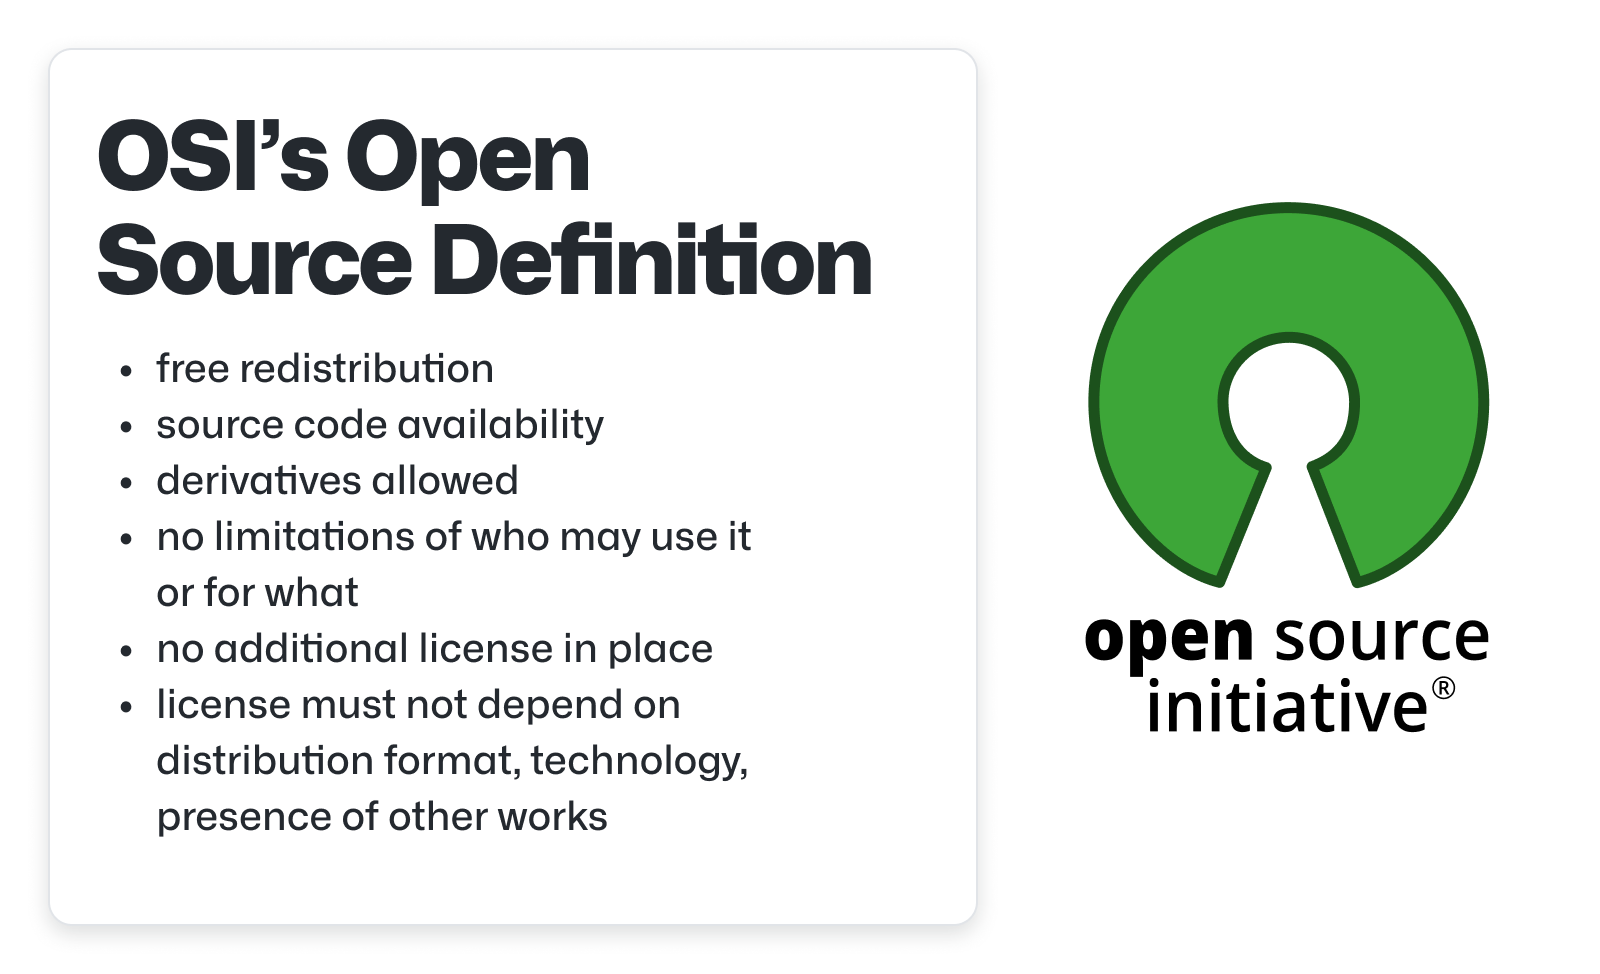
\includegraphics[width=12cm]{figs/osiopensourcedef.png}
\centering
\caption{OSI's Open Source Definition \cite{HaeussgeDevGuide}}
\label{fig:osidef}
\end{figure}



Some of the most popular and influential open-source projects:
\begin{itemize}
    \item Linux: An extremely popular and versatile operating system kernel. Linux powers a vast range of devices from servers and supercomputers to smartphones and embedded systems. It is known for its stability, security, and customization options \cite{fink2003business}. 
    \item Git: A distributed version control system that has become the de facto standard for software development. Git allows developers to track changes to code, collaborate easily, and experiment with different branches of development \cite{loeliger2012version}.  
    \item Apache HTTP Server: One of the most widely used web server software in the world. It is responsible for serving a significant portion of websites on the internet. Apache is known for its reliability, flexibility, and extensive features \cite{fielding1997apache}. 
    \item Python: A high-level, general-purpose programming language that emphasizes readability and ease of use. Python is extremely popular in fields like data science, web development, machine learning, and system administration \cite{srinath2017python}. 
    \item TensorFlow: A free, open-source toolset designed to make machine learning accessible. It offers a wide range of tools, libraries, and a supportive community, so both researchers and developers can create and use powerful ML applications \cite{developers2022tensorflow}.  
\end{itemize}

\subsection{Ownership and Licensing}

The concept of ownership within the open-source software landscape deviates from the traditional models of individual or corporate proprietorship. While thousands of developers might contribute to a single open-source project, the idea of ownership is more accurately framed in terms of rights, intellectual property, and copyright \cite{Codeownership}.  In this context, it's vital to understand the pivotal role of open-source licenses.

In the world of software, open-source licenses reign supreme. The MIT License offers broad permissions for use, modification, and distribution, making it incredibly developer-friendly \cite{saltzer2020origin}. Similarly, the Apache License 2.0 is permissive and emphasizes providing clear copyright and patent notices \cite{sinclair2010license}. For those seeking "copyleft" protection, ensuring that derived works stay open-source, the GNU \ac{gpl} is a common choice \cite{license1989gnu}. 

Licenses establish the boundaries and freedoms granted to users and contributors in utilizing and modifying open-source software \cite{laurent2004understanding}. These licenses come in a variety of forms, each with its own set of rules and restrictions. Some licenses, for example, expressly prohibit the sale of the original software or its derivative versions \cite{madison2003reconstructing}. This is done to safeguard the open-source ethos and prevent commercial exploitation that may stifle community-driven development.

In sum, understanding the intricate interplay of ownership and licensing is essential for navigating the open-source ecosystem. While traditional notions of ownership take a backseat, the principles of intellectual property, copyright, and the specific terms of open-source licenses dictate the rights and responsibilities of all those who interact with this collaborative software model.


\subsection{Morden adoption and future}
\ac{oss} has become a firmly established pillar of the software development landscape, and its influence is poised to grow further in the coming years.  As the open-source community continues to mature and address its challenges, we can anticipate the emergence of even more innovative and powerful solutions driven by this collaborative model.

While the origins of open source can be traced back to the 1960s, with companies like IBM providing free software with their early mainframe systems \cite{moreno2006open}, its widespread adoption has accelerated significantly in recent decades.  Despite the dominance of tech giants like Google, Apple, and Microsoft in the commercial sphere \cite{jacobides2020regulating}, these companies also play a pivotal role in the open-source ecosystem, particularly through contributions on platforms like GitHub.

The substantial impact of open source is exemplified by EU-based companies, which invested an estimated €1 billion in OSS in 2018. This investment yielded a significant return for the European economy, with an estimated contribution ranging from €65 to €95 billion \cite{blind2021impact}.

Figure \ref{fig:bigtechcontributes} underscores the active participation of tech leaders in the open-source movement.  In 2020 alone, 5,709 Google employees submitted over ten commits to GitHub's public code repository.  This was closely followed by contributions from Microsoft, Red Hat, IBM, and others...


\begin{figure}[ht]
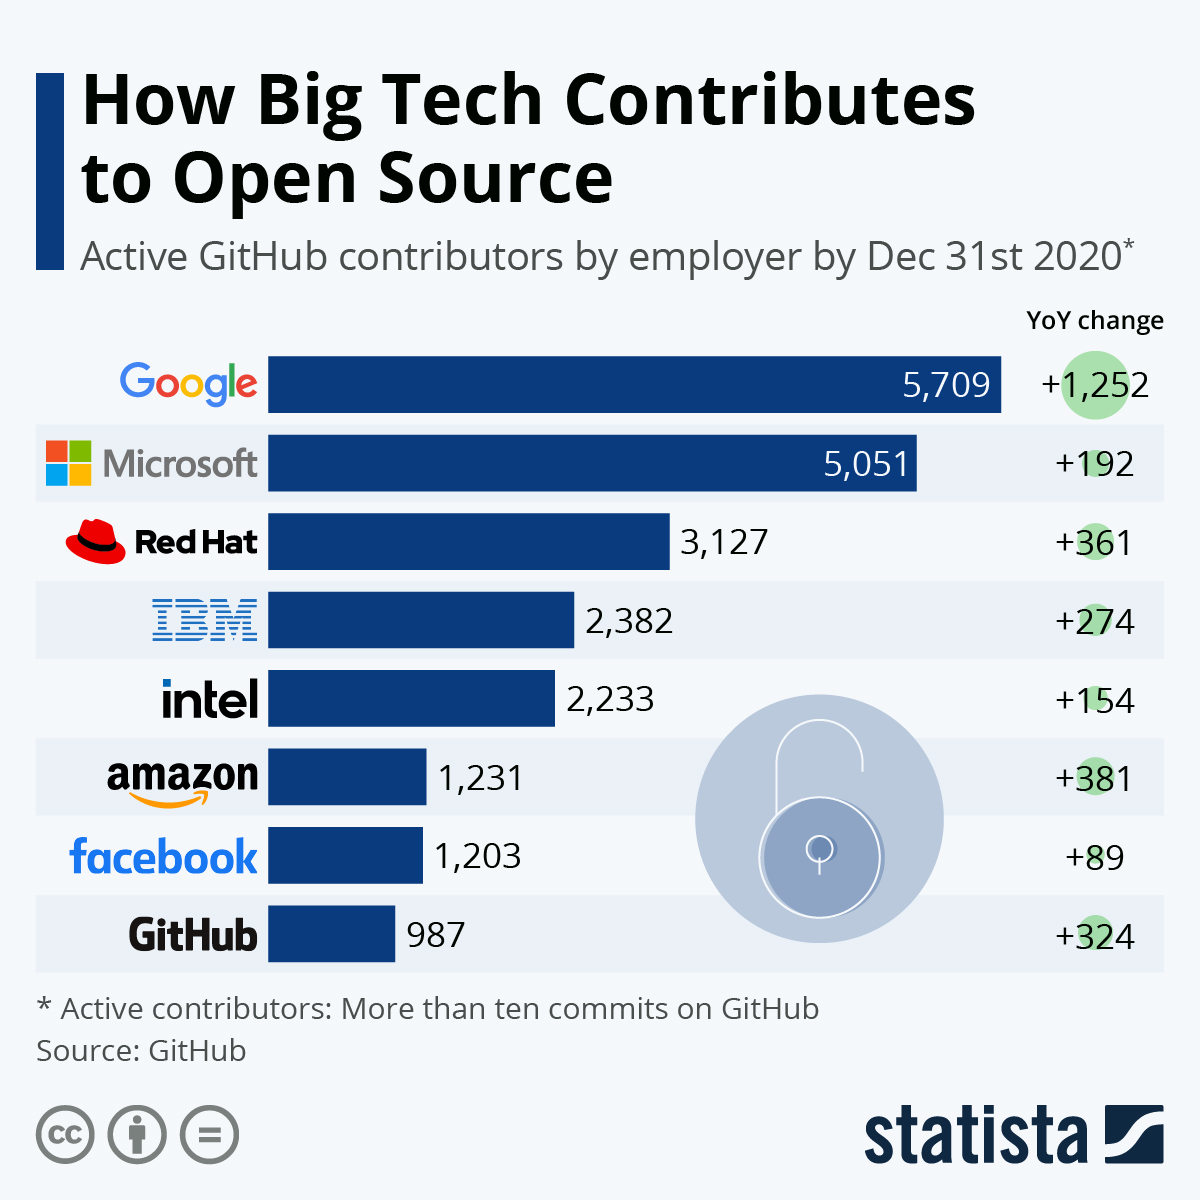
\includegraphics[width=12cm]{figs/bigtechcontributes.jpeg}
\centering
\caption{How How Big Tech Contributes to Open Source \cite{statista2021bigtechopensource}}
\label{fig:bigtechcontributes}
\end{figure}



\clearpage  % This command will start the next section from the new page
               % Add chapter 4
%% This section adds chapter 3
\section{Research methods}

This thesis delves into the complex motivations behind developer participation in open-source projects by combining a \ac{slr} and an in-depth case study. The literature review establishes a robust foundation of knowledge, while the case study illuminates the nuanced social interactions and experiential factors shaping individual developers' decisions to contribute.

\subsection{Systematic Literature Review} \label{slr}

\ac{slr} offers a disciplined research method that promotes a clear, targeted investigation through a well-defined question. This study employs the \ac{slr} methodology as outlined by \citet{Kitchenham}, ensuring a reliable and unbiased review.

\subsubsection{Systematic Literature Review definition}

\ac{slr} is a meticulously planned research approach aiming to identify, evaluate, and synthesize all available evidence related to a clearly defined research question \citep{Kitchenham}. It employs a transparent, reproducible protocol to minimize bias, emphasizing comprehensiveness and critical appraisal of included studies.

The methodology consists of three main phases. First, in the planning phase, researchers must clearly define the research questions that guide the entire review. A detailed review protocol should then be developed, outlining the search strategy (databases, search terms), study selection criteria (e.g., publication types and dates), quality assessment methods, data extraction plans, and the strategy for synthesizing the findings.

The second phase involves conducting the review. This includes identifying research using the search strategy, selecting studies based on the eligibility criteria, critically evaluating study quality, extracting the relevant data, and finally, synthesizing that data using techniques like meta-analysis or thematic analysis.

Finally, the reporting phase focuses on transparently documenting the entire SLR process for reproducibility and critical assessment. Researchers must present the results in a clear manner, addressing the initial research questions and their implications, while also acknowledging any limitations within the review process.

\subsubsection{Systematic Literature Review approach}

Open source software development presents a unique model of collaboration where developers voluntarily contribute their time and expertise. Unlike traditional software engineering environments, motivations in open source extend beyond direct financial compensation. Researchers have investigated these motivations from various perspectives, including psychological, economic, and social factors. This complex landscape can lead to potentially varied interpretations of what drives participation.

The SLR will lay the groundwork for my thesis by providing a thorough understanding of current research on open source developer motivations. Based on the SLR findings, I will be able to identify under-investigated areas or potential gaps in the theoretical frameworks used to explain developer behavior.


\clearpage  % This command will start the next section from the new page


               % Add chapter 3
\section{Systematic Literature Review}

Guided by Kitchenham's SLR framework, this study carefully addressed review planning (defining research questions, developing a protocol), conducting (literature search, study selection, data extraction and quality assessment), and reporting \cite{Kitchenham}.

\begin{figure}[ht]
    \centering
    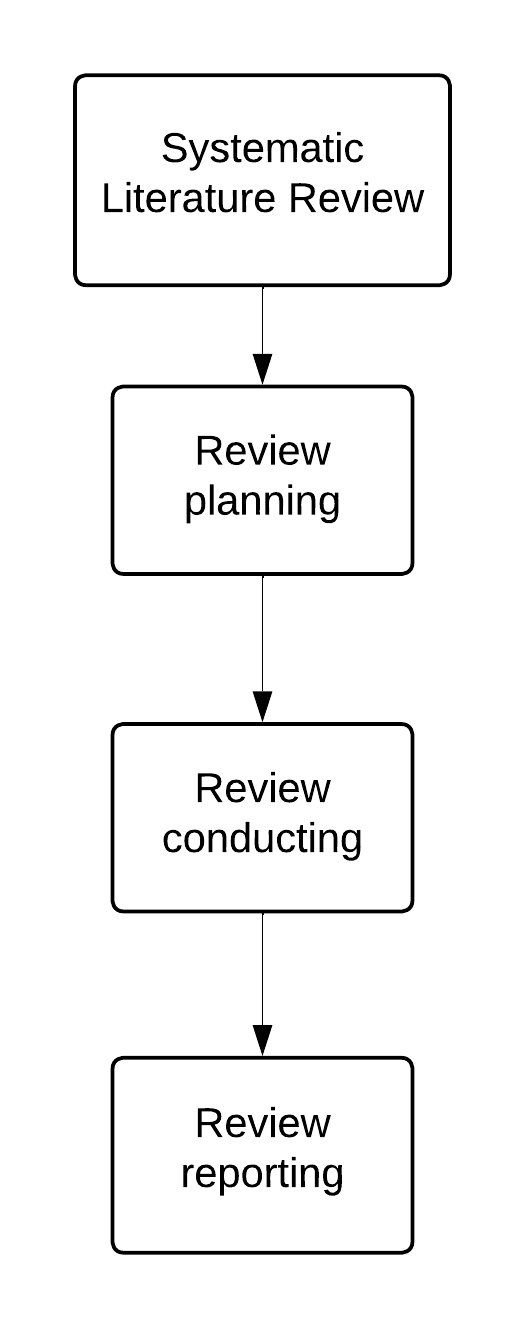
\includegraphics[width=0.3\linewidth]{figs/slr-overview.png}
    \caption{Systematic Literature Review process \cite{Kitchenham}}
    \label{fig:slr-overview}
\end{figure}

The figure \ref{fig:slr-overview} shows an overview of my work to execute a systematic literature review. I meticulously outlined a protocol and defined my overarching research questions 1 and 2. A comprehensive search strategy was then established to pinpoint pertinent articles within electronic databases relevant to the field of open source software motivation. Stringent inclusion and exclusion criteria ensured the selection of methodically sound studies. Following the search, I carefully screened titles and abstracts of retrieved database articles. Studies initially deemed relevant underwent a thorough full-text analysis. This systematic review will culminate in a detailed report encompassing search strategies, selection criteria, the number of articles evaluated at each stage, and an overarching synthesis of the findings.



\subsection{Review planning}

In chapter \ref{researchQuestions}, I explored the process of defining a research question. Here, I will concentrate on developing a protocol for the initial review planning phase of a \ac{slr}. While numerous scientific databases exist online, selecting the most suitable ones for evidence synthesis can be challenging \cite{academicSearchSystems}. This section will offer guidance on database selection and explain the rationale behind different choices.


% Web of Science and Scopus hold a strong reputation as the most reliable and comprehensive citation databases within the academic community \cite{zhu2020tale}. However, 

\subsubsection{Search criteria}
Building on a previous study from Chua and Zhang \cite{Chua_Zhang_2020}, I established inclusion criteria to ensure the selected articles addressed my research questions and utilized strong methodologies:

\begin{itemize}
    \item Research articles and conference papers, peer-reviewed and available through major academic search platforms like Google Scholar, Springer, \ac{ieee}, \ac{acm}, Science Direct.
    \item Restriction to English-language sources.
    \item Disciplines in Computer Science, Software Engineering
    \item Publication date: from 2000 to 2024.
    \item Specific search terms ("open source" OR "open source software") AND ("motivation" OR "contribution challenges" OR "social dynamics impact" OR "interest" OR "contribution barriers") within titles or descriptions.
    \item Prioritization of publications from leading information systems conferences and journals. Ex: ACM/IEEE International Conference on Software Engineering, IEEE Transactions on Software Engineering, Journal of Systems and Software,...
\end{itemize}

These search terms were employed to address the three research questions which are categorized in the table \ref{tab:categoriesSearchTerms}.

\begin{table}[ht]
    \centering
    \begin{tabular}{ | c | l | }
        \hline
        Category & Search terms                                   \\ \hline
        1        & OSS motivation and all synonyms                \\ \hline
        2        & Social dynamics impact on OSS and all synonyms \\  \hline
        3        & Contribution barriers of OSS and all synonyms  \\  \hline
    \end{tabular}
    \caption{Specific categories of search terms}
    \label{tab:categoriesSearchTerms}
\end{table}



\subsubsection{Data source}

To identify relevant literature, I executed our search strings across multiple databases. Each database was queried with the complete set of search strings, yielding varying results. In some instances, identical search strings produced an overabundance of results, while in others, they returned no results. Databases with no results were excluded from further analysis. The selected databases and their corresponding result counts are presented in the following table \ref{tab:initialSearch}.


\begin{table}[ht]
    \centering
    \begin{tabular}{ | l | c | c | c |}
        \hline
        Database       & Category 1      & Category 2     & Category 3      \\ \hline
        Google Scholar & 244 000 results & 17 800 results & 175 100 results \\ \hline
        Springer       & 623 results     & 161 results    & 327 results     \\ \hline
        IEEE           & 396 results     & 68 results     & 48 results      \\ \hline
        Science Direct & 4 200 results   & 97 results     & 15 results      \\ \hline
    \end{tabular}
    \caption{Initial search results from scientific databases}
    \label{tab:initialSearch}
\end{table}



\subsubsection{Inclusion and exclusion criteria}

To maintain a focused and methodologically review, I used inclusion and exclusion criteria to pinpoint studies aligned with my research questions. These criteria served as a consistent filter for all potential sources. The specific criteria are outlined below, and they were applied to every study retrieved from our selected databases.

Inclusion:
\begin{itemize}
    \item Accessible: The research paper must be accessible and downloadable either through LUT Academic Library or online database.
    \item Peer-Reviewed: The paper should be published in a reputable, peer-reviewed journal or conference proceedings. This ensures the quality and credibility of the research.
    \item Relevant to research questions: The paper must directly address the specific research questions at hand.
    \item Methodology transparency: The reasearch and data collection  methodologies must be metioned.
\end{itemize}

Exclusion:
\begin{itemize}
    \item Irrelevant content: Exclude papers that deviate significantly from my research questions or lack a clear connection to the area of study.
    \item Older papers (released before 2000) ought to be disregarded.
    \item Papers having fewer than four pages were removed.
    \item Papers cannot be accessed
    \item Papers were not written in English
    \item Papers topic were about open source but in hardware, economy, environment,... but not software
\end{itemize}

\subsubsection{Study selection}
A further procedures were taken for the final paper selection after applying the inclusion/exclusion criteria to each of the resultant papers.

\begin{itemize}
    \item Review the title, keyword, abstract, description for filtering
    \item Excluding duplicated studies.
    \item Ranking research papers by the number of times they've been cited and relevant to search term by search engine.
\end{itemize}


The initial search across various databases yielded approximately 500,000 potentially relevant papers. Due to resource constraints, the review process was limited to 50 papers per database. Following the application of inclusion and exclusion criteria, along with further selection procedures, a final set of 20 relevant and suitable articles was identified for this SLR. These papers are listed in table \ref{tab:databasePapers}, with full details provided in the Appendix \ref{App:A}. The paper selection process is displayed in the figure \ref{fig:paperselectionprocess}



\begin{figure}[ht]
    \centering
    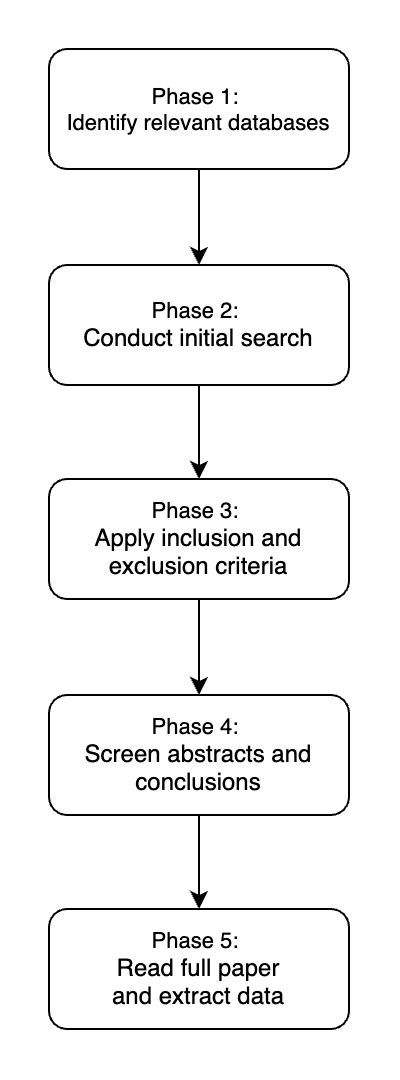
\includegraphics[width=0.3\linewidth]{figs/paperselectionprocess.png}
    \caption{Process of selecting papers for SLR}
    \label{fig:paperselectionprocess}
\end{figure}



\begin{table}[ht]
    \begin{tabular}{| m{7em} | m{5em}| m{18em} | }
        \hline
        Publisher                & Number of articles & Authors                                                                                                                                                                           \\ \hline
        Elsevier                 & 6                  & Bitzer, Schrettl \& Schröder (2007); Choi \& Pruett (2015); Li, Tan \& Teo (2012); Oreg \& Nov (2008); Steinmacher, Silva, Gerosa \& Redmiles (2015); Wu, Gerlach \& Young (2007) \\ \hline
        AISNET                   & 1                  & Ke \& Zhang, P. (2008)                                                                                                                                                            \\ \hline
        IEEE                     & 3                  & Ye \& Kishida (2003); Gerosa, Wiese, Trinkenreich, Link, Robles, Treude \& Sarma (2021); Zhang, Yuxia (2024)                                                                      \\ \hline
        ResearchGate             & 1                  & Zhao, Shengyu (2024)                                                                                                                                                              \\ \hline
        Springer                 & 3                  & Steinmacher, Conte, Gerosa \& Redmiles (2019); Fershtman \& Gandal  (2007); Hannemann \& Klamma (2013) ; Hannemann \& Klamma (2013)                                               \\ \hline
        ACM                      & 3                  & Steinmacher, Conte, Gerosa \& Redmiles (2015); Guizani, Chatterjee, Trinkenreich, May, Noa-Guevara, Russell \& Sarma (2021) ; Hannebauer \& Gruhn (2017)                          \\ \hline
        Informs                  & 1                  & Roberts, Hann \& Slaughter (2006)                                                                                                                                                 \\ \hline
        Taylor \& Francis Online & 1                  & Alexander Hars (2002)                                                                                                                                                             \\ \hline
        EASST                    & 1                  & Freeman (2007)                                                                                                                                                                    \\ \hline
    \end{tabular}
    \caption{Selected papers for SLR}
    \label{tab:databasePapers}
\end{table}


\begin{figure}[ht]
    \hspace*{-0.5in}
    \centering
    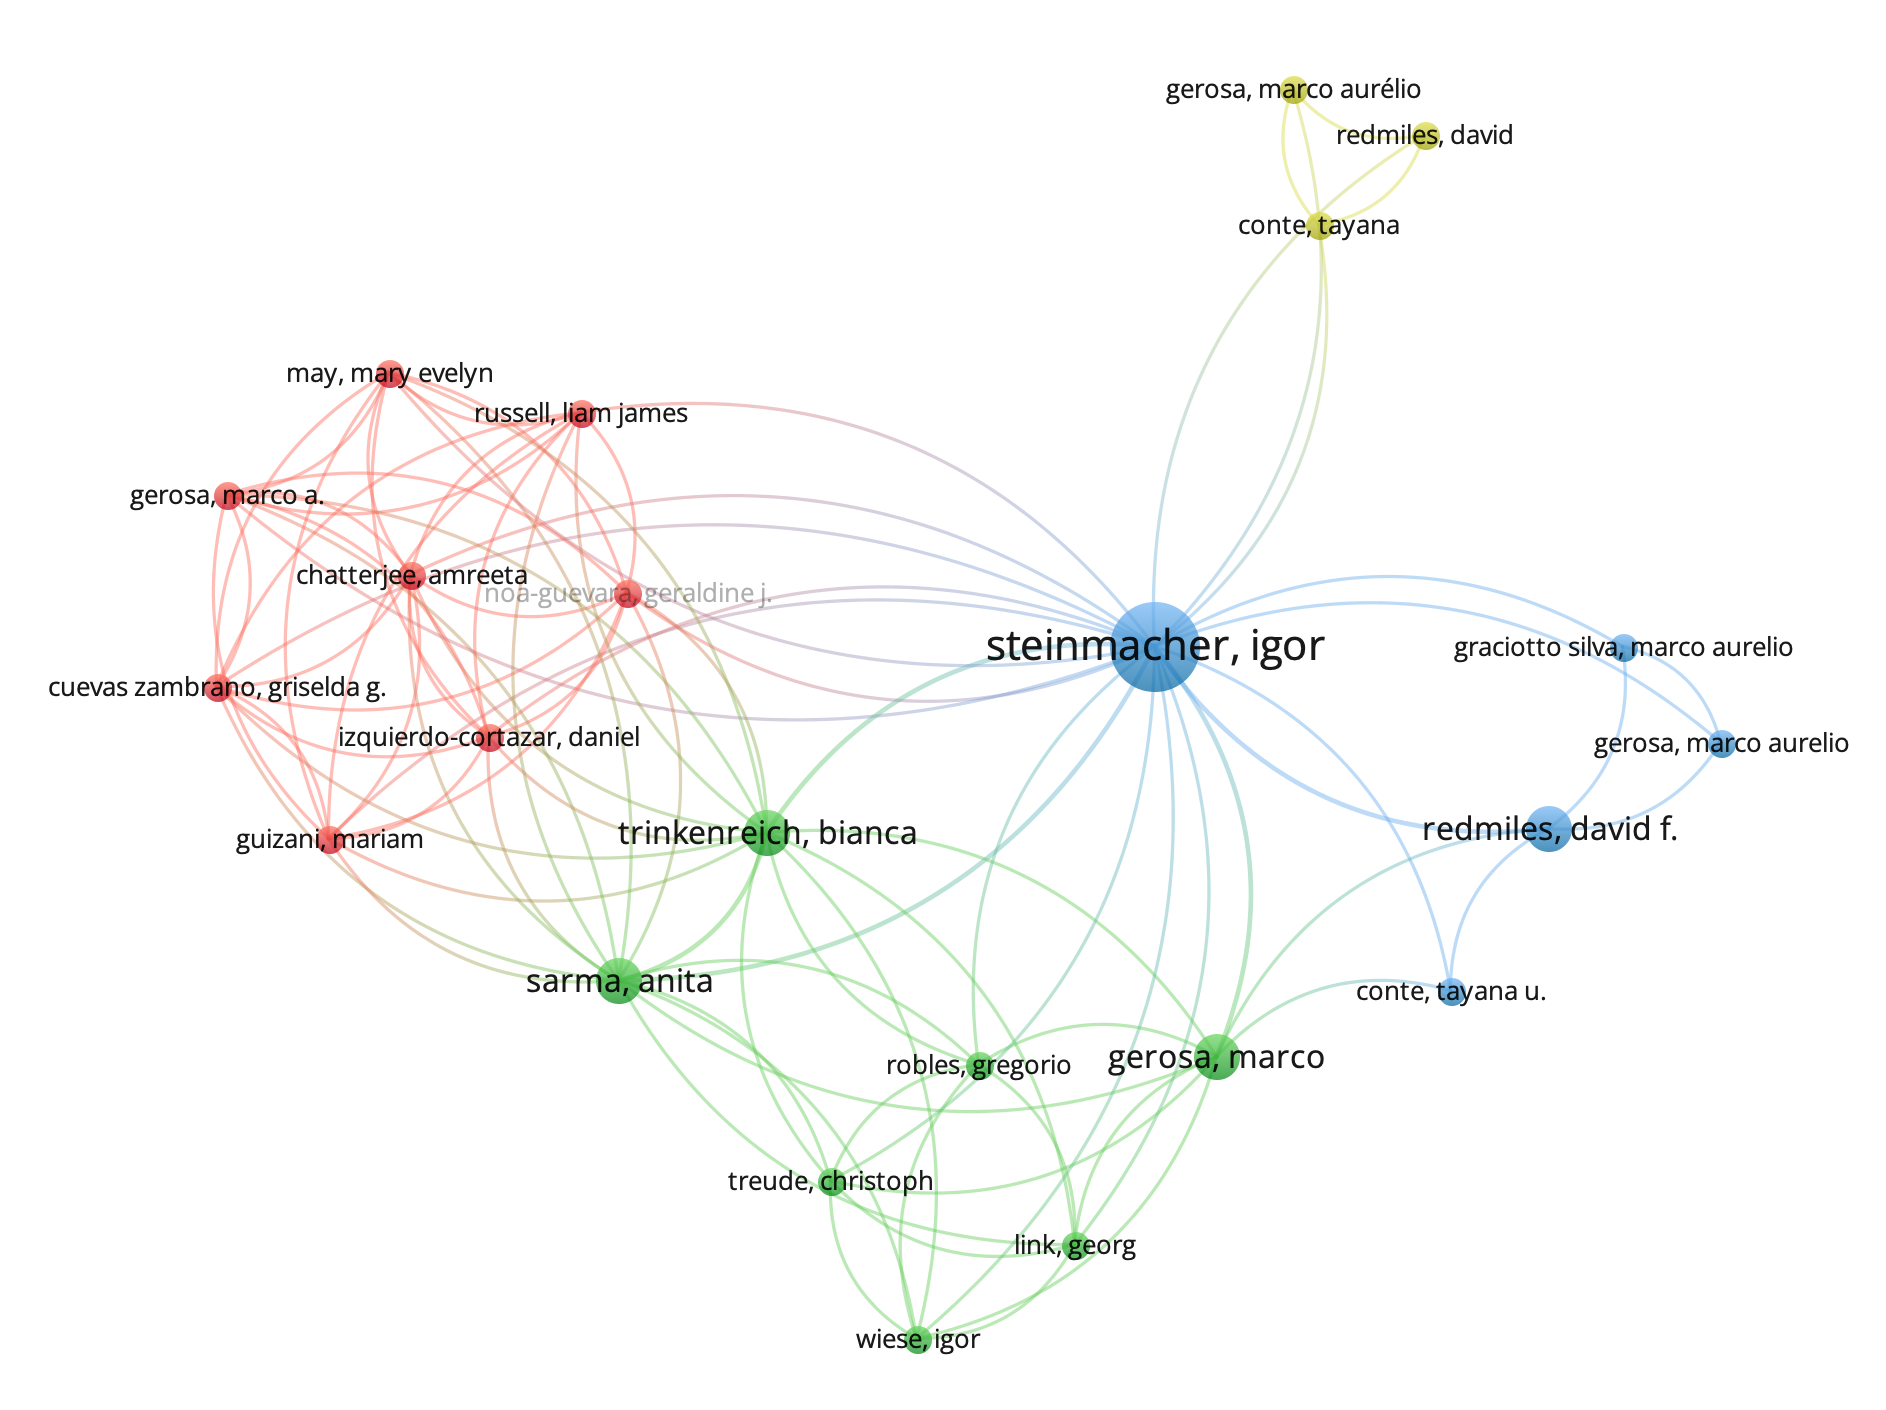
\includegraphics[width=1.1\linewidth]{figs/paperRelation.png}
    \caption{Collaboration relationship between authors of selected papers for SLR}
    \label{fig:paperRelation}
\end{figure}

The figure \ref{fig:paperRelation} depicts the collaboration network between authors of 20 selected papers for a systematic literature review on open-source software motivation, social impact, and challenges. The circles represent authors, and the connecting lines indicate co-authorship on a paper. The size of a circle corresponds to the number of papers an author has co-authored within the dataset. Steinmacher and Igor  appears to be the most prolific author in this dataset, having co-authored papers with several other researchers.

\subsection{Review conducting}

\subsubsection{Extract the data}
An essential stage in an SLR is data extraction. It entails the meticulous collection of precise and pertinent data from the research articles that I have selected for the review. Finding important data points that support the research questions is the first step in this procedure, which also involves methodically arranging the data to make analysis and synthesis of the results easier.
The information that will be taken from each paper is as follows:
\begin{itemize}
    \item Title
    \item Abstract
    \item Authors
    \item Publication date
    \item Database
    \item Keyword
    \item Research method
    \item Data collection method
    \item Answers to research questions
    \item Conclusion
\end{itemize}

\subsubsection{Synthesis}

To systematically analyze the extracted data, we formed two distinct groups (see Table \ref{tab:rq_articleId}) based on their focus:

\begin{itemize}
    \item Group 1: addressing interrelated research questions: This group delves into both research questions 1 and 2. Interestingly, a significant portion of papers addressing question 1 also provide answers to question 2. This overlap suggests a potential relationship between these two research questions. Group 1 comprises a total of 12 carefully selected papers.
    \item Group 2: exclusive focus on research question 3: This group offers a concentrated exploration of research question 3, without addressing the other research areas. Group 2 contains a total of 5 papers, ensuring a targeted examination of this specific question.
\end{itemize}


\begin{table}[ht]
    \centering
    \begin{tabular}{ | c | l |}
        \hline
        Research question & Article ID                                                   \\ \hline
        1                 & A05, A06 , A08 , A09, A10, A11, A12, A13, A15, A16, A17, A18 \\  \hline
        2                 & A05, A06, A07, A09, A10, A12, A13, A16, A17, A18, A19, A20   \\ \hline
        3                 & A01, A02, A03, A04, A14                                      \\ \hline
    \end{tabular}
    \caption{Data synthesis}
    \label{tab:rq_articleId}
\end{table}







\clearpage  % This command will start the next section from the new page
               % Add chapter 5
\section{Review reporting}

The selection process resulted in 20 papers, which were categorized using Wieringa's classification scheme \citep{wieringa2006requirements}. The following categories were relevant to this study:


\begin{itemize}
    \item Evaluation Research: Practical implementation and assessment of techniques or solutions, with a focus on investigating the outcomes.
    \item Validation Research: Examination of novel techniques in a controlled environment, typically a laboratory setting, before practical implementation.
    \item Solution Proposal: Presentation of a solution to a problem, highlighting its advantages, with a higher level of abstraction than validation research.
    \item Philosophical Paper: Introduction of a new perspective on existing concepts by structuring the field through a taxonomy or framework.
    \item Experience Paper: Narration of the author's personal experience, detailing what happened and how it occurred in practice.
    \item Opinion Paper: Expression of the author's personal viewpoint on a specific issue, without relying on related work or research methodologies.
\end{itemize}

The types of contributions were categorized as follows:
\begin{itemize}
    \item Model: Introduction of a new model or framework to address a specific problem.
    \item Method: Presentation of a new method or technique to solve a problem.
    \item Metric: Introduction of a new metric or evaluation criterion to assess the performance of a system or solution.
    \item Process: Description of a new process or workflow to improve efficiency or productivity.
    \item Tool: Introduction of a new tool or software application to facilitate a specific task or process.
\end{itemize}

Here is a systematic map of the selected papers, categorized by research type, contribution type and research question:

The table \ref{tab:systematicMap} presents a breakdown of research on various aspects of open-source software motivation, categorized by research methodology. The primary areas of interest are the factors motivating developers, the influence of social dynamics, and the obstacles to contribution. A significant majority of the studies (16 out of 20) employed evaluation research methods, primarily contributing models and methods to analyze these topics. While a few studies proposed solutions (3) or aimed to validate existing research (1), the emphasis on evaluation research indicates a strong focus on understanding and assessing the current landscape of open-source contributions.

\begin{table}[ht]
    \centering
    \begin{tabular}{| m{7em} | m{5.5em}| m{5.5em} | m{5.5em} | m{3em} |}
        \hline
                                 & Evaluation Research                                                  & Solution Proposal & Validation Research & Total \\
        \hline
        Motivation of developers & Model: P05, P09, P10, P13, P15, P16, P17, P18. Method: P08, P11, P12 & Process: P06      &                     & 12    \\ \hline
        Social dynamics impact   & Model: P20. Metric: P07                                              &                   & Metric: P19         & 3     \\ \hline
        Contribution barriers    & Model: P01, P04, P14                                                 & Model: P02, P03   &                     & 5     \\ \hline
        Total                    & 16                                                                   & 3                 & 1                   & 20    \\ \hline
    \end{tabular}
    \caption{Systematic map of selected papers}
    \label{tab:systematicMap}
\end{table}


\subsection{RQ1: Primary motivation for developers contributing in open source}

The primary aim of this research is to uncover the reasons why developers participate in OSS projects. Each study chosen for this analysis was examined for any empirically identified or assessed motivations, such as career advancement, skill development, altruism, or enjoyment. By understanding these motivations, I hope to gain insights into what drives individuals to contribute to OSS projects and how this knowledge can be used to foster greater participation and collaboration in the future.

A visual depiction of the quantity of published articles on the different incentives that encourage developers to contribute to open source software projects can be seen in the chart \ref{fig:articleMotivationCount}. The amount of articles devoted to each motivation is shown on the x-axis, while the motivations are grouped along the y-axis.

The data reveals a diverse range of motivations, with social factors emerging as prominent drivers of participation. The most extensively researched motivations, Signaling/Recognition (11 articles) and Play Value (10 articles), highlight the importance of social recognition and the inherent enjoyment developers derive from contributing to OSS projects. Personal Interest, Altruism and Ideology, and Learning also receive significant attention in the literature, with 8 articles dedicated to each. These motivations underscore the multifaceted nature of developer engagement, encompassing personal passions, a desire to contribute to the greater good, and the pursuit of knowledge and skill development.

Conversely, the least explored motivations are Role Transformation and Improving Software Quality, with only 2 articles each. This disparity suggests that while the existing literature acknowledges the potential impact of these motivations, they remain relatively understudied compared to social factors.

The diversity of motivations highlighted in the chart underscores the complexity of the open-source community. It is evident that developers are driven by a combination of social, personal, ideological, and career-oriented factors. This nuanced understanding is crucial for organizations and communities seeking to attract and retain developers. Tailored strategies that address the diverse motivations of developers are essential for fostering a thriving and sustainable open-source ecosystem.

Moreover, the chart reveals the need for further research into less-explored motivations, such as Role Transformation and Improving Software Quality. A deeper understanding of these motivations could provide valuable insights into how to incentivize contributions that directly enhance the quality and impact of OSS projects.

\begin{figure}[ht]
    \centering
    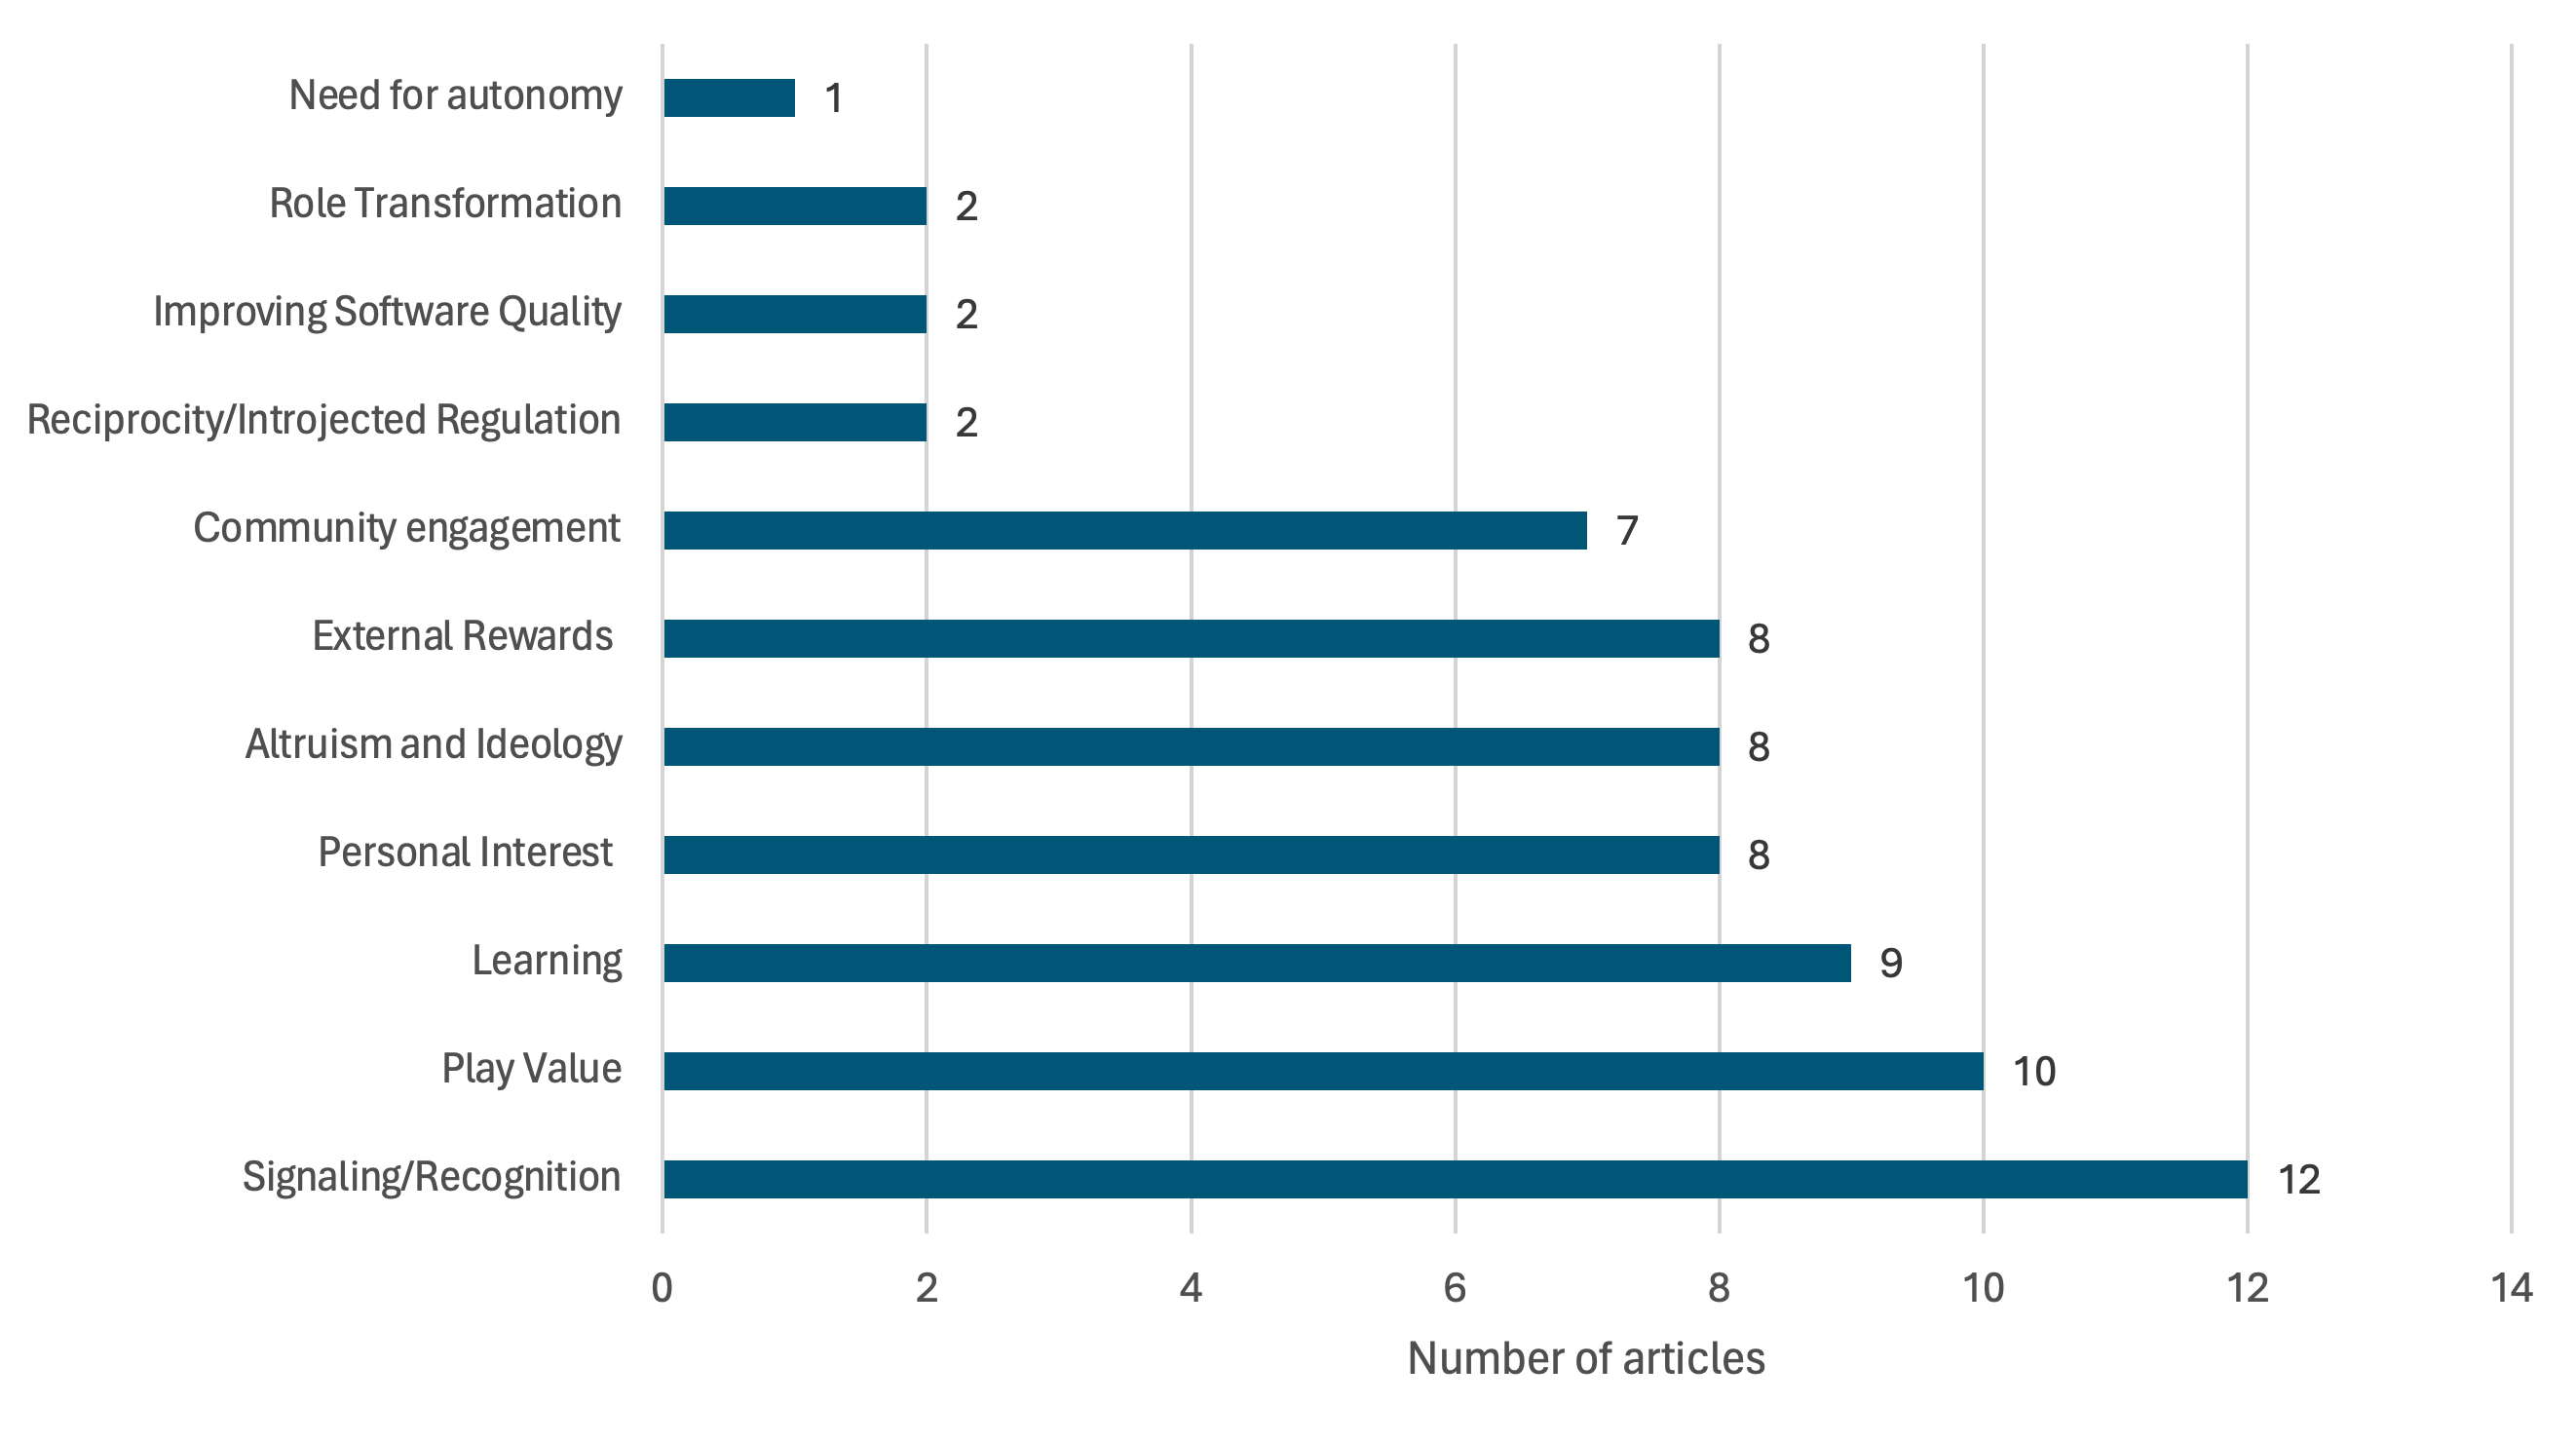
\includegraphics[width=1\linewidth]{figs/articleMotivationCount.png}
    \caption{Number of articles mentioning each motivation}
    \label{fig:articleMotivationCount}
\end{figure}

\subsubsection{Intrinsic motivations}
My exploration of developer motivation in open-source software projects begins with intrinsic motivations, the internal drivers that fuel participation for personal satisfaction rather than external rewards. This encompasses a broad spectrum of factors, including: play value, the inherent enjoyment derived from the coding process; community engagement, the sense of belonging and collaboration found within OSS projects; learning, the opportunity to develop new skills and expand technical knowledge; personal interest, the desire to work on projects that align with individual passions; altruism and ideology, the belief in contributing to a greater good and supporting the open-source philosophy; need for autonomy, the freedom to work independently and creatively; and reciprocity/introjected regulation, the desire to contribute back to the community and maintain a sense of personal responsibility for the project's success. I will delve deeper into each of these intrinsic motivations in the following sections, examining their unique influence on developer behavior within the OSS landscape.

1. Play value

In contrast to traditional software development, which often prioritizes external rewards like monetary compensation and career advancement, OSS projects offer a unique space where play value emerges as a central driving force. Play value, in this context, encapsulates the inherent enjoyment, intellectual stimulation, and creative fulfillment developers experience through the act of programming and problem-solving \parencite{05bitzer2007intrinsic, 06ye2003toward, 08zhang2024paid, 09lakhani2005hackers, 11gerosa2021shifting, 12choi2015characteristics,13li2012leadership,16ke2008motivations,17alexander2002working, 18oreg2008exploring}. Let's examine why this is such a powerful motivator.

For many developers, OSS represents a playground for experimentation and innovation. Unburdened by strict commercial deadlines or rigid specifications, they are free to explore novel ideas, test unconventional approaches, and engage in the iterative process of building software purely for the intrinsic satisfaction it provides .  The act of turning concepts into functional code can be deeply rewarding.

OSS communities often tackle complex technical problems that demand creative solutions.  Developers who are drawn to intrinsically motivating challenges revel in the opportunity to dissect intricate issues, devise elegant workarounds, and optimize code performance. This continuous learning process creates a sense of mastery and accomplishment that fuels further engagement.

Commercial software development typically necessitates compromises – feature trade-offs, adherence to proprietary standards, and prioritization of market demands over pure technical curiosity. In contrast, OSS projects offer developers a liberating space to exercise their technical creativity without external pressures. This autonomy nourishes problem-solving and innovation for its own sake.

The collaborative aspect of OSS can itself be a form of play.  Engaging with fellow developers, brainstorming solutions, exchanging knowledge, and contributing to a shared creation can be intellectually stimulating and enjoyable. This connection fosters a playful sense of experimentation and discovery within the community.


2. Community engagement

The act of conceptualizing the open-source community as a metaphorical family, united in pursuit of shared objectives, can be a powerful catalyst for developer participation \parencite{05bitzer2007intrinsic,07zhao2024openrank, 08zhang2024paid, 09lakhani2005hackers, 13li2012leadership, 16ke2008motivations, 17alexander2002working}. This collaborative environment fosters contributions aimed at communal advancement, even when they may not yield immediate personal gain for the individual developer. Participation in open-source projects can be fueled by a profound sense of belonging and an alignment of personal values with those of project teams and the open-source movement at large.

The chart \ref{fig:motivationDimension} underscores the complex interplay of motivations that drive developer participation in open-source projects. While social factors are paramount, career considerations and political beliefs also play a significant role. This diversity of motivations highlights the need for a nuanced understanding of the open-source community and tailored strategies to attract and retain developers.

\begin{figure}[ht]
    \centering
    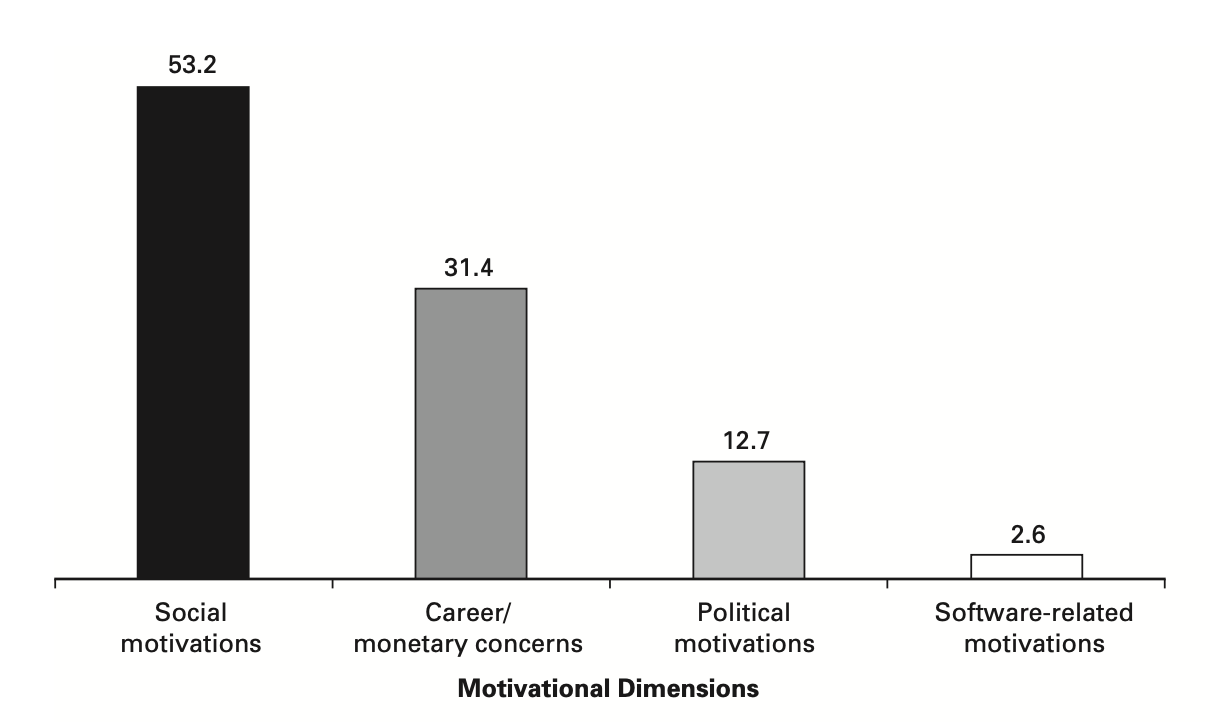
\includegraphics[width=0.7\linewidth]{figs/motivationDimension.png}
    \caption{As a proportion of all contributors to OSS, developers by motivation class \citep{ghosh2002free}}
    \label{fig:motivationDimension}
\end{figure}

Additionally,  a conviction regarding the inherent value of open-source code, paired with a perceived responsibility to contribute to the free and OSS ecosystem, serves as a significant motivator for developers. Cultivating a sense of belonging and fostering a shared purpose within the community or project team can thus be instrumental in empowering individuals to become active participants and contributors in the open-source software development landscape.



3. Learning

Research consistently identifies learning as a primary impetus for individuals to actively engage in OSS communities \parencite{06ye2003toward, 07zhao2024openrank, 08zhang2024paid, 09lakhani2005hackers, 10wu2007empirical, 11gerosa2021shifting, 12choi2015characteristics, 17alexander2002working, 18oreg2008exploring}. OSS projects present multifaceted learning environments; developers are drawn to the inherent opportunities to acquire knowledge from the systems themselves, to collaborate and gain insights from fellow community members, and to reciprocally disseminate their own expertise.

Participation within OSS communities extends beyond the purely technical exchange of knowledge, encompassing a rich social dimension. By directly engaging in open-source projects, developers immerse themselves in a collaborative network of peers, often spanning skill levels and expertise. This fosters a dynamic learning ecosystem where individuals benefit from informal mentorship opportunities, observing problem-solving approaches employed by more experienced contributors, and receiving constructive feedback that accelerates their professional growth.

Moreover, the act of contributing to a shared knowledge base empowers developers and reinforces self-efficacy. The potential for continuous self-development, the pursuit of mastery, and the ability to give back to a community dedicated to knowledge-sharing serve as profound and enduring sources of motivation for many software contributors.

4. Personal interest

Some developers get involved in open-source projects due to a personal interest in the subject matter or a desire to address a specific need or problem. This intrinsic motivation is driven by a passion for the technology, a curiosity about the project's objectives, or a personal connection to the software's utility. Developers who are personally invested in the project's success are more likely to contribute actively and engage with the community \citep{06ye2003toward,07zhao2024openrank,09lakhani2005hackers,11gerosa2021shifting,12choi2015characteristics,13li2012leadership,16ke2008motivations,17alexander2002working}

The concept of the "personal itch," as articulated by Eric S. Raymond, illuminates a key motivator for developer participation in OSS projects \citep{holtgrewe2004articulating}. Individuals often engage in OSS development to address a specific problem or augment functionality that directly aligns with their personal or professional needs. The desire to create a solution that may not otherwise exist, driven by this personal necessity, serves as a potent catalyst for engagement.

Furthermore, the inherent intellectual challenge of solving complex programming problems stands as a significant motivator for developers seeking to contribute to open-source initiatives. The opportunity to grapple with intricate coding puzzles, apply problem-solving strategies, and ultimately contribute to the solution can be deeply fulfilling for those driven by a passion for programming.

The sense of creativity fostered within the OSS landscape is another powerful draw. Developers are empowered to express their ingenuity, explore innovative solutions, and continuously hone their skills through the development of tools or solutions that serve their own requirements or those related to their work. This blend of personal utility, creative expression, and continuous learning establishes a compelling environment that attracts and sustains developer involvement.

5. Altruism and ideology

OSS development thrives in part due to the contributions of individuals motivated by altruism and ideological convictions \citep{07zhao2024openrank,08zhang2024paid,10wu2007empirical,11gerosa2021shifting,13li2012leadership,16ke2008motivations,17alexander2002working,18oreg2008exploring}. This section explores these factors and their influence on developer participation. A significant driver for many developers is the inherent satisfaction derived from assisting others. Contributing to open-source projects allows them to directly improve software used by a wider community. This collaborative environment fosters a sense of purpose, as developers witness the positive impact of their work on others

Many developers are drawn to  the core principles of open-source software, including transparency, collaboration, and the democratization of technology. Participation allows them to contribute to a development model that emphasizes open access and fosters a sense of community.  Additionally, developers can be motivated by a desire to create software that benefits the greater good by being freely available and readily modifiable. This aligns with their altruistic desire to contribute to society and maintain strong social bonds.

Altruism and ideological alignment with open-source principles play a vital role in propelling developer participation. Both the satisfaction of helping others and the commitment to open-source ideals create a compelling environment that attracts and retains developers within the OSS ecosystem.

6. Autonomy

The OSS environment provides a platform where developers can exercise a high degree of autonomy, making it particularly attractive to those valuing self-determination. The ability to select projects of interest, dictate their involvement, and contribute independently fulfills the intrinsic need for autonomy. This freedom to innovate and pursue solutions without rigid constraints becomes a compelling motivator, drawing developers who seek a sense of control and ownership over their contributions \citep{16ke2008motivations}.

Unlike traditional software development environments that might be constrained by rigid hierarchies or top-down management styles, the open-source model empowers developers to chart their own path. They can choose to focus on areas that align with their passions, explore new technologies, or experiment with novel approaches without the need for constant external approval.  This sense of agency and self-direction is deeply fulfilling for those who thrive in environments where their initiative and creativity are valued.

7. Reciprocity and introjected regulation

Open-source communities thrive on a powerful sense of reciprocity. Developers who have directly benefited from freely available open-source software often feel a deep-seated obligation to give back, fueling their participation and ensuring the continued growth of the ecosystem. This desire to repay the community for the invaluable resources they've received becomes a motivating force \citep{11gerosa2021shifting,13li2012leadership}.

Additionally, introjected regulation plays a role in influencing developer behavior. The internalization of expectations can lead to feelings of pride, guilt, or shame regarding contributions to open-source projects. This desire to maintain a positive self-image, live up to personal standards, and avoid negative emotions can significantly drive participation as developers strive to meet both their own expectations and those they perceive the community holds.

\subsubsection{Extrinsic motivations}

Beyond the intrinsic factors explored in the previous chapter, extrinsic motivations also play a significant role in driving developer participation in open-source projects. This chapter delves into these external factors, including the potential for signaling skills and experience to potential employers, garnering recognition and building reputation within the open-source community, and potentially obtaining external rewards such as monetary compensation or job opportunities.

I will also examine how extrinsic motivators can intersect with a developer's  desire to improve software quality. Contributions to high-profile projects can serve as a powerful signal of competence, while active participation may lead to opportunities to collaborate with skilled developers and gain valuable experience.  Furthermore, I will explore the concept of role transformation: how continued involvement in the open-source landscape can elevate a developer's standing, potentially opening doors to leadership roles, consulting positions, or  job offers within companies heavily invested in open-source technologies.

1. Signaling and recognition

Participating in OSS projects allows developers to publicly showcase their abilities and commitment \citep{05bitzer2007intrinsic,06ye2003toward,07zhao2024openrank,08zhang2024paid,09lakhani2005hackers,10wu2007empirical,11gerosa2021shifting,12choi2015characteristics,13li2012leadership,15roberts2006understanding,17alexander2002working,18oreg2008exploring}. Within the highly competitive software development field, OSS contributions provide concrete evidence of a developer's abilities, enhancing their reputation and potentially unlocking new opportunities.  Open-source involvement demonstrates not only technical skills but also a dedication to the broader community and a drive for innovation.


Open-source projects offer developers a platform to display their talents to potential employers, boosting their professional standing. Unlike traditional resumes or interviews that provide a more limited view, OSS contributions offer real-world proof of a developer's capabilities. Employers often see active participation as indicative of both technical skill and the ability to collaborate effectively in a team setting.

The recognition garnered from fellow developers within the open-source community serves as a powerful motivator. The open-source model promotes collaboration, transparency, and continuous improvement, resulting in a space where contributions are acknowledged and celebrated. This validation from peers acts as a potent incentive for developers to further advance their skills and continue making meaningful contributions to projects they're passionate about.

Participating actively in open-source projects helps developers establish solid professional reputations and establish themselves as authorities in their area. Respect is earned by developers in the community via regular, excellent contributions, perceptive analysis, and positive engagement. Their professional status is enhanced by this acknowledgment, which also opens up new opportunities for networking, cooperation, and career advancement. In the end, using their open-source work as a portfolio serves the interests of the developer as a whole as well as the individual developer.

2. Improving software quality


Many developers participate in open-source projects to create superior software that is available to a larger audience and benefits the community \citep{13li2012leadership,15roberts2006understanding}. Open-source development encourages collaboration among developers with diverse backgrounds who share knowledge and work towards shared objectives. By utilizing the combined intelligence and resources of the community, developers create robust, reliable software that addresses the changing needs of users across various industries and fields. This democratization of software development ensures innovative solutions are freely available for anyone to use, modify, and share.

Through involvement in open-source projects, developers access and contribute to software that caters to their specific needs and preferences, often surpassing proprietary options. Unlike closed-source software, which may have proprietary limitations and licensing costs, open-source projects offer greater flexibility and transparency. Developers can freely examine, adjust, and improve the code as needed, empowering them to create tailored solutions that are more efficient, secure, and adaptable. This collaborative and iterative approach to software development not only promotes innovation but also fosters a sense of ownership and pride among contributors, motivated by the collective impact of their work on the wider community.


3. External rewards

While publicly discussions often prioritize the significance of intrinsic motivations, extrinsic rewards such as promotions, financial incentives, increased compensation, and professional advancement remain potent drivers of developer participation in open-source projects \citep{05bitzer2007intrinsic,06ye2003toward,07zhao2024openrank,11gerosa2021shifting,13li2012leadership,15roberts2006understanding,17alexander2002working,18oreg2008exploring}. Tangible rewards hold substantial appeal, particularly for those who utilize open-source involvement as a strategic tool for career development and financial gain. Within a highly competitive labor market emphasizing demonstrable skills and practical experience, active open-source contributions tangibly augment a developer's professional credentials and enhance their overall marketability.

Developers may be drawn by the potential financial returns derived from open-source participation, such as new job opportunities or consulting contracts. By establishing a visible record of expertise and successful contributions, developers attract the attention of companies or clients who value their skills, potentially leading to lucrative positions. Beyond traditional employment, open-source involvement can serve as a foundation for supplementary income streams, such as consulting services, training workshops, or speaking engagements, which cultivate both financial rewards and professional recognition.

Furthermore, the pursuit of career advancement and professional distinction strongly motivates developers to engage with open-source projects. Establishing oneself as a thought leader or subject matter expert within the community cultivates opportunities for leadership positions, mentorship roles, or invitations to esteemed conferences and industry events.  The visibility and reputation fostered through such contributions heighten a developer's standing and create new pathways for professional growth and development.  Ultimately, while intrinsic motivations undeniably fuel enthusiasm and dedication,  extrinsic rewards remain indispensable in attracting and sustaining long-term participation in open-source initiatives.

A study examining the dynamics of paid and volunteer open-source developers within the Rust project has revealed significant disparities in their contribution behaviors \citep{08zhang2024paid}. Notably, core developers who receive compensation demonstrate a higher frequency of contributions compared to volunteers \ref{fig:contribution_frequency}. This suggests that financial incentives may play a role in driving sustained engagement.

\begin{figure}[ht]
    \centering
    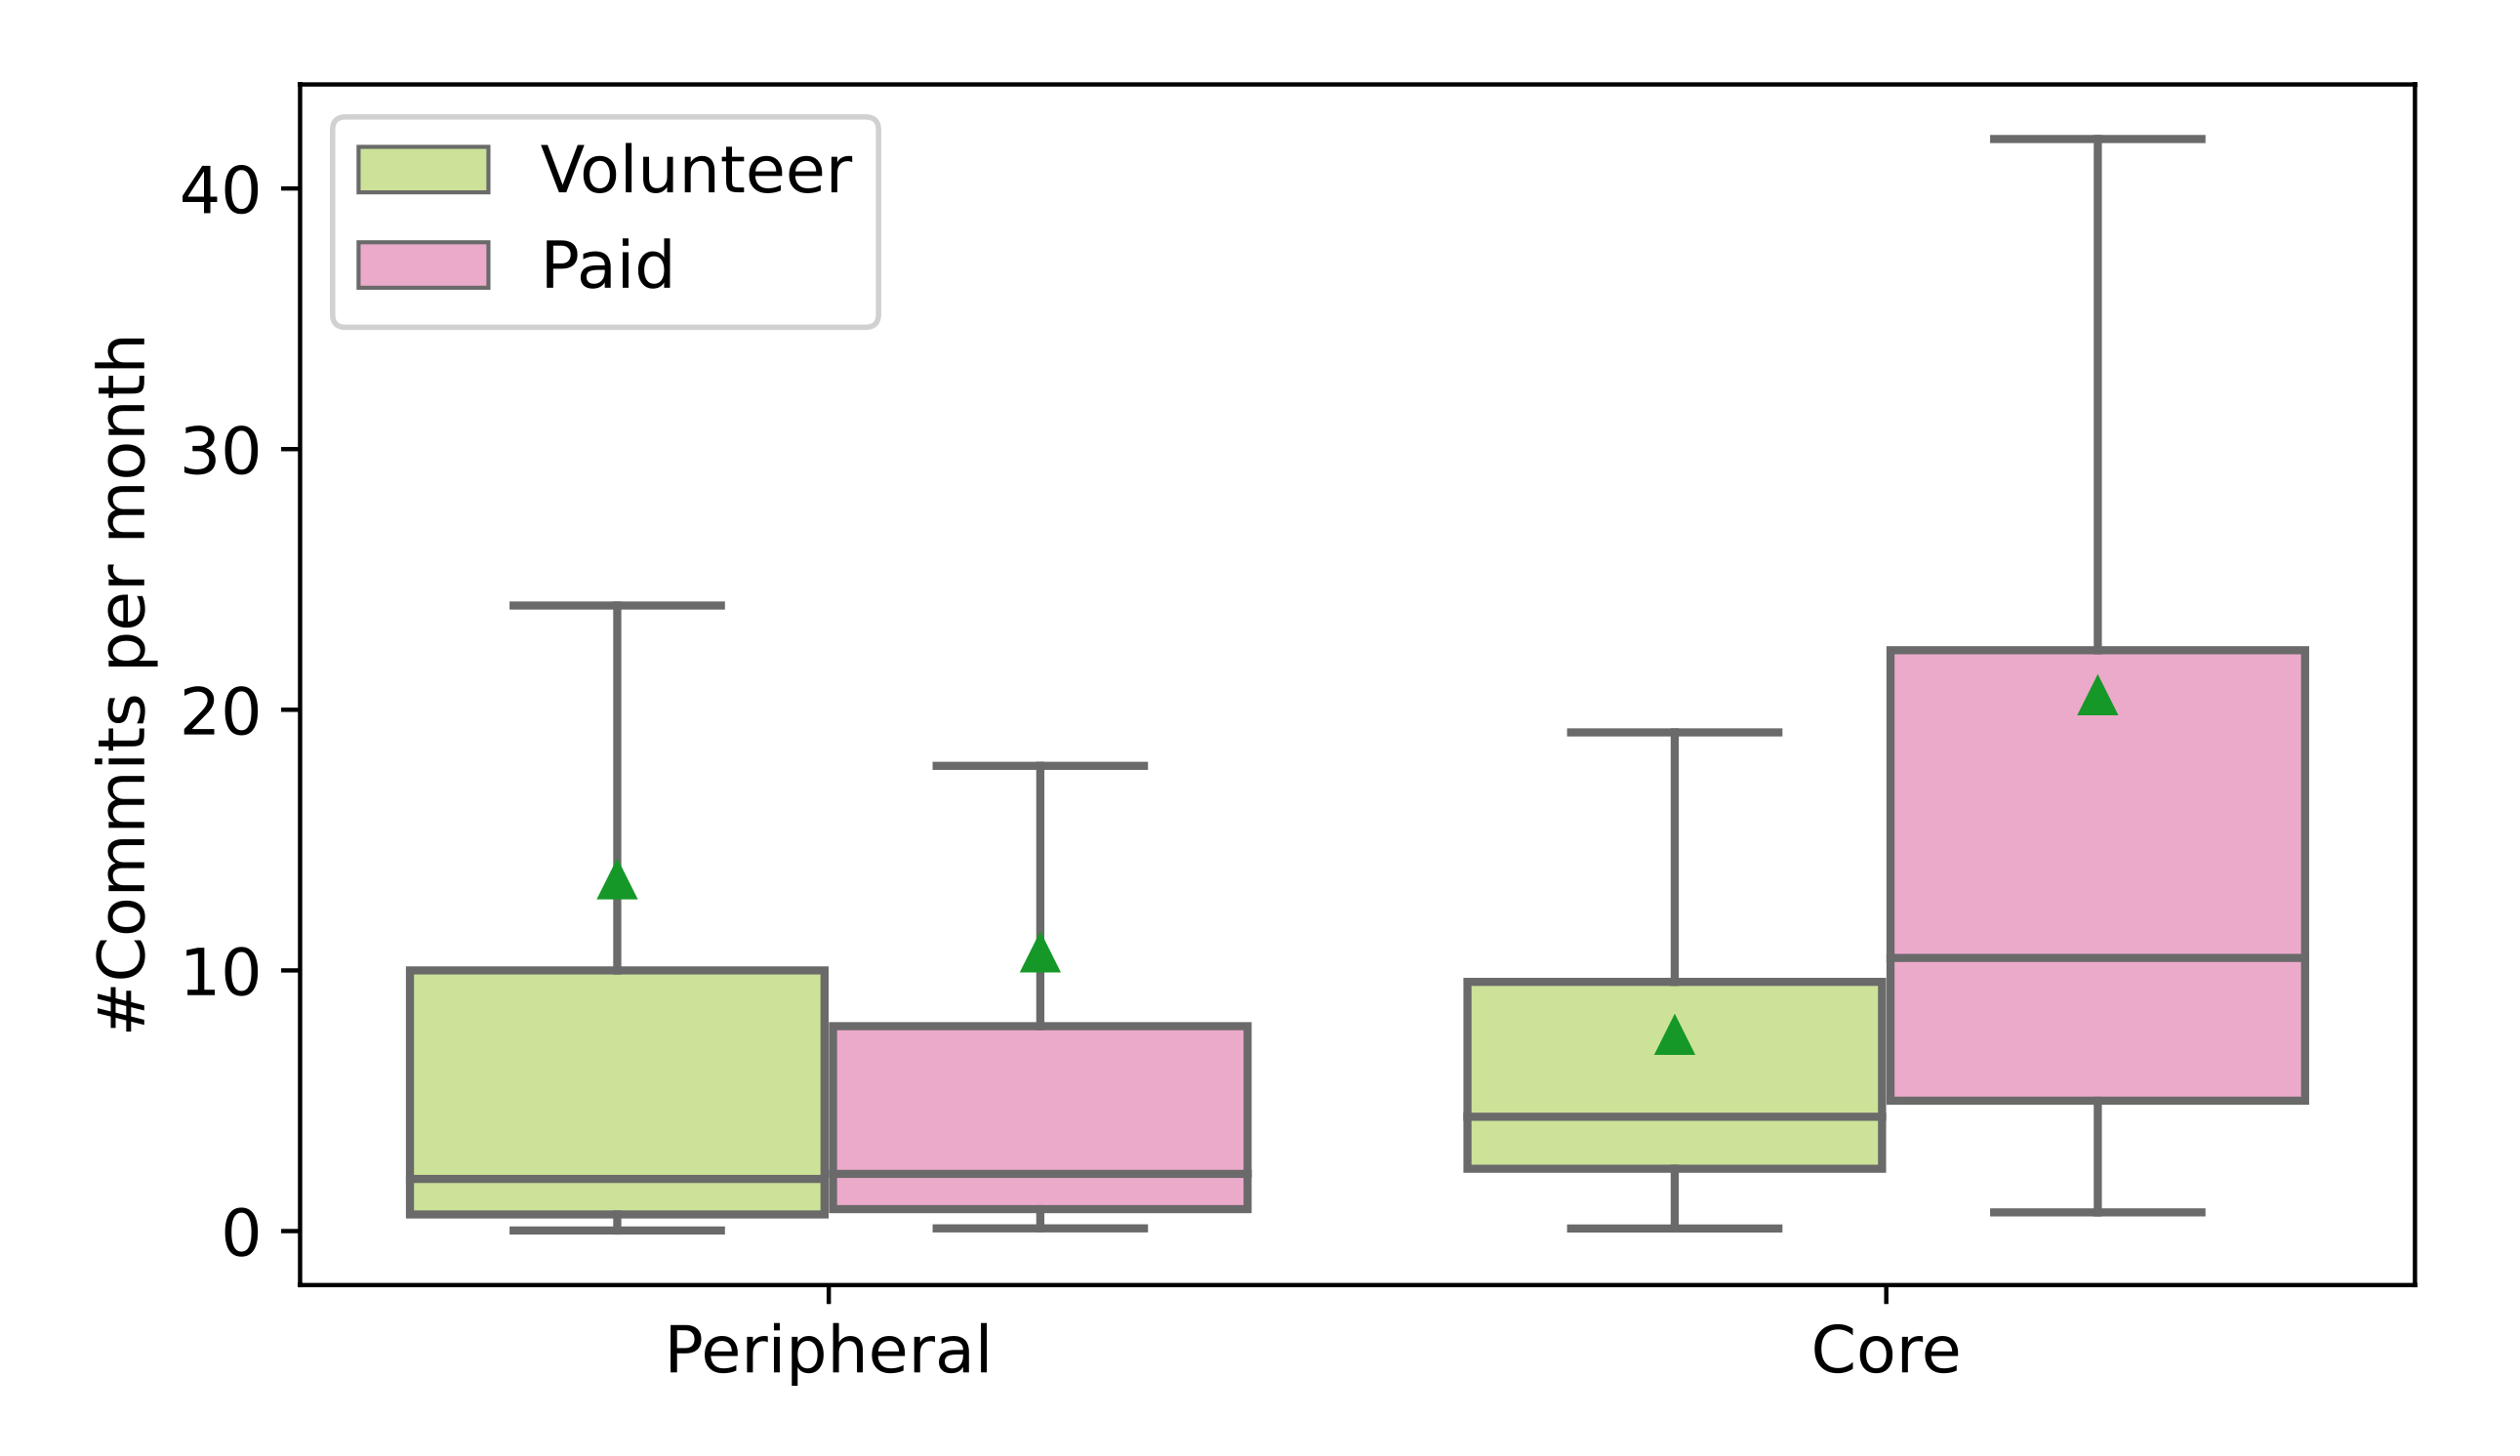
\includegraphics[width=0.65\linewidth]{figs/Contribution_frequency.png}
    \caption{How often paid and volunteer developers contribute to Rust project \citep{08zhang2024paid}}
    \label{fig:contribution_frequency}
\end{figure}


Moreover, commits from one-time paid developers tend to be larger in scope, potentially encompassing more impactful code changes than those of one-time volunteers. This highlights a possible correlation between compensation and the magnitude of contributions. Peripheral paid developers exhibit a higher inclination towards implementing new features compared to unpaid contributors. This trend underscores how financial incentives might influence not only the quantity but also the innovative nature of contributions within the open-source ecosystem.

Collectively, these findings illustrate the complex dynamics of mixed-motivation OSS projects. Understanding these distinctions is crucial for project maintainers seeking to effectively leverage the collaborative potential of both paid and volunteer contributors, ultimately strengthening the sustainability of OSS projects.

4. Role transformation

One of the defining characteristics of OSS projects is the transformation of roles.  Unlike traditional software development models, where users and developers occupy distinct positions, OSS communities blur these lines.  Anyone, from seasoned developers to individuals with technical curiosity, can become a contributor.  This inclusive nature fosters a sense of ownership and empowers users to actively shape the project's evolution.  The potential to transition from user to developer offers a compelling incentive for participation, fostering a community where everyone's voice is valued, and diverse perspectives are encouraged \citep{06ye2003toward,09lakhani2005hackers}.

The progression of OSS systems and communities throughout time is depicted in figure \ref{fig:roleMotivation}.  The responsibilities of developers and users become more entwined as projects expand and mature.  Users who use the program for work-related or personal purposes at first may become active contributors in the future out of a desire to improve the project, take care of certain issues, or impart their knowledge to the community.  This shift in position is evidence of the cooperative spirit of open-source development, where users are empowered to influence the software they use and contribute to a common goal of advancement and innovation.


\begin{figure}[ht]
    \centering
    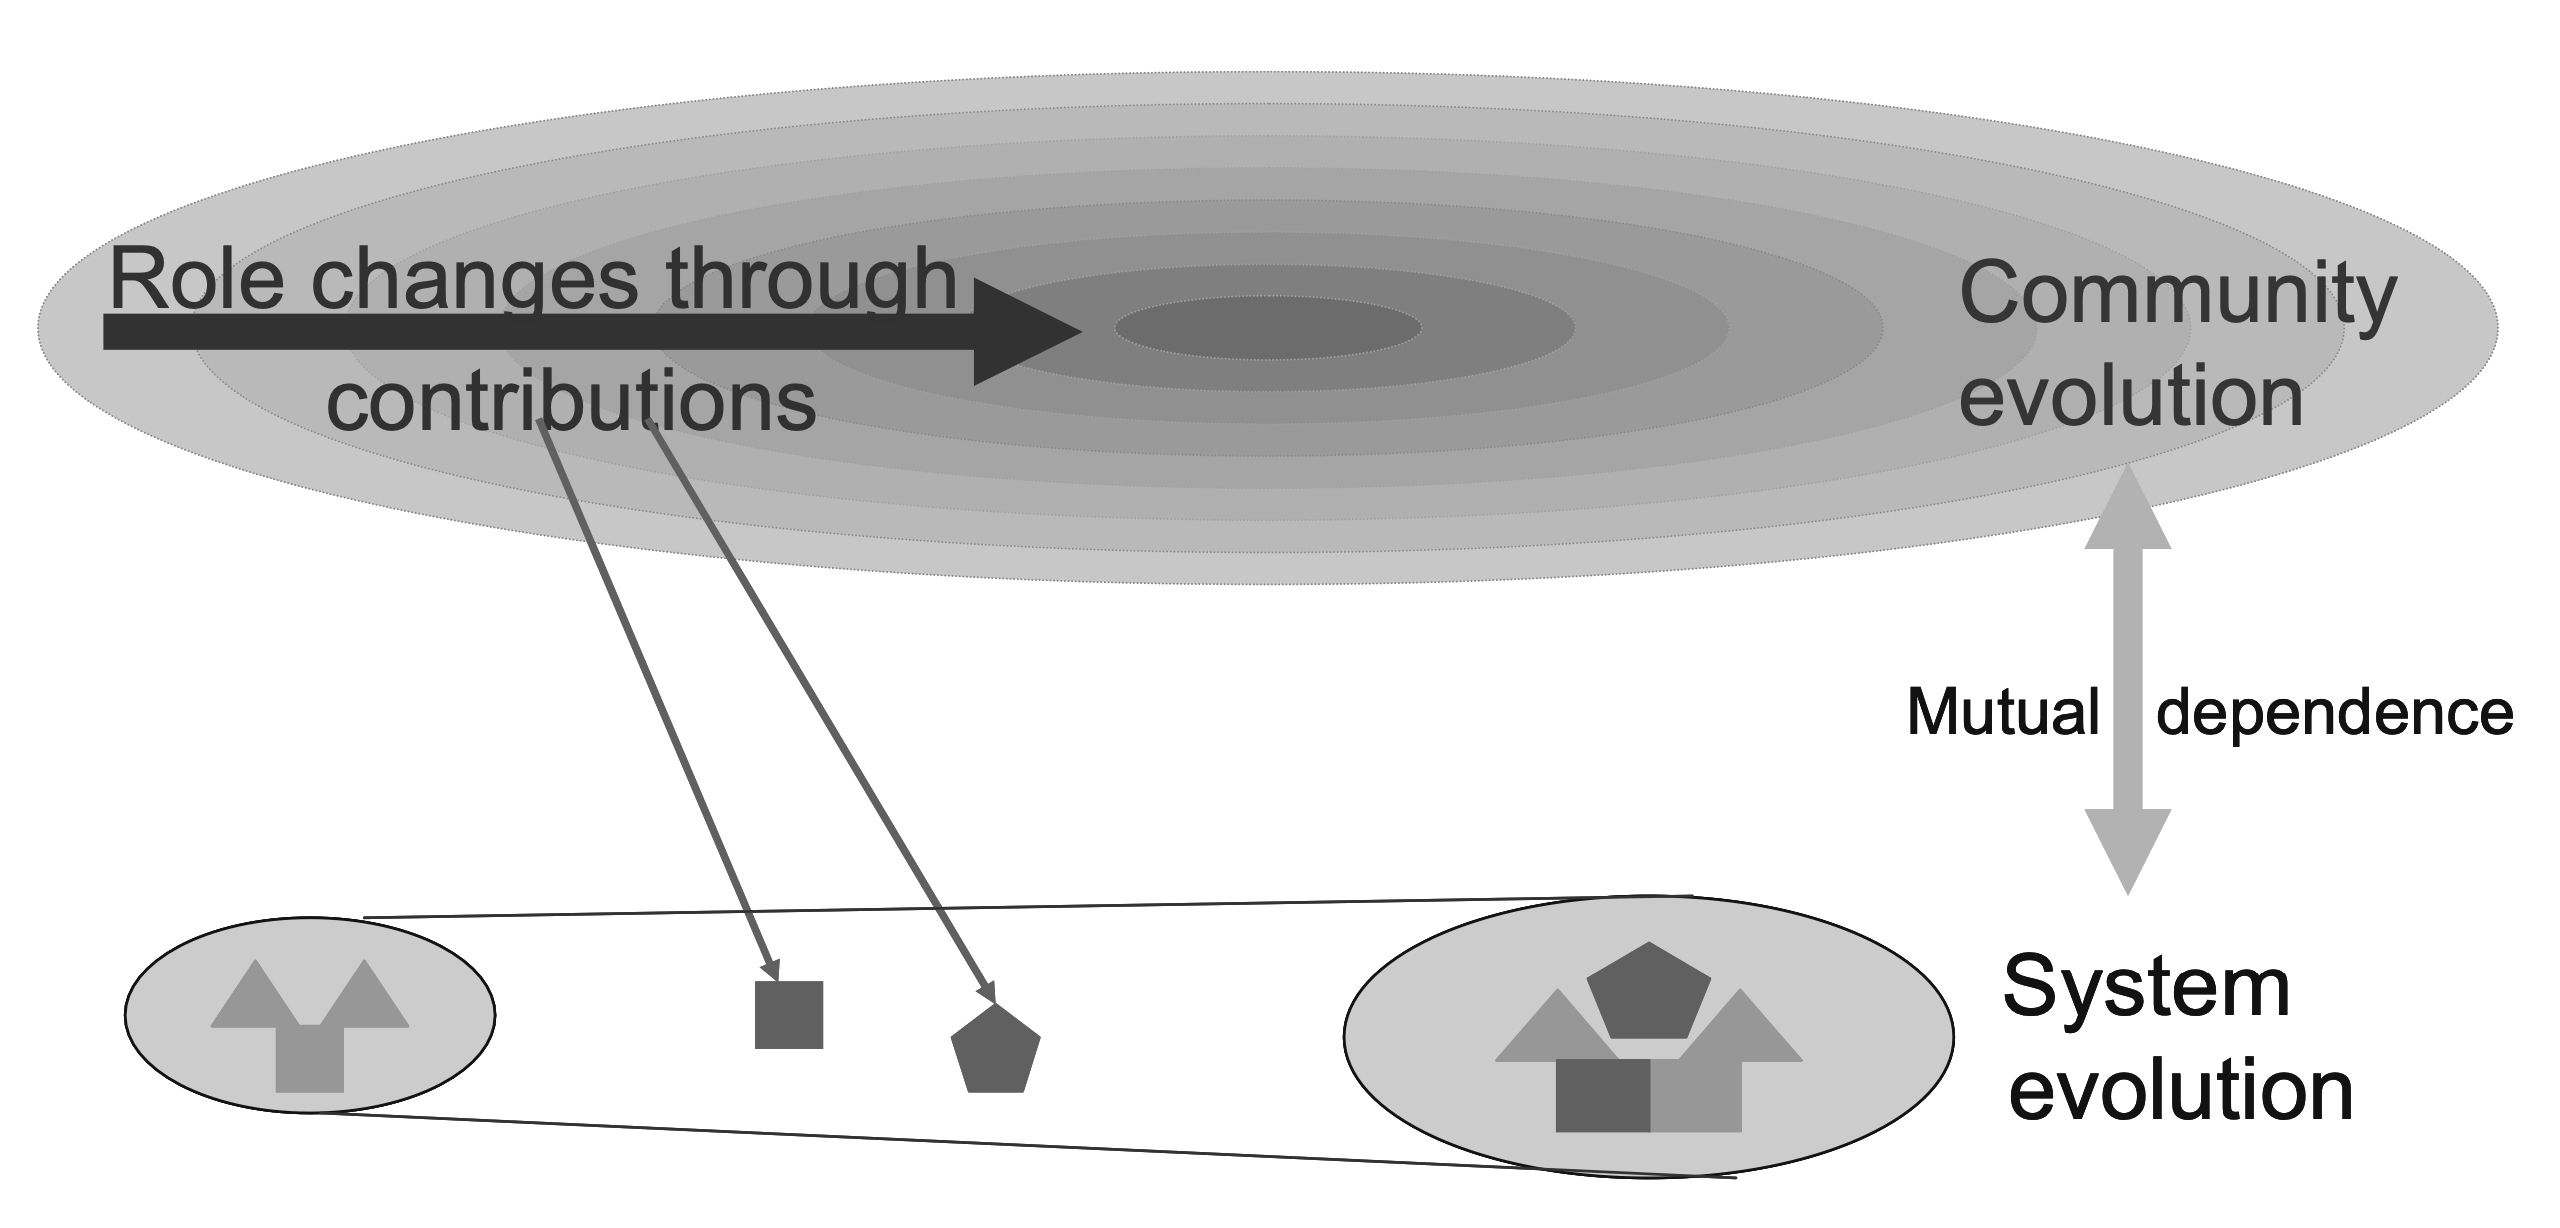
\includegraphics[width=0.65\linewidth]{figs/roleMotivation.png}
    \caption{How open-source software systems and communities grow together \citep{06ye2003toward} }
    \label{fig:roleMotivation}
\end{figure}



Moreover, the opportunity to directly fulfill user needs is a key motivator for developers contributing to open-source projects. Regardless of whether these needs stem from professional or personal pursuits, developers within the OSS community are driven by a desire to create software that tackles real-world challenges and improves user experiences. This direct link between developers and users fosters a collaborative atmosphere where both sides gain from shared knowledge and a commitment to ongoing enhancement.

\subsection{RQ2: Impact of social dynamics}

In addition to investigating the motivations of developers, this research also examined the significant influence of social dynamics on the participation of developers in open-source projects. Through a comprehensive analysis of 13 pertinent studies selected from a pool of over 20 papers, this research has yielded several key findings. These findings highlight the multifaceted nature of developer engagement in open-source initiatives and underscore the importance of social interactions in shaping participation patterns. The subsequent sections will elaborate on these findings, providing a nuanced understanding of the interplay between individual motivations and social forces within the open-source software development ecosystem.

\subsubsection{Community interaction}
The level of interaction within an open-source community is a significant determinant of developer participation. Active communication channels, encompassing forums, mailing lists, and chat platforms, provide essential avenues for collaboration, knowledge sharing, and mutual assistance. These interactions foster a sense of community and belonging, encouraging developers to actively engage with the project and contribute their expertise. Conversely, projects with limited or ineffective communication channels may struggle to attract and retain contributors, as developers may feel isolated or lack the necessary support to make meaningful contributions \citep{05bitzer2007intrinsic,11gerosa2021shifting,20freeman2007material}.


Empirical research consistently demonstrates that developers derive substantial satisfaction from collaborative endeavors and the opportunity to assist others within the open-source ecosystem. Collaboration and teamwork are not merely instrumental means to achieve project goals but are also intrinsically rewarding for developers. The sense of community engendered by open-source projects, along with the opportunity to interact with peers and contribute to a shared endeavor, are integral to the ethos of open-source software development.

The establishment of robust communication infrastructure and feedback mechanisms is paramount for sustaining active developer participation. Clear, transparent, and efficient communication facilitates the resolution of technical issues, the exchange of innovative ideas, and the coordination of efforts among team members \citep{05bitzer2007intrinsic,13li2012leadership}. Moreover, constructive feedback loops enable developers to learn from each other, refine their skills, and enhance the quality of their contributions. Cultivating a supportive and communicative environment fosters a sense of camaraderie and shared purpose, thereby augmenting developer engagement and productivity.

The integration of social features within open-source platforms, such as mechanisms for connecting individuals seeking assistance with those willing to provide it, can substantially enhance community interactions and support. The open-source ethos is intrinsically predicated on collaboration and the open exchange of knowledge, and social platforms facilitate these interactions by creating virtual spaces for developers to connect, communicate, and collaborate. The sense of belonging to a community of like-minded individuals fosters camaraderie, mutual assistance, and a shared sense of purpose, all of which contribute to sustained engagement and project success.

In order to encourage engagement and retention in open-source communities, it is imperative that seasoned developers be present and eager to assist beginners. Mentorship programs enable inexperienced developers to overcome obstacles, learn new skills, and blend in with the community by offering them priceless advice, support, and encouragement. This knowledge transfer across generations is critical to the long-term viability and expansion of open-source initiatives. Open-source communities may draw and keep a wide range of contributors by creating a warm, accepting atmosphere that values knowledge sharing and mentoring. This ensures the ongoing creativity and vitality of the open-source software ecosystem.



\subsubsection{Networking opportunities}
Novice contributors often transition their initial motivations towards career-oriented goals, leveraging open-source projects as a portfolio to showcase their skills to potential employers \citep{05bitzer2007intrinsic,11gerosa2021shifting}. Participation in these projects offers invaluable networking opportunities, fostering connections with industry professionals and paving the way for career advancement \citep{10wu2007empirical,11gerosa2021shifting,13li2012leadership}. By demonstrating their expertise and building a reputation within the open-source community, developers can attract job offers, consulting opportunities, and further professional development. Moreover, the open-source environment allows developers to gain experience with diverse technologies, tools, and methodologies, broadening their skillset and making them more adaptable to the evolving demands of the tech industry.

Open-source projects serve as a platform for developers to connect with industry peers, experts, and potential employers \citep{10wu2007empirical,11gerosa2021shifting,13li2012leadership}. These connections can lead to collaborations on new projects, expanding professional networks and opening doors to career growth opportunities. The collaborative nature of open-source projects allows developers to establish relationships with like-minded individuals, fostering a supportive community that encourages knowledge sharing and mutual growth.  Additionally, engaging with established open-source communities can provide developers with exposure to industry best practices, coding standards, and project management methodologies, further enhancing their professional capabilities.

Open-source projects are inherently collaborative environments, providing developers with ample opportunities to share knowledge, learn from others, and enhance their skills. The exchange of ideas, feedback on code, and exposure to diverse perspectives within the community foster continuous learning and skill improvement. Through interactions with other developers, mentorship, and exposure to new ideas and technologies, developers are motivated to stay engaged and contribute to the project's ongoing success \citep{05bitzer2007intrinsic,06ye2003toward,09lakhani2005hackers,13li2012leadership}. This culture of continuous learning and knowledge sharing also helps developers stay abreast of the latest trends and innovations in the tech industry, ensuring their skills remain relevant and in demand.


\subsubsection{Community culture and support }

Engaged and supportive open-source communities act as a catalyst for developer contributions by offering assistance, constructive feedback, and a sense of belonging. This collaborative atmosphere nurtures knowledge sharing, mutual support, and a strong sense of community among developers. Ultimately, positive social interactions and a supportive environment within these communities drive increased motivation and sustained engagement among developers. \citep{10wu2007empirical,12choi2015characteristics,13li2012leadership,16ke2008motivations}.

Social coding platforms have revolutionized the open-source landscape, shifting the culture from its traditional hacker-centric roots to a more inclusive, collaborative community. By lowering barriers to entry, these platforms have made open-source projects more accessible and welcoming to newcomers, regardless of their technical expertise \citep{06ye2003toward,11gerosa2021shifting}. They foster a sense of belonging and encourage participation through features like issue tracking, discussion forums, and code review tools, promoting knowledge sharing and collaborative problem-solving. This cultural shift has not only broadened the pool of contributors but has also led to more diverse perspectives and innovative solutions within the open-source ecosystem.

Roles within OSS communities are dynamic and fluid, allowing members to assume greater responsibilities by contributing meaningfully to projects. As individuals transition between roles, they actively influence the social dynamics and structure of the community, ultimately driving its evolution \citep{06ye2003toward}. This flexibility enables OSS communities to adapt and thrive in response to the evolving needs of projects and the diverse contributions of their members.


Open-source platforms that promote collaboration and offer diverse avenues for appreciation, ranging from formal accolades to informal gestures like awarding stars to projects, significantly enhance the sense of belonging and recognition among community members. Active engagement in these communities allows developers to gain recognition for their contributions, cultivate a positive reputation, and establish a personal brand within the wider developer community \citep{11gerosa2021shifting,13li2012leadership}.

The paper "OpenRank Leaderboard: Motivating Open Source Collaborations Through Social Network Evaluation in Alibaba" presents a study conducted to explore the impact of the OpenRank Leaderboard on open source collaborations within Alibaba's projects \citep{07zhao2024openrank}. The research methodology involved a mixed-methods approach, including case studies, surveys, analysis of project metrics data, semi-structured interviews, and thematic coding. The study focused on seven open source projects initiated by Alibaba, aiming to investigate how gamified leaderboards can motivate collaboration and drive innovation in software development.

\begin{figure}[ht]
    \centering
    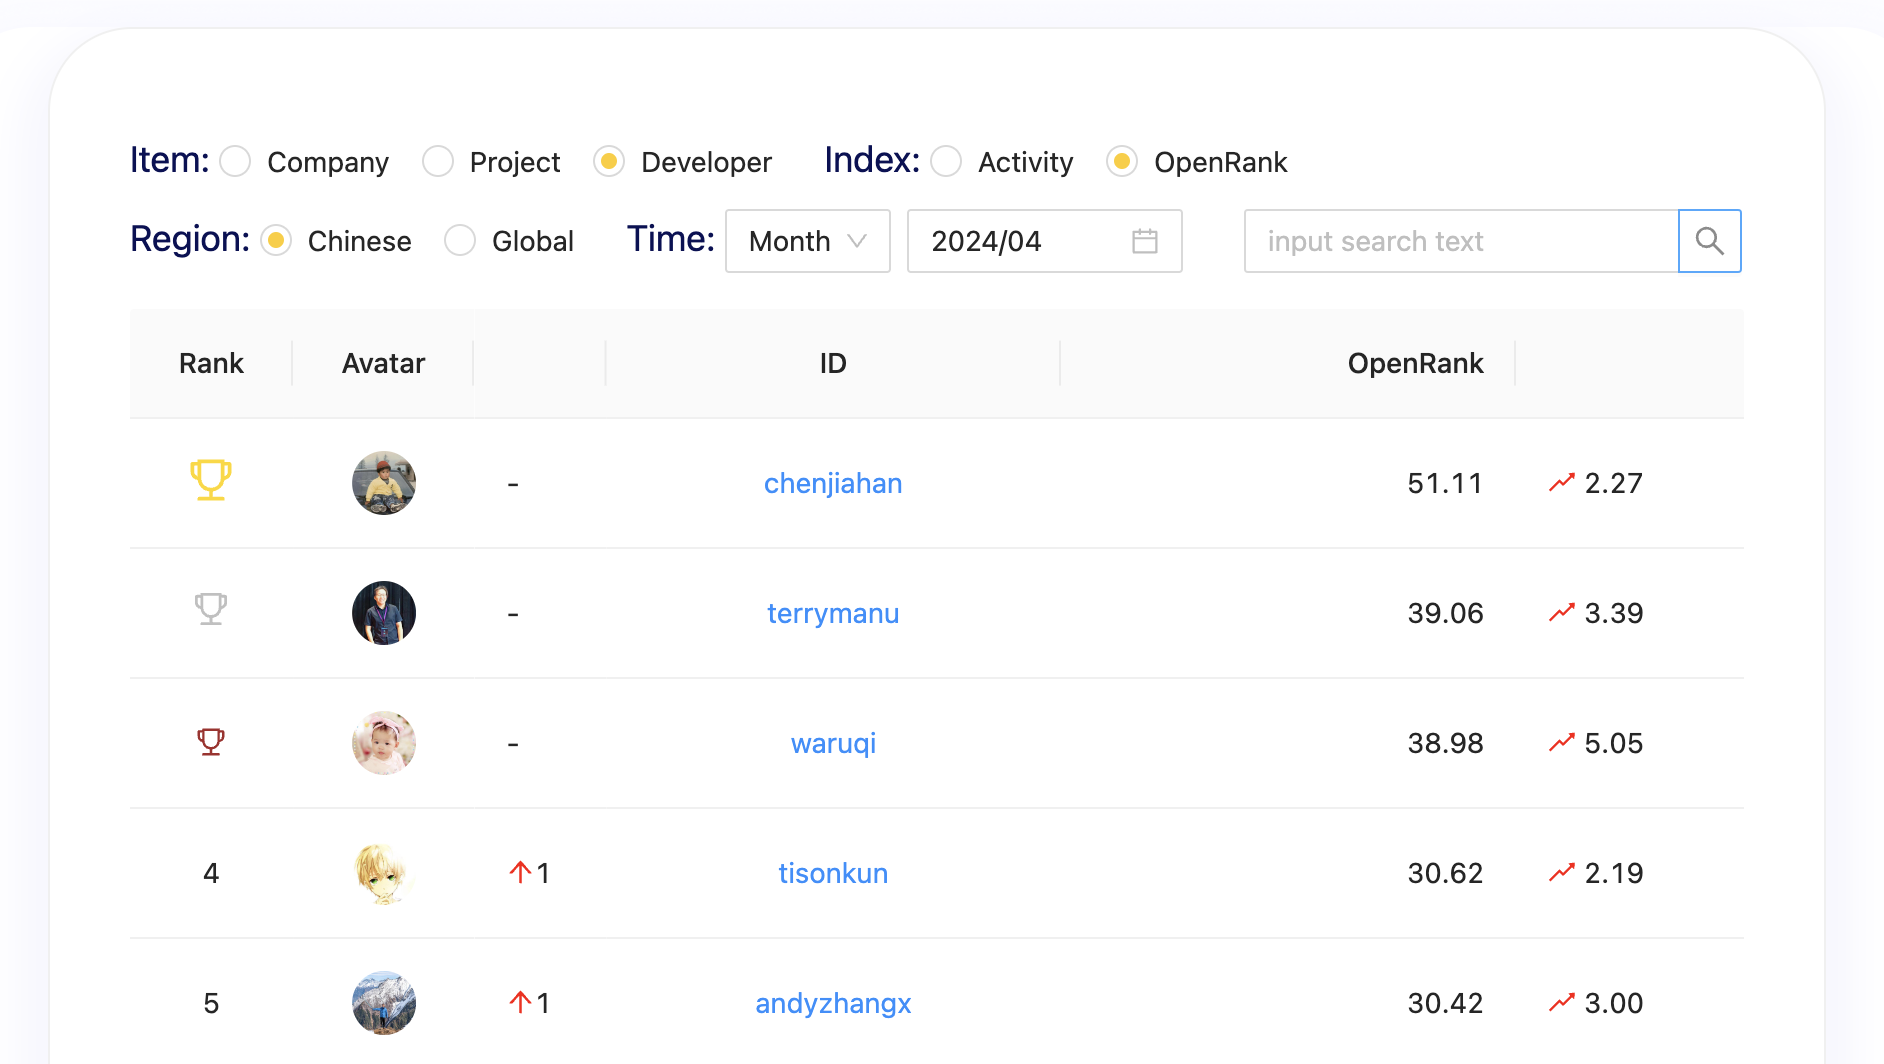
\includegraphics[width=0.85\linewidth]{figs/openrank.png}
    \caption{A screenshot of the interface of the OpenRank Leaderboard in May, 2024}
    \label{fig:openrank}
\end{figure}



Through the implementation of the OpenRank Leaderboard, the study found that developers were motivated to engage in more transparent communication, leading to improved collaboration behavior and a better community atmosphere. The leaderboard incentivized developers to make smaller, independent \ac{pr} and avoid direct commits to the repository, ultimately enhancing the quality of code contributions and fostering continuous improvement within the projects. The research also highlighted the role of the leaderboard in promoting healthy competition among developers, encouraging sustained engagement, and driving innovation within the open source projects.

The findings of the study indicated that the OpenRank Leaderboard effectively evaluates and steers developers' contributions, leading to positive behavioral changes and enhanced collaboration habits. Developers expressed a favorable perception of using graph network algorithms for contribution evaluation, with many acknowledging the alignment of rankings with their community perceptions and the value of combining results with community incentive operations. Overall, the study contributes valuable insights into the impacts and perceptions of using leaderboards as a gamification mechanism in company-led open source projects, emphasizing the importance of social network evaluation in motivating open source collaborations and driving innovation in software development.


\subsection{RQ3: Contribution barriers}

Beyond examining the motivations and social dynamics that propel developer participation in open-source projects, this research also delved into the barriers hindering their contributions. Through an analysis of five selected studies, several key challenges were identified that impede developer engagement and limit their ability to contribute effectively. The following sections will explore these barriers in detail, providing a comprehensive overview of the obstacles developers face in the open-source software development landscape. Based on a previous study by Mariam \citep{04guizani2021long}, the barriers to contribution were categorized into three main categories: technical challenges, social challenges, and process challenges. Each category encompasses distinct obstacles that hinder developer participation and require targeted interventions to overcome.


The chart \ref{fig:barriers} illustrates the obstacles individuals encounter when contributing to open source software projects which was found in 5 papers. The most frequent challenges revolve around social interaction, lack of timely responses or support, and technical difficulties, each occurring four times. Feeling intimidated or shy, cultural differences, and uncertainty about where to begin are also notable challenges, each happening twice. Other obstacles like submission procedures, governance compliance difficulties, unmet expectations, reception issues, inadequate or outdated projects, and prior technical experience are less common, each occurring once.

\begin{figure}[ht]
    \centering
    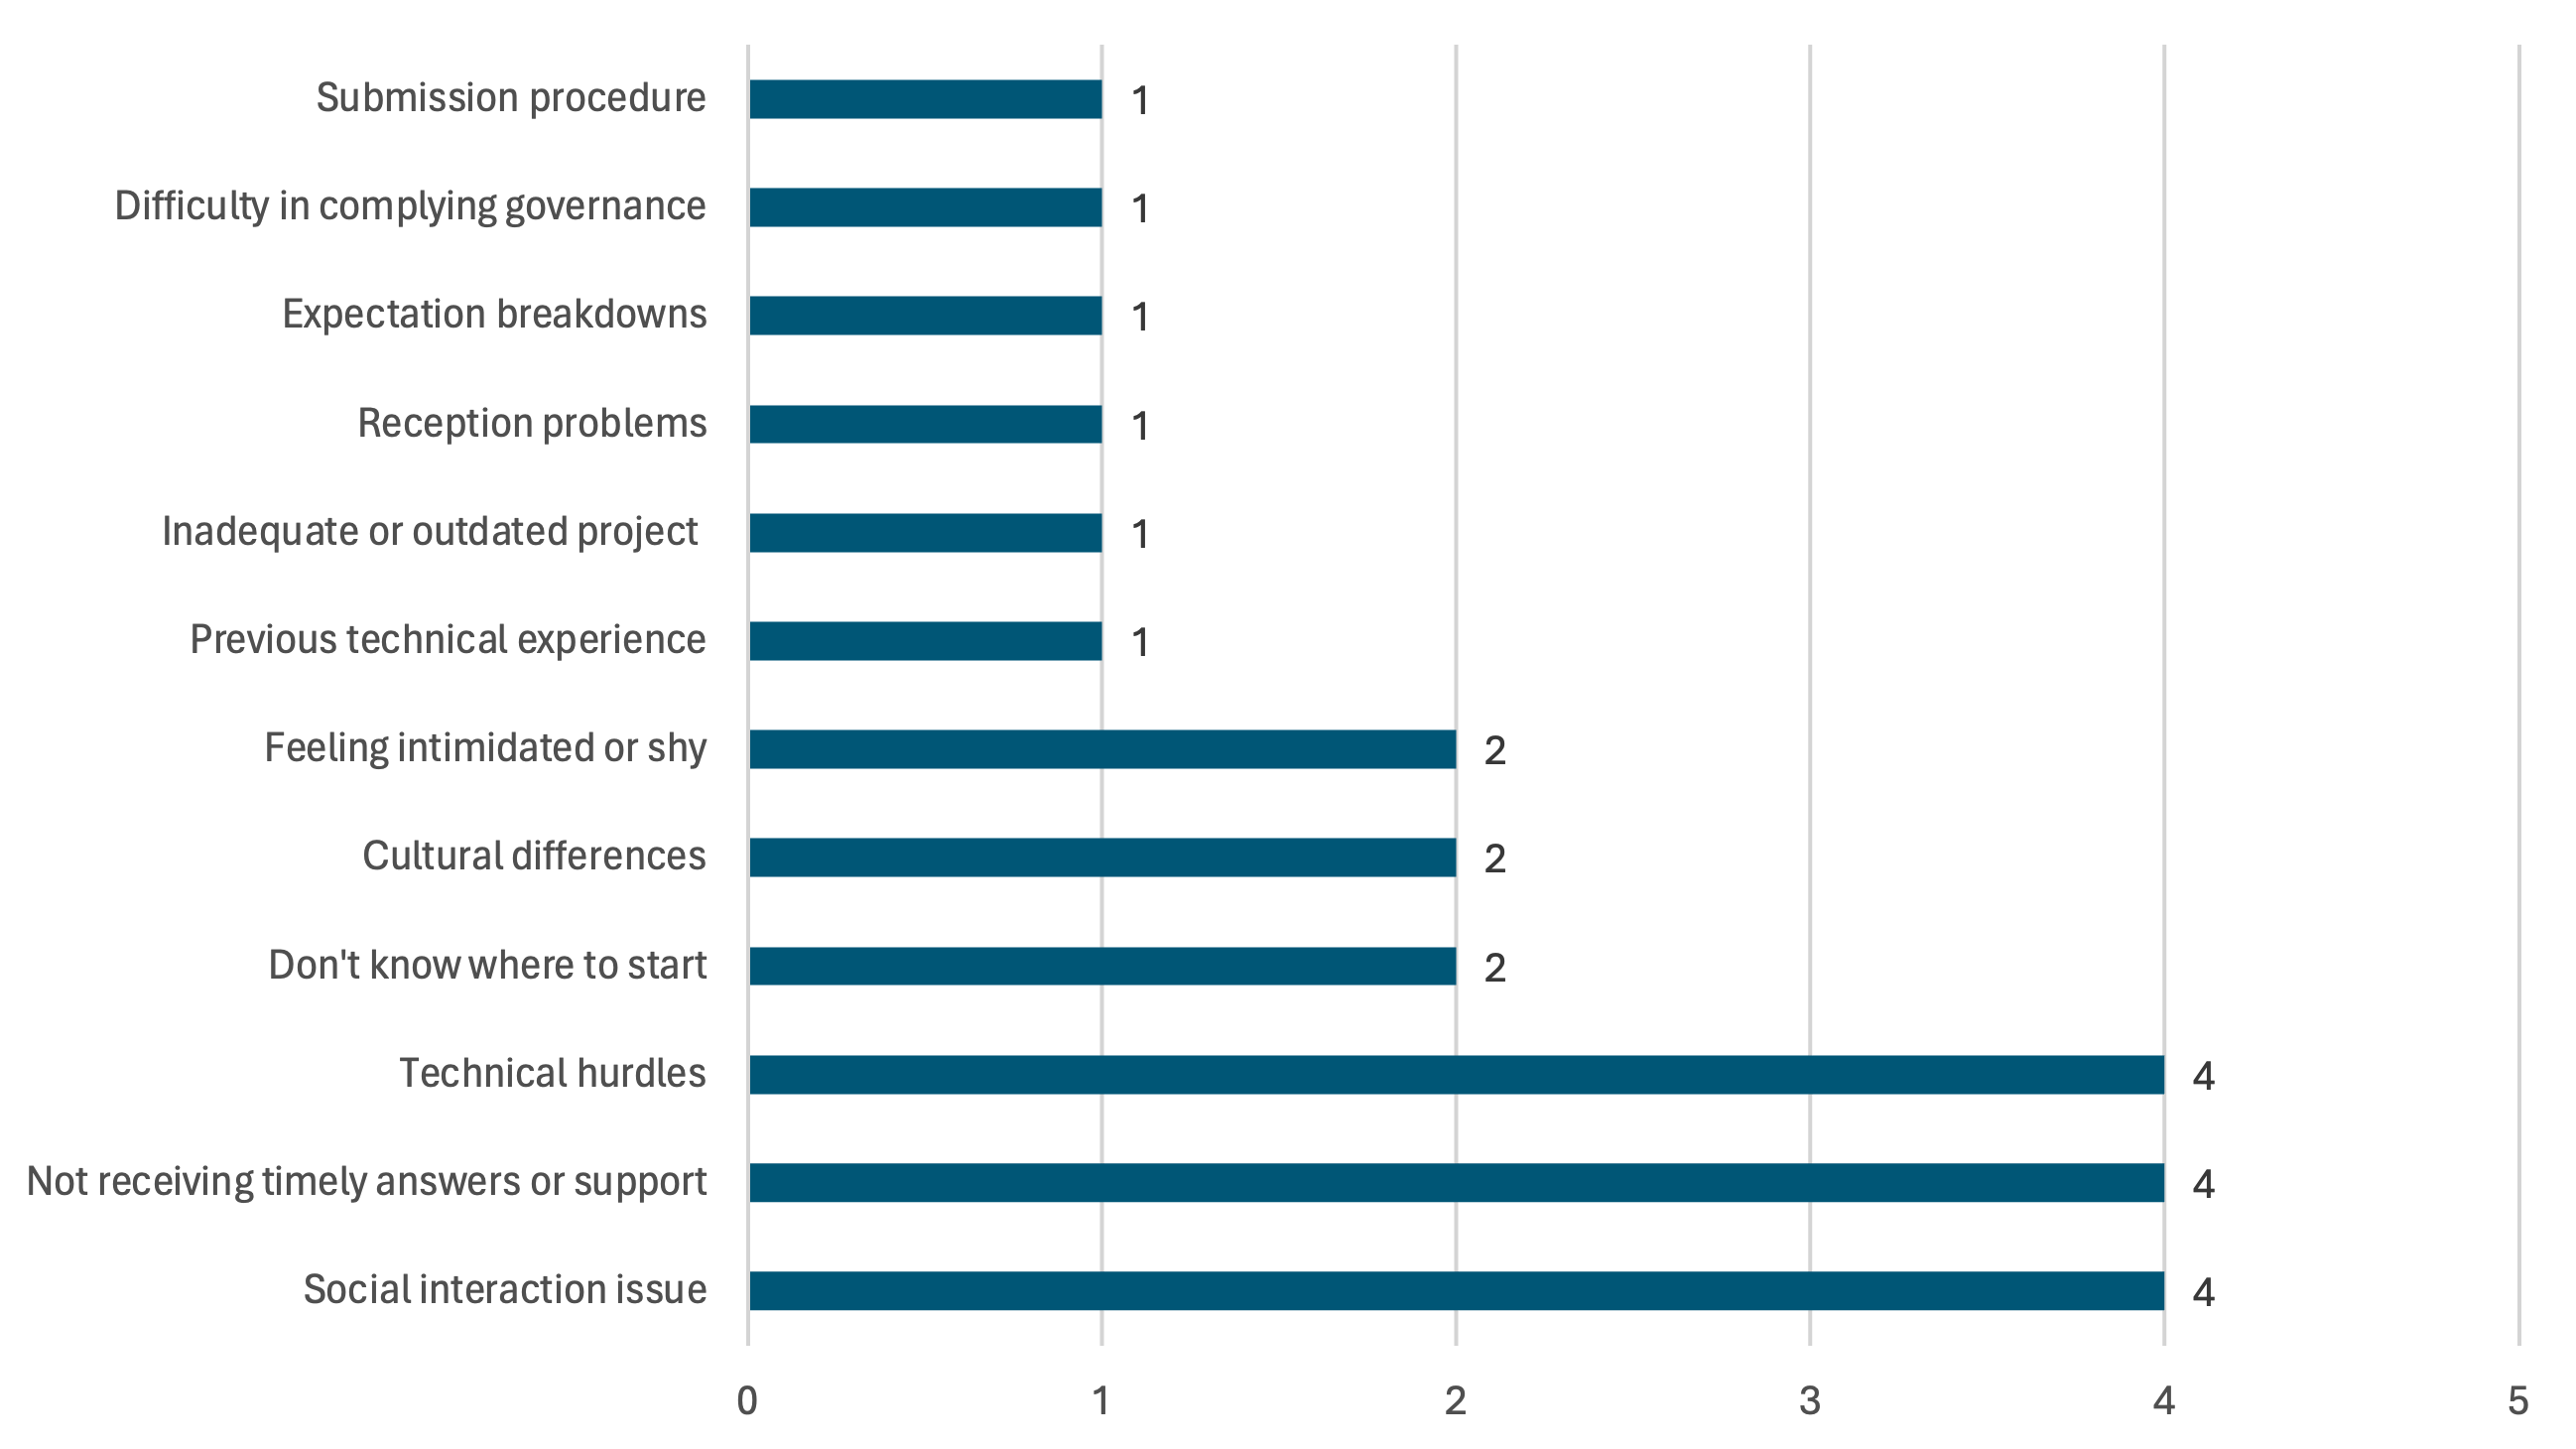
\includegraphics[width=1\linewidth]{figs/barriers.png}
    \caption{Barriers to contributing to open-source software projects}
    \label{fig:barriers}
\end{figure}



\subsubsection{Technical challenges}

A significant technical barrier to open-source contribution is the lack of technical background and domain expertise among potential contributors. Without a foundational understanding of the project's technological underpinnings, whether it's a specific programming language, framework, or software architecture, individuals may struggle to effectively engage and contribute to its development. Additionally, a lack of domain expertise in the subject matter the project addresses can hinder understanding of the problem space and the proposed solutions, making it difficult to provide meaningful contributions.

\begin{figure}[ht]
    \centering
    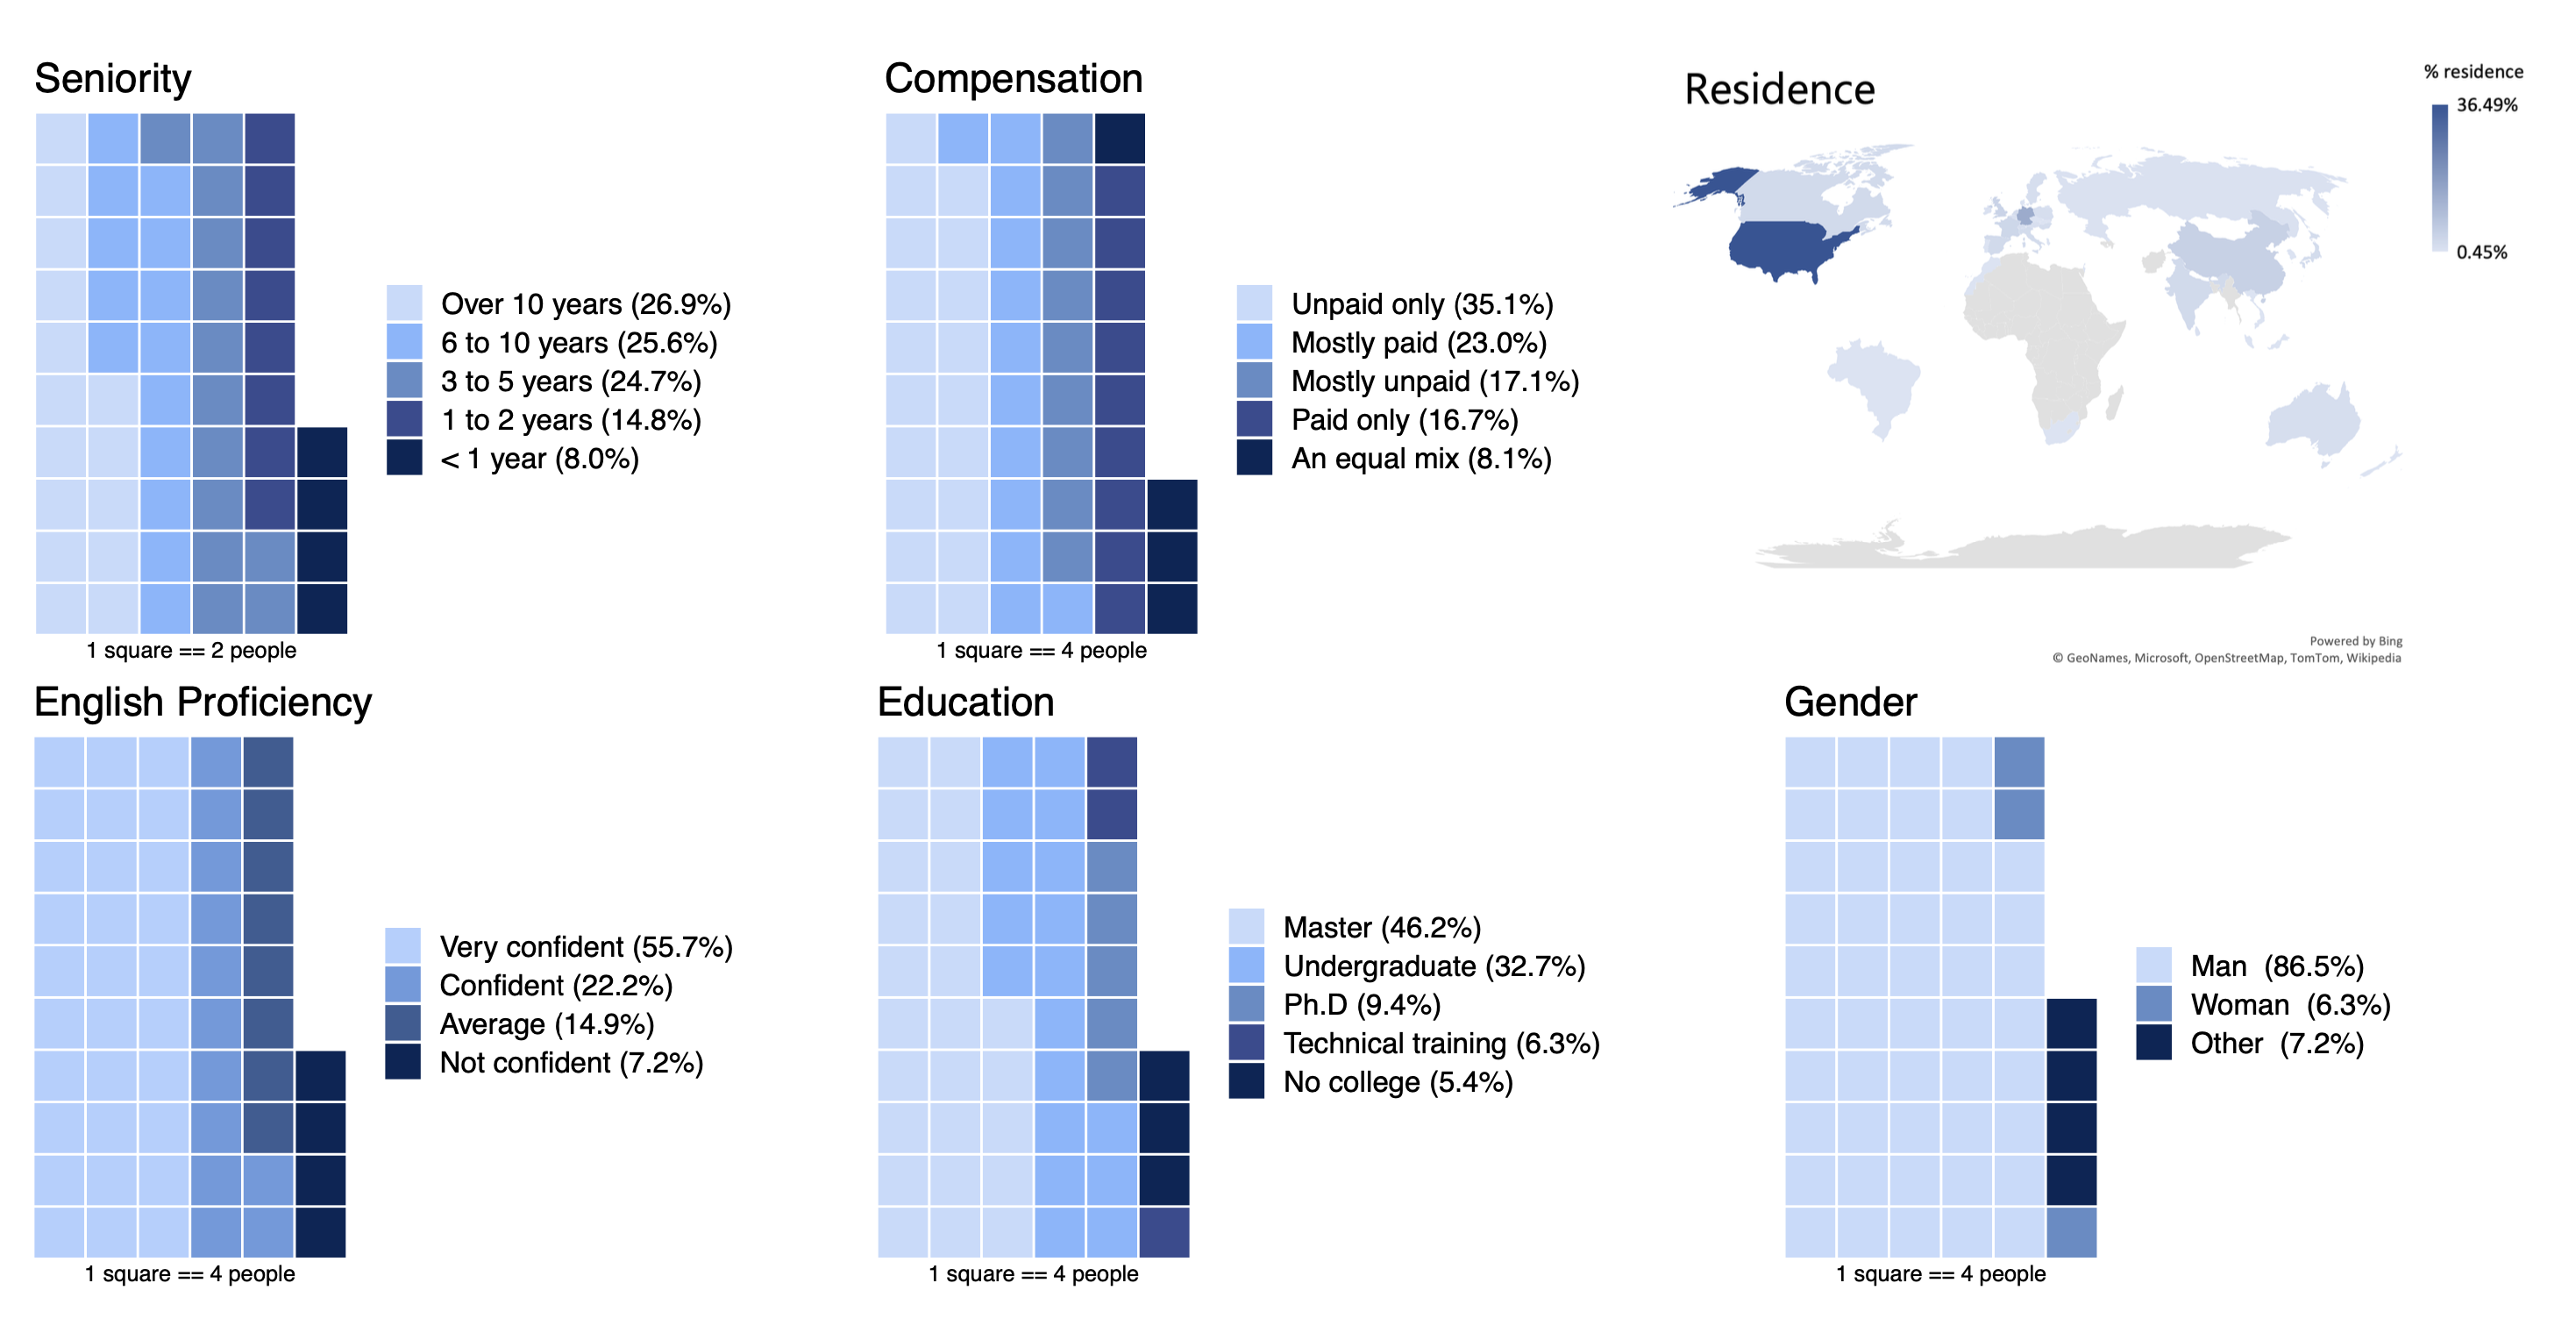
\includegraphics[width=1\linewidth]{figs/contributor_background.png}
    \caption{The background of the 223 developers from \ac{asf} \citep{04guizani2021long}}
    \label{fig:contributor_background}
\end{figure}

The diversity of programming languages used within and across open-source projects presents another challenge. Many projects utilize multiple languages for different components, and the open-source ecosystem as a whole encompasses a vast array of programming languages. Contributors often need to familiarize themselves with these languages to effectively understand and modify code, which can be daunting and time-consuming, particularly for those with limited programming experience or those accustomed to a single language.


Becoming a contributing member of an OSS project often entails acquiring project-specific skills, a process that can span months to a year. This temporal investment is highlighted in \citet{bird2007open} analysis of three OSS projects, where the median duration for newcomers to submit their initial patch and subsequently gain acceptance was revealed. This underscores the significant commitment required to successfully integrate into and contribute to OSS projects. The figure \ref{fig:timeskill} illustrates the time required to learn skills particular to a project, emphasizing the steep learning curve faced by newcomers.

\begin{figure}[ht]
    \centering
    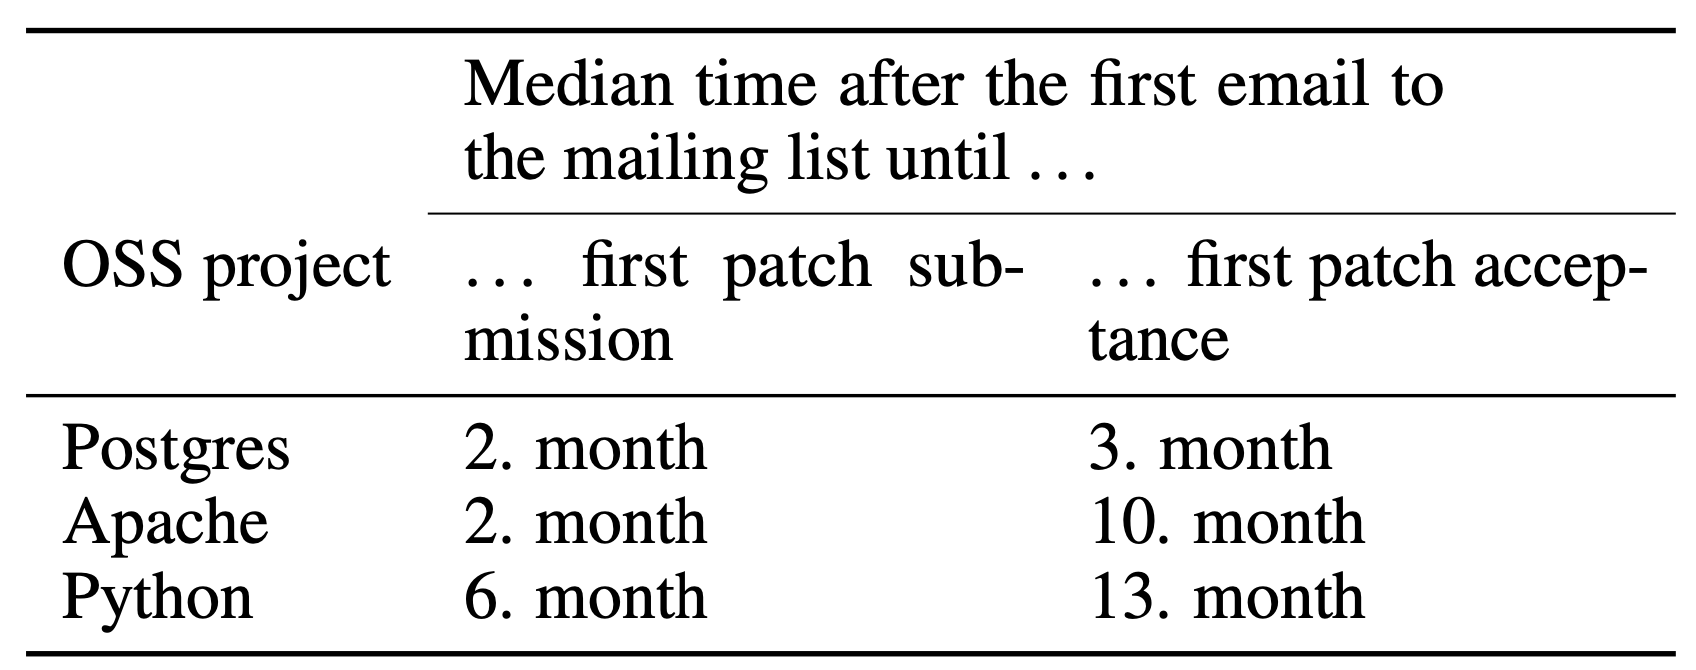
\includegraphics[width=0.65\linewidth]{figs/timeskill.png}
    \caption{Time required to learn skills particular to a project \citep{bird2007open}}
    \label{fig:timeskill}
\end{figure}

Discrepancies in technical skills and knowledge backgrounds among contributors can create a challenging environment for newcomers \citep{01steinmacher2015systematic,04guizani2021long}. Open-source projects often attract individuals with varying levels of expertise, from seasoned developers to those just starting their coding journey. Navigating a project with such diverse skill levels can be intimidating, making it difficult for newcomers to find their footing, ask questions without feeling inadequate, and contribute meaningfully \citep{14hannebauer2017relationship}.

Inadequate or outdated project documentation further compounds the challenges faced by contributors. Clear, comprehensive, and up-to-date documentation is crucial for understanding the project's codebase, workflow, and contribution guidelines. It serves as a roadmap for new contributors, guiding them through the project's intricacies. Without well-maintained documentation, newcomers may struggle to locate the correct areas for modification, understand the reasoning behind existing code, and follow established conventions, ultimately hindering their ability to contribute effectively to the project's development.



\subsubsection{Social challenges}

Effective communication is paramount in the open-source landscape, yet it is often fraught with challenges that can impede participation and collaboration. Limitations in the available communication tools, such as reliance on text-based platforms or asynchronous communication channels, can hinder real-time interaction and create misunderstandings. Additionally, diverse communication styles among members, ranging from direct and concise to more elaborate and nuanced, can lead to misinterpretations and impede the development of shared understanding. Moreover, conflicting viewpoints and disagreements within the community, while natural, can escalate into unproductive debates that alienate newcomers and create an unwelcoming environment \citep{02steinmacher2015social}.

% Image
\begin{figure}[ht]
    \centering
    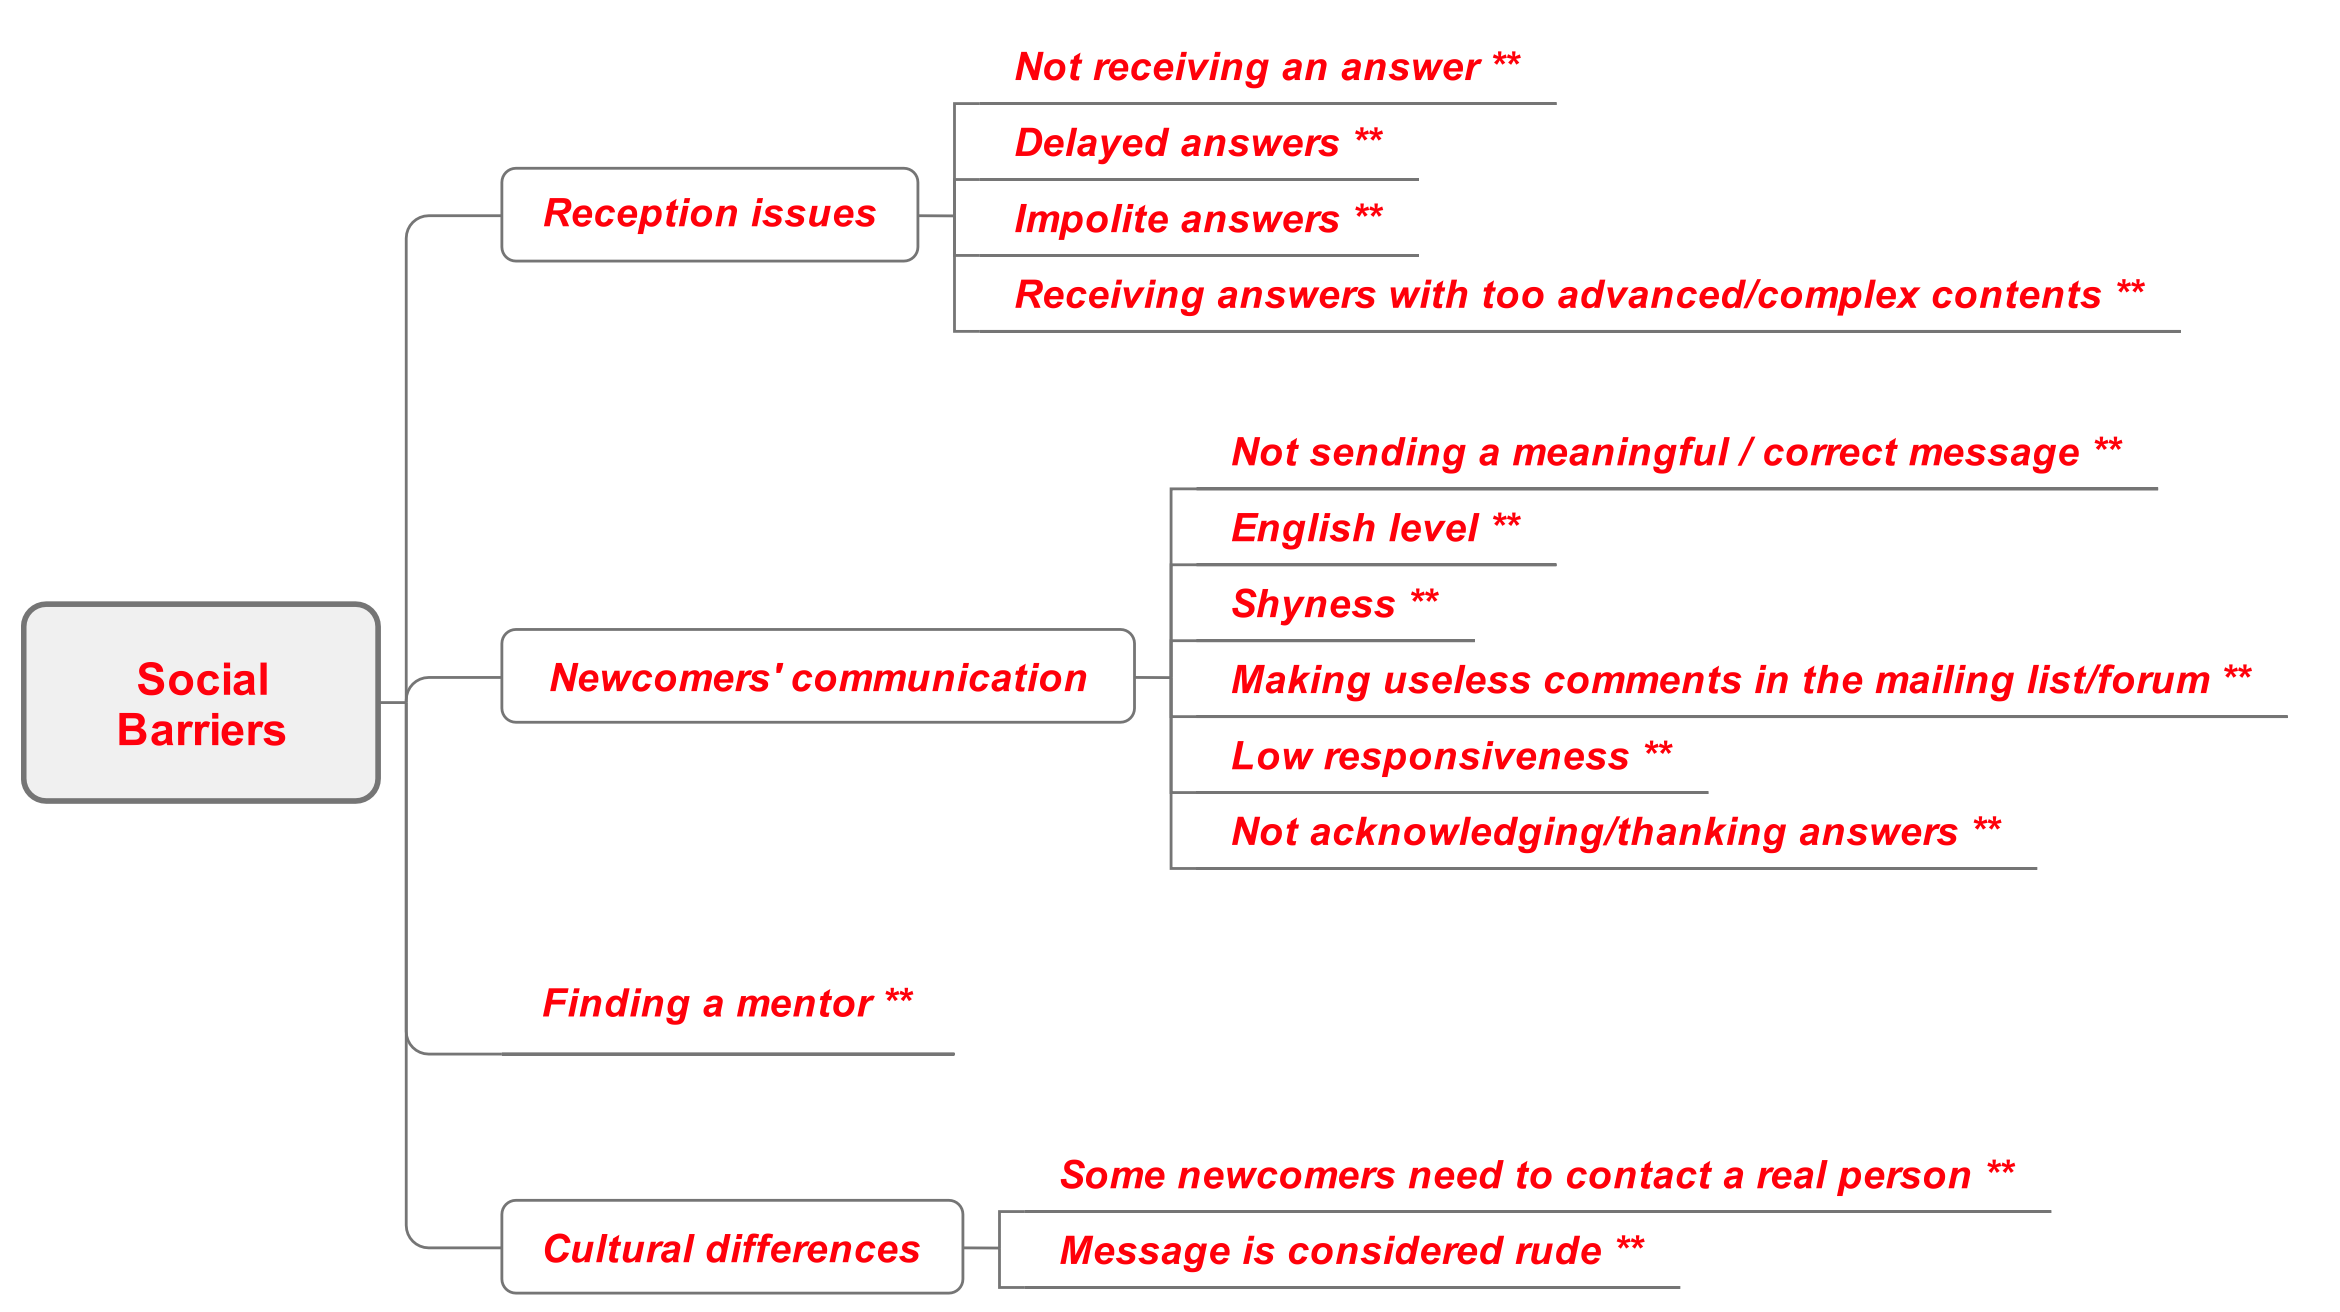
\includegraphics[width=1\linewidth]{figs/socialbarrier.png}
    \caption{Social barriers from Steinmacher's study \citep{03steinmacher2019overcoming}}
    \label{fig:socialbarrier}
\end{figure}

The social dimension of open-source projects is equally crucial, as it fosters a sense of belonging and encourages collaboration. However, newcomers often encounter difficulties establishing connections with project members, particularly in large and established communities. This can lead to feelings of isolation and a lack of mentorship or guidance, making it challenging to navigate the project's intricacies and identify suitable contribution opportunities. Moreover, if newcomers perceive a lack of responsiveness or support from existing members, their enthusiasm may wane, and they may ultimately abandon their efforts \citep{01steinmacher2015systematic,02steinmacher2015social,03steinmacher2019overcoming,04guizani2021long,14hannebauer2017relationship}.

The responsiveness of the community is a critical determinant of newcomers' experiences and long-term engagement. When individuals feel that their questions are ignored, their contributions are not acknowledged, or their efforts are not valued, they may become demotivated and disengage from the project. Conversely, timely feedback, recognition, and support can boost morale and encourage continued participation. Therefore, fostering a culture of responsiveness and inclusivity is essential for attracting and retaining new contributors.

Cultural aspects, often overlooked but equally significant, can also create barriers for newcomers seeking to integrate into the project community. Different cultural backgrounds and norms can lead to varying expectations regarding communication styles, decision-making processes, and interpersonal interactions. These differences can create misunderstandings and misinterpretations, hindering the establishment of rapport and trust between newcomers and existing members. Additionally, the initial reception and onboarding process for newcomers can significantly impact their experience and willingness to contribute. A welcoming and supportive environment, with clear guidelines and mentorship opportunities, can make a substantial difference in fostering a sense of belonging and encouraging long-term participation.


\subsubsection{Process challenges}

Embarking on a journey to contribute to open-source projects can often feel like navigating a complex maze. The path is riddled with challenges, particularly for newcomers who are unfamiliar with the unique ecosystem of each project. Understanding the specific workflow, which can vary significantly between projects, is a critical first step. This includes grasping the nuances of branching strategies, pull request etiquette, and the overall development cycle. Additionally, mastering version control systems like Git, with its array of commands and concepts, can be a steep learning curve.

\citet{04guizani2021long} highlighted significant process challenges faced by developers contributing to \ac{asf} projects. The research revealed that developers encounter complexities in understanding and following the contribution process, from becoming a committer to getting their contributions accepted. Additionally, the study identified the process of adding new committers as bureaucratic and tedious, further complicating the onboarding experience. These process challenges are illustrated in figure \ref{fig:processChallenges} along with other barriers faced by developers contributing to ASF projects.

\begin{figure}[ht]
    \centering
    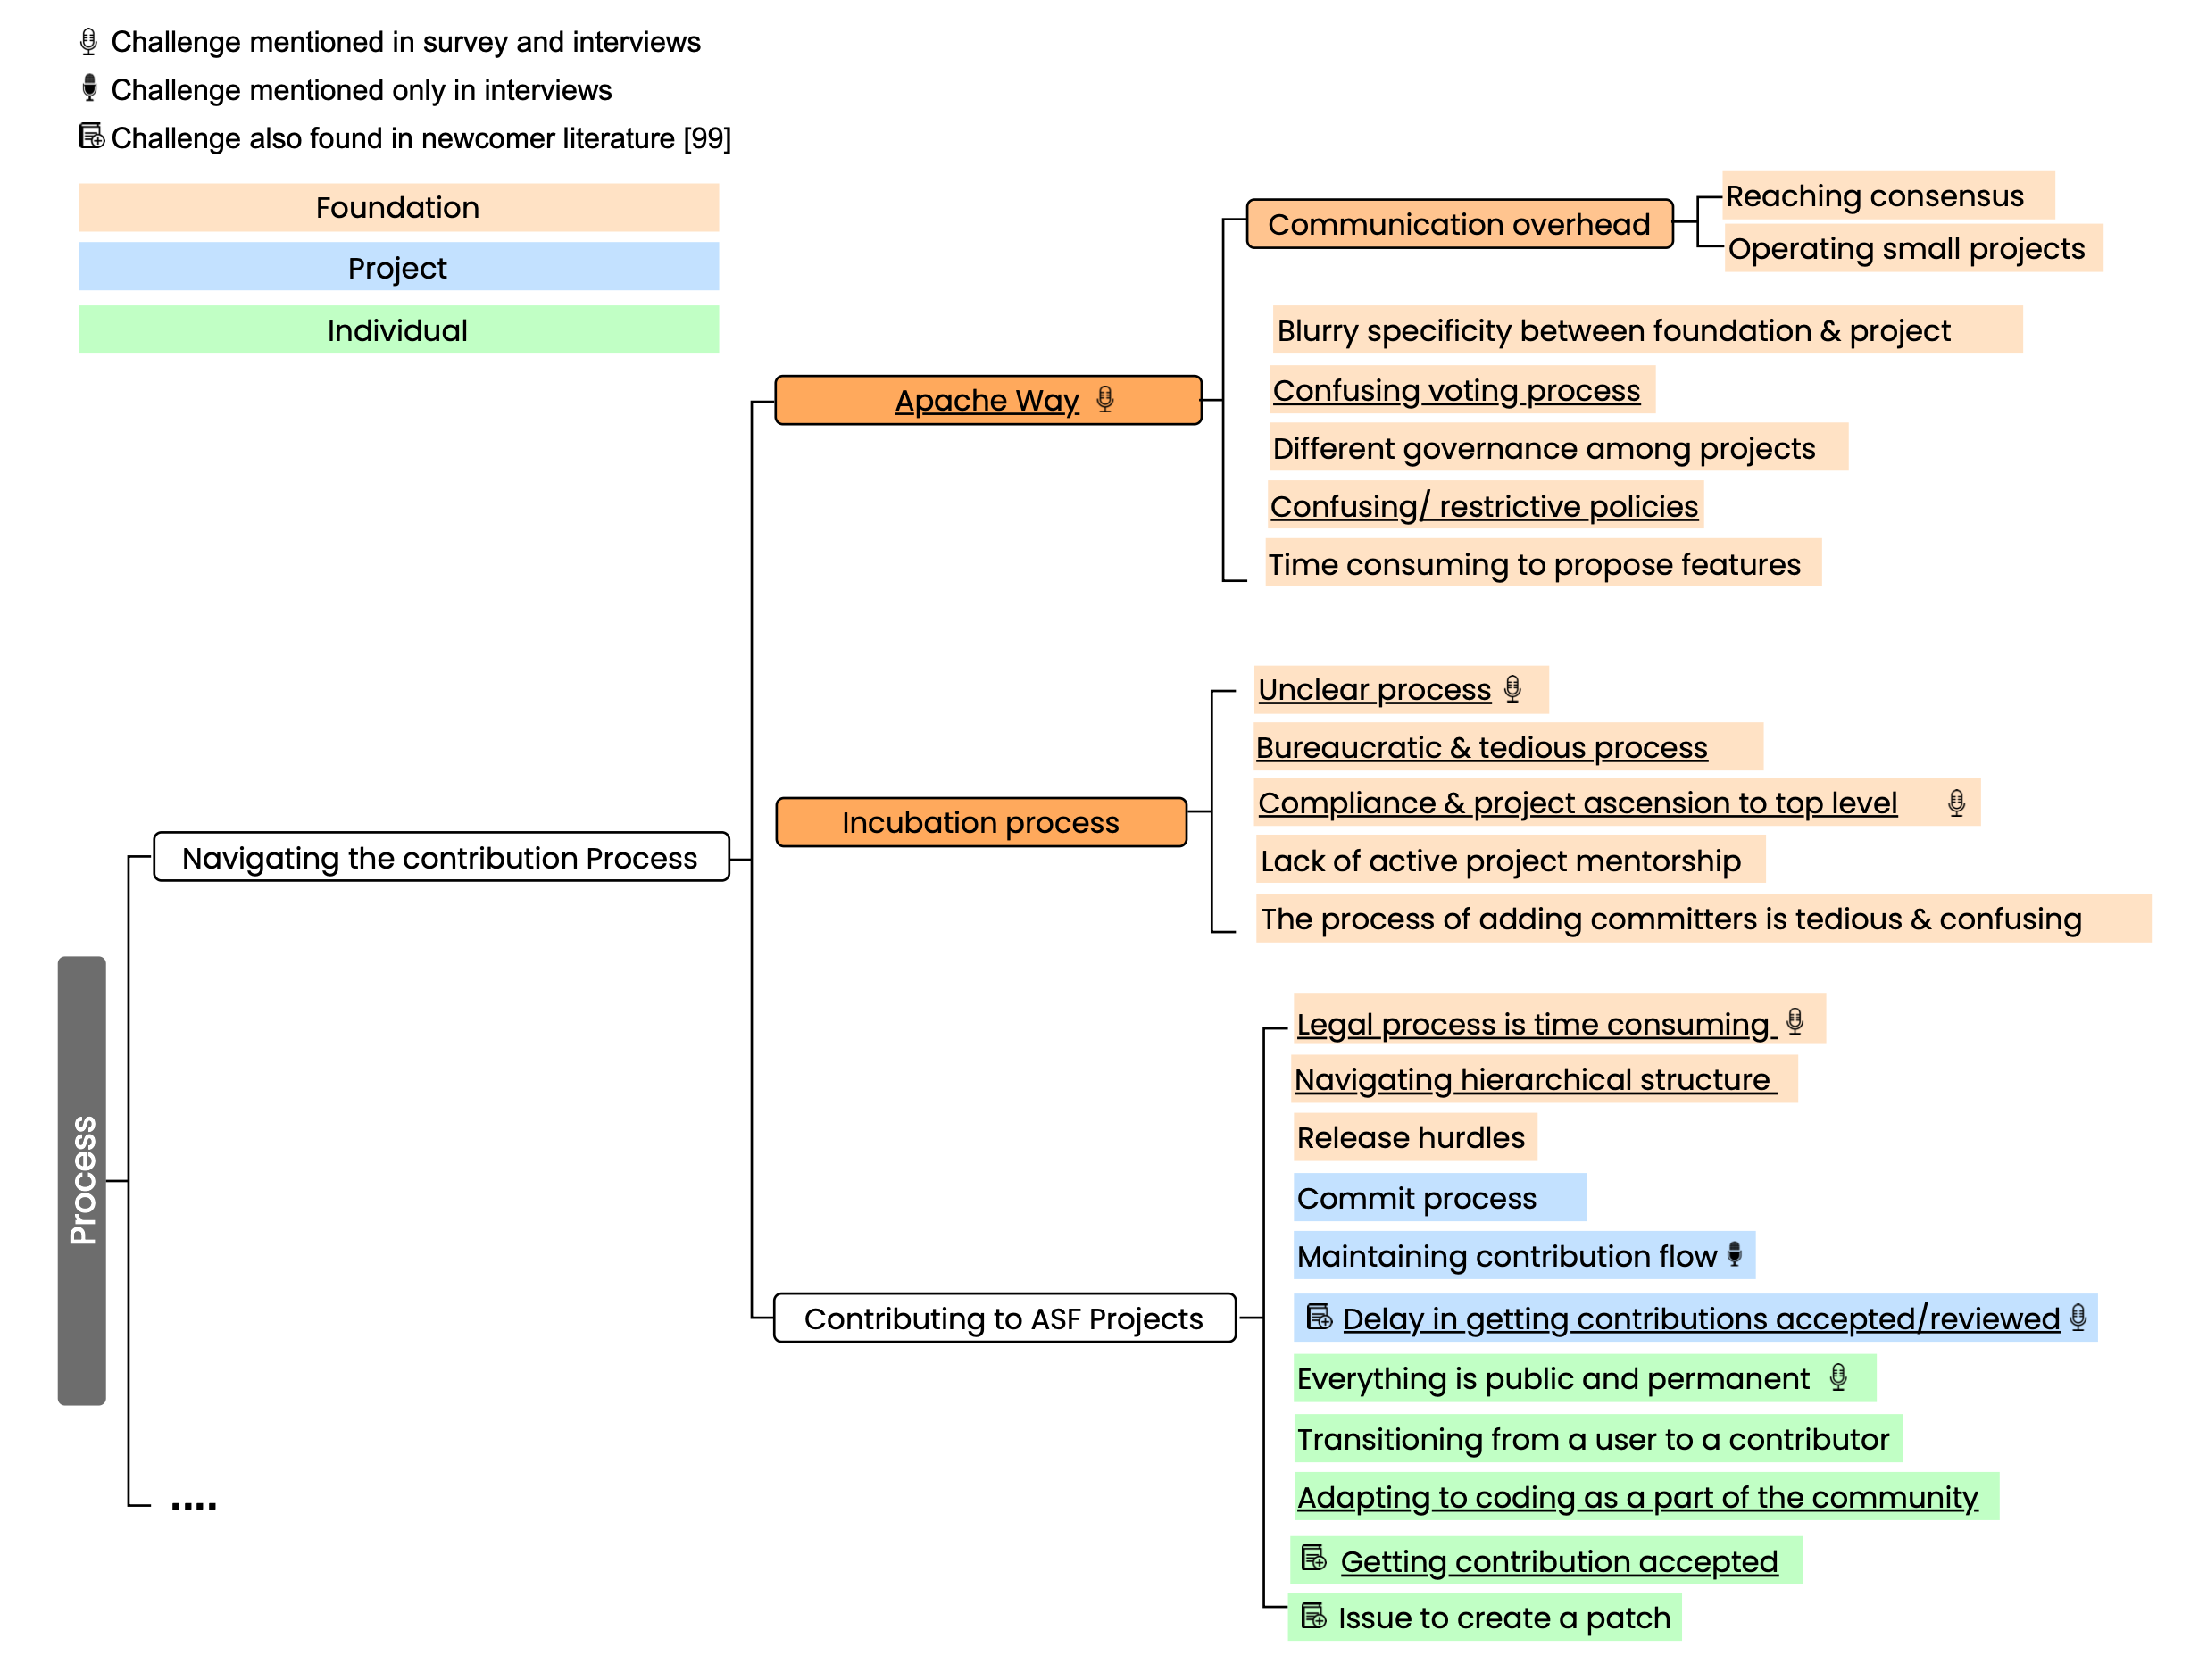
\includegraphics[width=1\linewidth]{figs/processChallenges.png}
    \caption{Challenges faced by developers contributing to ASF projects \citep{04guizani2021long}}
    \label{fig:processChallenges}
\end{figure}


In corporate settings, product development teams often adhere to a rigid process, like Agile or Scrum, with clear roles, responsibilities, and hierarchies. Conversely, open-source projects operate more flexibly, with contributors often taking on diverse roles. This lack of formal structure can be challenging for newcomers, who may find it difficult to identify decision-makers, understand governance, or navigate informal power dynamics within the community.


Adherence to coding standards and contribution guidelines is another significant hurdle. Each project has its own meticulously crafted conventions and best practices, often accumulated over years of development. Failing to comply with these standards can lead to rejected contributions or frustrating delays in getting changes merged. For newcomers, who are still acclimating to the project's culture and technical requirements, this can be a discouraging experience.

Compounding these challenges is the frequent lack of comprehensive and user-friendly onboarding materials. While some projects may boast extensive documentation, it is often not tailored for newcomers or may be outdated, leaving crucial information buried or irrelevant. The absence of step-by-step tutorials that walk newcomers through the contribution process, clear explanations of the project's architecture and codebase, or readily available mentorship programs can leave them feeling lost and overwhelmed. This lack of guidance not only discourages potential contributors but also hinders their ability to make meaningful contributions, ultimately depriving the project of valuable talent and fresh perspectives.

Moreover, developers may find certain open-source projects terrifying due to their immense scale and intricacy. With vast codebases, numerous contributors, and a long history of development, it can be difficult to know where to start or how to make a meaningful impact. The lack of a structured onboarding process, coupled with the fear of making mistakes or not understanding the project's intricacies, can create a sense of paralysis and prevent newcomers from taking that crucial first step.



\clearpage               % Add chapter 5
%% reference list
\phantomsection     % this command ensures the internal links will be correct
\printbibliography[heading=bibintoc,title={References}] % Prints reference list
\label{myLastPage}
\clearpage % This command will start the next section from the new page

        % Add references

%%%%%%%%%%%%%%%%%%%
%% Appendix section starts here
%%%%%%%%%%%%%%%%%%%
\addtocontents{toc}{\cftpagenumbersoff{section}} % Add "Appendices" to table of content without page number
% Modify the section heading to contain "Appendix" at the beginning
\titleformat{\section}
{\Large}
{Appendix \thesection}{1em}{}

% Appendices
\begin{appendices}
  \renewcommand{\thesection}{\arabic{section}}    % Numbering style
  %% Appendix 2
\pagenumbering{arabic}  % This will reset the page numbering
%\thispagestyle{empty} % use this if page number needs to be removed

\begin{landscape}


  \section{Selected articles and papers for SLR}\label{App:A}

  \begin{center}

    \begin{longtable}{ | m{5em} | m{25em}| m{22em} | m{4em} | }
      \caption{Articles and papers selected for SLR.\label{articles}}                                                                                                                                                                                                                      \\

      \hline
      Article ID & Title                                                                                                                                         & Authors                                                                                                         & Y.O.P \\ \hline
      A01        & A systematic literature review on the barriers faced by newcomers to open source software projects                                            & Steinmacher, I., Silva, M. A. G., Gerosa, M. A., \& Redmiles, D. F.                                             & 2015  \\ \hline
      A02        & Social barriers faced by newcomers placing their first contribution in open source software projects                                          & Steinmacher, I., Conte, T., Gerosa, M. A., \& Redmiles, D.                                                      & 2015  \\  \hline
      A03        & Overcoming social barriers when contributing to open source software projects                                                                 & Steinmacher, I., Gerosa, M., Conte, T. U., \& Redmiles, D. F.                                                   & 2019  \\ \hline
      A04        & The long road ahead: Ongoing challenges in contributing to large oss organizations and what to do                                             & Guizani, M., Chatterjee, A., Trinkenreich, B., May, M. E., Noa-Guevara, G. J., Russell, L. J., ... \& Sarma, A. & 2021  \\ \hline
      A05        & Intrinsic motivation in open source software development                                                                                      & Bitzer, J., Schrettl, W., \& Schröder, P. J.                                                                    & 2007  \\ \hline
      A06        & Toward an understanding of the motivation of open source software developers                                                                  & Ye, Y., \& Kishida, K.                                                                                          & 2003  \\ \hline
      A07        & OpenRank Leaderboard: Motivating Open Source Collaborations Through Social Network Evaluation in Alibaba                                      & Zhao, Shengyu                                                                                                   & 2024  \\ \hline
      A08        & How Are Paid and Volunteer Open Source Developers Different? A Study of the Rust Project                                                      & Zhang, Yuxia                                                                                                    & 2024  \\ \hline
      A09        & Why hackers do what they do: Understanding motivation and effort in free/open source software projects                                        & Lakhani, K. R., \& Wolf, R. G.                                                                                  & 2005  \\ \hline
      A10        & An empirical analysis of open source software developers' motivations and continuance intentions                                              & Wu, C. G., Gerlach, J. H., \& Young, C. E.                                                                      & 2007  \\ \hline
      A11        & The shifting sands of motivation: Revisiting what drives contributors in open source                                                          & Gerosa, M., Wiese, I., Trinkenreich, B., Link, G., Robles, G., Treude, C., ... \& Sarma, A.                     & 2021  \\ \hline
      A12        & The characteristics and motivations of library open source software developers: An empirical study                                            & Choi, N., \& Pruett, J. A.                                                                                      & 2015  \\ \hline
      A13        & Leadership characteristics and developers' motivation in open source software development                                                     & Li, Y., Tan, C. H., \& Teo, H. H.                                                                               & 2012  \\ \hline
      A14        & On the relationship between newcomer motivations and contribution barriers in open source projects                                            & Hannebauer, C., \& Gruhn, V.                                                                                    & 2017  \\ \hline
      A15        & Understanding the motivations, participation, and performance of open source software developers: A longitudinal study of the Apache projects & Roberts, J. A., Hann, I. H., \& Slaughter, S. A.                                                                & 2006  \\ \hline
      A16        & Motivations for participating in open source software communities: Roles of psychological needs and altruism                                  & Ke, W., \& Zhang, P.                                                                                            & 2008  \\ \hline
      A17        & Working for free? Motivations for participating in open-source projects                                                                       & Alexander Hars, S. O.                                                                                           & 2002  \\ \hline
      A18        & Exploring motivations for contributing to open source initiatives: The roles of contribution context and personal values                      & Oreg, S., \& Nov, O.                                                                                            & 2008  \\ \hline
      A19        & Community dynamics in open source software projects: Aging and social reshaping                                                               & Hannemann, A., \& Klamma, R.                                                                                    & 2013  \\ \hline
      A20        & The material and social dynamics of motivation: Contributions to Open Source language technology development                                  & Freeman, S.                                                                                                     & 2007  \\ \hline
    \end{longtable}
  \end{center}
\end{landscape}

\clearpage % This command will start the next section from the new page            % Add appendix 1
  % %% Appendix 2
\pagenumbering{arabic}  % This will reset the page numbering
%\thispagestyle{empty} % use this if page number needs to be removed
\section{References}\label{App:B}

The text must include references to the sources you use. LUT University applies the Harvard referencing style, also called the author-date style, with in-text referencing and a detailed reference list at the end.

The purpose of a reference list is to provide sufficient information on a source used in the study, allowing the reader to consult the original source for further information. The reference enables the reader to find detailed information on the source easily in the list of references. You should refer to the original and most recent sources. If no new studies have been published on the topic in question, also older ones may be used.

Referring to a source means that you explain the contents of the source material in your own words. Direct citations, on the other hand, are placed inside quotes \enquote{Quote}. Plagiarism or using another person’s original material without appropriate referencing is not allowed.

\subsection*{Referencing technique}

In the Harvard system, the citation is placed in parentheses directly in the text to indicate the passage that has been cited from another source. Place the citation before the period that ends the sentence when it refers only to the sentence in question \citep{CitekeyInbook2}. If you are referring to more than that one sentence, introduce the source you are summarizing or paraphrasing at the beginning of the paragraph. Then, refer back to the source when needed to ensure your reader understands you are still using the same source. In-text references, specifying page numbers, are not used unless a specific part of the text is directly referred to or it is a direct quotation. Please note that the author does not always have to be an individual but can also be, for example, an organization. If the publication's author does not appear in the source, the name of the publication is referred to instead of the author's name.

\subsubsection*{Author's name cited in the text (direct)}
Direct citation is used when the author’s name(s) is a part of the sentence structure, with the year in parentheses. The following is obtained by using \verb+\citet{key}+ command.
\begin{quote}
\citet{All87} claims that \ldots
\end{quote}
More than three authors for a work
\begin{quote}
\citet{CHOWDHURY} in their work \ldots
\end{quote}
On some special occasions, all the authors (more than three) can be cited, but this form should be considered only at the \emph{special} case by using \verb+\citet*{key}+ command
\begin{quote}
\citet*{Biz98} showed \ldots
\end{quote}

\subsubsection*{Author's name not cited in the text (indirect)}
Indirect citation is used when the author's name(s) is not mentioned directly in the sentence structure. The indirect citation will appear at the relevant point in the sentence or at the end of the sentence in parentheses. The following is obtained by using \verb+\citep{key}+ command.

\begin{quote}
Earlier research claims that \ldots \citep{Sav92}.
\end{quote}
Two authors with postnote
\begin{quote}
At the theoretical approaches of \ldots \citep[102]{All87}.
\end{quote}
More than three authors for a work
\begin{quote}
\ldots, \citep{VELEVA}.
\end{quote}
Combined citation with three entries using the command \verb+\citep{key1,key2,key3}+
\begin{quote}
According to previous studies, the presented conclusions are consistent \citep{Mil97,Dal05,All87}.
\end{quote}

In many situations, it is justified to combine the content of several sources, and then it is recommended to use content-specific indirect references. For example, in the following way:
\begin{displayquote}[{\cite{Talikka}}][]
In literature we can find challenges relating to a wide variety of issues including environmental sustainability \citep{DAGILIUTE}, business needs \citep{VELEVA}, food production \citep{CHOWDHURY}, urban development \citep{Joss,swapan,freeman,WAITE}, and education \citep{ZIDANSEK,Biberhofer}.
\end{displayquote}

A wide variety of sources can be used in the text. In addition to the above, Master's theses \citep{Hyv19}, websites \citep{CitekeyMisc}, interviews \citep[interview 6.6.2007]{CitekeyMisc2}, technical reports \citep{Lai09}, booklets \citep{CitekeyBooklet}, manuals \citep{CitekeyManual}, proceedings \citep{CitekeyProceedings}, standards \citep{standardi}, patents \citep{US5503249} or AI-language models \citep{ChatGPT} can be used.

All the bibliography information is given in the References. If you refer several works published by the same author in the same year, add lowercase letters (a, b, c…) after the publication year to distinguish the sources. Use the same alphabetical notation also in the list of references. There are several referencing and citation styles. It is essential to use the same style throughout the thesis consistently. Examples and detailed instructions on referencing:
\begin{itemize}
    \item \href{https://libguides.lut.fi/citingelectronicdocuments}{\textcolor{blue}{LUT Academic Library’s instructions}} on how to cite electronic documents
    \item \href{https://libguides.aalto.fi/citation_guide}{\textcolor{blue}{Aalto University citation guide}}
    \item \href{https://www.librarydevelopment.group.shef.ac.uk/referencing/harvard.html}{\textcolor{blue}{Harvard referencing}}, University of Sheffield 
\end{itemize}

\clearpage % This command will start the next section from the new page            % Add appendix 2
  % %% Appendix 3
\pagenumbering{arabic}  % This will reset the page numbering
%\thispagestyle{empty} % use this if pagenumber needs to be removed
\section{Tables, figures, equations, numbers, symbols, and abbreviations }\label{App:C}

It is a good idea to illustrate your text with figures and tables. Figures and tables must have captions and consecutive numbering. The captions of tables are placed above the table, and those of figures are below the figure. Refer to the figures and tables in the text body, preferably before you introduce them, and align them with the text body. In many theses, the alignment of figures and tables has been centered and without wrapping text around them, but the author can select the formatting options as long as they are coherent in the whole work. \LaTeX~ tries to place all floating objects (figures and tables) at the top of the page or in the best place and to avoid multiple floating objects on the same page. Because of this, for several floating objects in series, their position can be shifted several pages forward. It is also possible for floating objects to move to the next section. Because of this, several consecutive floating objects should be avoided, and enough text should be added between the floating objects. In this template \verb|\usepackage[section]{placeins}| setting is used to force floating objects to stay in the appearing section. You can also use \verb|\FloatBarrier| command to set a position limit for floating objects.

Remember to add alt text (alternative text) to your figures and tables to ensure accessibility. Alt text is read by a designated reader and can be viewed even when the image cannot be displayed on the page. In \LaTeX~the alt text has to be set manually and you should make sure it describes the object sufficiently and understandably. You can add the alt text by using the command \verb|\pdftooltip{Object}{Alt-text}|.

\subsection*{Tables}
Give your table number and caption, and refer to them in the text. Place the caption above the table, name its columns, and mention the units applied, as in Table \ref{tab:1} below. Avoid empty columns or rows. The recommended font size is 10.

\begin{table}[!h]
    \centering
    \caption{Sensor measurements.}
    \pdftooltip{\begin{tabular}{|c|c|}
        \hline
        Voltage $U$ [V] & Pressure $p$ [Pa] \\
        \hline\hline
        0.984 & 0 \\
        2.252 & 150 \\
        2.772 & 300 \\
        3.181 & 450 \\
        3.615 & 600 \\
        3.817 & 750 \\
        4.088 & 900 \\
        \hline
    \end{tabular}}{Example of table layout. In the table, the presentation of sensor measurement data is presented. Data includes measured voltage and pressure pairs for seven individual measurements.}
    \label{tab:1}
\end{table}

\section*{Figures, charts, graphic elements}
Images help illustrate your text. The text should contain a reference to every figure. Number your figures and place a caption underneath – not inside the figure.

You should use a software program like Excel or Matlab to draw charts. Charts should be clear and easy to understand. Use a white background. A background grid is allowed if it does not make the figure difficult to interpret. Variables and measurement points should be clearly visible. Name the axes and their units. An example script to produce a Figure \ref{fig:1} with Matlab is presented in Appendix \ref{App:E}. To maintain full accessibility of the document, you should use embedded fonts in the vector figures. The example script will not produce a figure with embedded fonts, and the jpg or png formats would be better with respect to document accessibility. However, the figure quality is reduced.

\begin{figure}[!h]
   \centering
    \pdftooltip{\includegraphics[width=.5\textwidth]{figs/example_name.pdf}}{Example result figure produced by Matlab software. The figure illustrates the sine function in a range from 0 to three pi. The scaling of font size from the original 18pt to the thesis size of approximately 12pt is illustrated.}
    \caption{Illustration of Matlab example figure.}
    \label{fig:1}
\end{figure}

Create as many of the figures yourself as you can. Use the same font as in the text body and equations. Try to maintain the font size in the figure as close as possible to the main text font size. If you use images created by someone else, remember to cite them correctly. Remember that images are copyrighted works, the use of which must always be authorized by the author. Captions need to be in the same language as the text body.

Figure \ref{fig:2} shows a gas fermenter in a laboratory configuration. The image is positioned at the beginning of the page, and with the command \verb|\FloatBarrier|, the following text is forced to appear after the image.

\begin{figure}[t]
   \centering
    \pdftooltip{\includegraphics[width=.5\textwidth]{figs/Picture1.png}}{Example picture of the gas fermentor. The picture illustrates the test equipment and measurement arrangements in the laboratory.}
    \caption[Short description for List of Figures]{Gas fermentor (VTT 2020, LUT image bank).}
    \label{fig:2}
\end{figure}
\FloatBarrier

Do not end a paragraph in a figure or table. Add text underneath, such as comments on the figure. Large figures, tables, long equations, and other supporting material can be appended.

\subsection*{Numbers, symbols and equations}

Numbers in the text are usually approximations. Their accuracy depends on the observational error. Include only significant figures in the results. Interim results should include at least two figures more to avoid round-off errors. Present large and small figures in powers of ten $10^n$, where $n$ should preferably be divisible by three.

Equations and other mathematical expressions must consist of standardised symbols if one exists. You may use other symbols only if there are no applicable standardized or established ones. Variables and constants are denoted using \textit{slanted style}, vectors are denoted using \textbf{bold regular style}, and abbreviations and dimensionless numbers are denoted using regular style. See the SI-unit \href{https://physics.nist.gov/cuu/Units/checklist.html}{\textcolor{blue}{style guide}}.

Explain the symbols in an equation when you use them for the first time. Write each equation clearly on its own line and indent it. Number your equations consecutively or by paragraphs so that the number is in parentheses on the right side of the equation and aligned to the right. You can refer to an equation only after you have presented it, with certain exceptions, such as if the object you are referring to is far ahead. Example equation:

\begin{equation}
    pv=RT
\end{equation}

where $p$ is pressure [Pa], $v$ is specific volume [$\mathrm{m^3/kg}$], $R$ is the gas constant [J/(kgK)] and $T$ is temperature [K].

The SI-unit style should be followed. Here are some common guidelines for using variables, constants, and units correctly:
\begin{itemize}
    \item Write scalars in italics and vectors in bold, not in italics. Don’t write dimensionless quantities in italics.
    \item Don't use $*$ multiplier in your equations. Present the variables to be multiplied in the equations in consecutive order, placing the numerical scalar value first, without any multiplier sign. Exceptions: for $1.452\times10^6$ or when you place numerical values into the equations in the example calculations, use \verb|\times| command for a multiplier. In the latter case, remember to show the units as well.
    \item Use only single-character variables to avoid mistakes with previous point. You may use subscripts to separate variables.
    \item Write subscripts upright unless there is a need to italicise them (they are variables). Write abbreviated subscripts and numerals e.g., as follows: $\Delta\sigma_{\mathrm{w}}$, $\sigma_1$, or $\sigma_\mathrm{min}$. For instance, in the summation $\sum_i^\infty x_i$, the subscript $i$ must be italicised because it represents a variable.
    \item If you wish to express a change in, e.g. pressure $\Delta p$, write $\Delta$ in a regular font. In some cases, $\varDelta$ may also be variable and should be italicised. $\uppi = 3.14159$ is the ratio of a circle’s circumference to its diameter. $\pi$ may be the pressure ratio.
    \item Do not italicise mathematical operators such as $\sin(x)$, $\cos(x)$, $\log(y)$, or $\ln(y)$.
    \item Distinguish absolute values as follows: "variable\textunderscore=\textunderscore value\textunderscore unit", with the exception of a percentage sign after a numeral, e.g. $a$ = 5.2 mm, $\gamma$ = 97.7\%.
    \item Use a decimal point "." in accordance with international standards. In contrast, a decimal comma is used in theses written in Finnish. This also applies to figures and tables.
\end{itemize}

\subsection*{List of symbols and abbreviations}

List symbols and abbreviations and their definitions that are not common knowledge separately on their own page before the table of contents. Divide them into groups: Latin characters, Greek characters, subscripts, superscripts, abbreviations, and finally, dimensionless numbers. Give the page the heading Symbols if there are no abbreviations or Abbreviations if there are no symbols. 

When you use a symbol or abbreviation in the text body for the first time, introduce it to the reader, for example, as follows: \enquote{The concept design for manufacturing and assembly (DFMA) is\ldots}. After this, you can use only the abbreviation, and the reader can verify its meaning from the abbreviation list. Do not add concepts to the list of symbols and abbreviations you do not mention in your text. Don't include standard, well-known elements or species (e.g., oxygen $\mathrm{O_2}$ or carbon dioxide $\mathrm{CO_2}$) definitions in the abbreviations. 

\clearpage % This command will start the next section from the new page
            % Add appendix 3
  % %% Appendix 4
\pagenumbering{arabic}  % This will reset the page numbering
\thispagestyle{empty} % use this if pagenumber needs to be removed
\section{Appendices to the thesis}\label{App:D}

Appendices may include, e.g., interview questions, survey forms, or other content relevant to the work but not necessary to include in the text body. All appendices are public and should not contain any confidential information.

In your text body, refer to the appendices by adding their title in parentheses (Appendix \ref{App:A}) where relevant. Give all appendices a title based on their content and list them in the table of contents in the order in which they are referred to in the thesis.

Single-page appendices do not require page numbering. Multiple-page appendices do.

\clearpage % This command will start the next section from the new page            % Add appendix 4
  % %% Appendix 7
\pagenumbering{arabic}  % This will reset the page numbering
\thispagestyle{empty} % use this if pagenumber needs to be removed
\section{Publishing the thesis}\label{App:G}

LUT’s degree regulations state that Bachelor's and Master's theses are public documents. They are published in the LUTPub repository, and related instructions are available on the \href{https://libguides.lut.fi/lutpub-en}{\textcolor{blue}{library website}}.

Together with the first examiner, make sure that the commissioner of your thesis is aware of the publicity requirements from the very beginning of the discussions. The student writing the thesis and the thesis commissioner are responsible for ensuring that there is no confidential material in the thesis. The background material of the thesis may contain confidential content. The background material is not public.

All theses in LUTPub must fulfill accessibility requirements. Your text must be as legible as possible to readers. Remember:
\begin{itemize}
    \item to use \LaTeX~commands for headings,
    \item embed hyperlinks into your text or a description of the linked content; do not include URL addresses,
    \item add/check the alt text of your figures and tables describing briefly the main content in writing.
    \item to refer to each figure and table in the text, and verbally describe in the text the key content presented in the figures and tables.
\end{itemize}

At the moment (09/2023), \LaTeX~text system and its add-ons (packages) can only produce pdf files according to accessibility criteria to a limited extent. Using the \LaTeX~ system, it is not possible to produce a final product that meets all accessibility criteria and works universally. Due to deficiencies, the automatic read-out of the PDF file may have problems, especially with images, tables, and equations. For this reason, it is especially important that the contents of floating objects (images, tables, and equations) are described as clearly as possible in the body text.

\clearpage % This command will start the next section from the new page            % Add appendix 5
  % %% Appendix 5
\pagenumbering{arabic}  % This will reset the page numbering
\thispagestyle{empty} % use this if pagenumber needs to be removed
\section{Matlab script for example figure}\label{App:E}

\lstinputlisting{example_figure.m}

\clearpage% This command will start the next section from the new page
            % Add appendix 6
  % %% Appendix 6
\pagenumbering{arabic}  % This will reset the page numbering
%\thispagestyle{empty} % use this if page number needs to be removed
\section{Bibliography entries in .bib file}\label{App:F}

\lstinputlisting{ref.bib}

\clearpage % This command will start the next section from the new page            % Add appendix 7
\end{appendices}        % End of appendix sections

\end{document}          % End of document
